%
% main.tex
%
% Copyright (C) 2021 by SpaceLab.
%
% GOLDS-UFSC Documentation
%
% This work is licensed under the Creative Commons Attribution-ShareAlike 4.0
% International License. To view a copy of this license,
% visit http://creativecommons.org/licenses/by-sa/4.0/.
%

%
% \brief Main file.
%
% \author Gabriel Mariano Marcelino <gabriel.mm8@gmail.com>
%
% \institution Universidade Federal de Santa Catarina (UFSC)
%
% \version 0.1.0
%
% \date 2020/06/05
%

\documentclass[a4paper,12pt]{book}

\usepackage{spacelab_book}

\title{GOLDS-UFSC Documentation}
\author{SpaceLab}
\date{\today}

% File metadata
\hypersetup
{
    pdfauthor   = {SpaceLab},
    pdfsubject  = {\thetitle},
    pdftitle    = {\thetitle},
    pdfkeywords = {Nanosatellites, CubeSats, GOLDS-UFSC}
}

\begin{document}

    \pagenumbering{roman}
    \setcounter{page}{1}

    %
% titlepage.tex
%
% Copyright (C) 2021 by SpaceLab.
%
% FloripaSat-2 Documentation
%
% This work is licensed under the Creative Commons Attribution-ShareAlike 4.0
% International License. To view a copy of this license,
% visit http://creativecommons.org/licenses/by-sa/4.0/.
%

%
% \brief Title page.
%
% \author Gabriel Mariano Marcelino <gabriel.mm8@gmail.com>
%
% \institution Universidade Federal de Santa Catarina (UFSC)
%
% \version 0.2.0
%
% \date 2020/06/05
%

\begin{titlepage}

\thispagestyle{empty}

\begin{flushleft}
SLB-FSAT2-DOC-v0.2
\end{flushleft}

\vspace{1cm}

\begin{figure}[!ht]
    \begin{flushleft}
        \includegraphics[width=7cm]{figures/spacelab-logo-full-color-rgb-1000px@72ppi.png}
    \end{flushleft}
\end{figure}

\begin{flushleft}
\Huge{\textbf{\thetitle}}
\rule[0pt]{\textwidth}{5pt}
\end{flushleft}

\vspace{0.2cm}

\begin{flushleft}
\textit{\thetitle} \\
\textit{SpaceLab, Universidade Federal de Santa Catarina, Florianópolis - Brazil}
\end{flushleft}

\vfill
\vfill

\begin{flushright}
Dezember 2021
\end{flushright}

\end{titlepage}

    \cleardoublepage
    %
% authorpage.tex
%
% Copyright (C) 2021 by SpaceLab.
%
% FloripaSat-2 Documentation
%
% This work is licensed under the Creative Commons Attribution-ShareAlike 4.0
% International License. To view a copy of this license,
% visit http://creativecommons.org/licenses/by-sa/4.0/.
%

%
% \brief Author page.
%
% \author Gabriel Mariano Marcelino <gabriel.mm8@gmail.com>
%
% \institution Universidade Federal de Santa Catarina (UFSC)
%
% \version 0.2.0
%
% \date 2020/06/05
%

\thispagestyle{empty}

\begin{center}

\textbf{\thetitle}

\textit{Dezember, 2021}

\vspace{1cm}

\textbf{Project Chief:}

Eduardo Augusto Bezerra

\vspace{1cm}

\textbf{Authors:}

Gabriel Mariano Marcelino \\
André Martins Pio de Mattos \\
Yan Castro de Azeredo \\

\vspace{1cm}

\textbf{Contributing Authors:}

Eduardo Augusto Bezerra \\
Edemar Morsch Filho \\

\vspace{1cm}


\textbf{Revision Control:}

\end{center}

\begin{table}[!ht]
    \begin{center}
        \begin{tabular}{cL{5cm}L{5.5cm}C{2cm}}
            \toprule[1.5pt]
            \textbf{Version} & \textbf{Author}  & \textbf{Changes}    & \textbf{Date} \\
            \midrule
            0.0     & G. M. Marcelino           & Document creation   & 2020/06/05 \\
            0.1     & G. M. Marcelino           & First release       & 2021/05/30 \\
            0.2     & G. M. Marcelino           & TBD                 & TBD        \\
                    &                           &                     &            \\
            \bottomrule[1.5pt]
        \end{tabular}
    \end{center}
\end{table}

\vfill

\begin{figure}[!h]
	\begin{center}
		\includegraphics[width=0.25\textwidth]{figures/by-sa.eps}
	\end{center}
\end{figure}

\textcopyright\  2021 by SpaceLab. \thetitle. This work is licensed under the Creative Commons Attribution-ShareAlike 4.0 International License. To view a copy of this license, visit \href{http://creativecommons.org/licenses/by-sa/4.0/}{http://creativecommons.org/licenses/by-sa/4.0/}.

    \cleardoublepage

    \listoffigures
    \addcontentsline{toc}{chapter}{List of Figures}

    \listoftables
    \addcontentsline{toc}{chapter}{List of Tables}

    \printnomenclature
    \addcontentsline{toc}{chapter}{Nomenclature}

    \tableofcontents
    \cleardoublepage
    
    \pagenumbering{arabic}
    \setcounter{page}{1}

    %
% introduction.tex
%
% Copyright (C) 2021 by SpaceLab.
%
% FloripaSat-2 Documentation
%
% This work is licensed under the Creative Commons Attribution-ShareAlike 4.0
% International License. To view a copy of this license,
% visit http://creativecommons.org/licenses/by-sa/4.0/.
%

%
% \brief Introduction chapter.
%
% \author Gabriel Mariano Marcelino <gabriel.mm8@gmail.com>
%
% \institution Universidade Federal de Santa Catarina (UFSC)
%
% \version 0.2.0
%
% \date 2020/06/05
%

\chapter{Introduction} \label{ch:introduction}

The FloripaSat-2 is a satellite project of a 2U CubeSat (10$\times$10$\times$22,70 cm). This nanosatellite is the sequence project of the FloripaSat-1 CubeSat \cite{floripasat}, both developed by SpaceLab \cite{spacelab}. This second project is being developed in partneship with INPE\nomenclature{\textbf{INPE}}{\textit{Instituto Nacional de Pesquisas Espaciais.}} (\textit{Instituto Nacional de Pesquisas Espaciais}), who is supplying the main payload of the mission: The EDC board (\textit{Environmental Data Collection}) \cite{edc}. This project is part of the ``GOLDS\nomenclature{\textbf{GOLDS}}{\textit{Global Open Collecting Data System.}}'' constellation (``Global Open Collecting Data System''), a collaborative CubeSat constellation for environmental data collection planned as part of the Brazilian space program \cite{golds}.

This project started just after the launch of FloripaSat-I (first half of 2020) and is planned to be launched in 2022. Most of the embedded electronics is partially or totally based on the FloripaSat-I satellite, with the same and/or improved versions of the modules. In other words, this project has at some level a flight heritage.

\section{Mission Description}

The mission consists of testing the EDC payload developed by INPE in a real space mission, using for this, part of the flight heritage obtained during the FloripaSat-1 mission.

The EDC payload is a module developed for CubeSats and capable of capturing data from data collection stations (PCDs) of the Brazilian Data Collection System (SBCD, or \textit{Sistema Brasileiro de Coleta de Dados}) installed along the brazilian territory. The collected data can be retrieved through the main communication link offered by the satellite service modules. This mission will be the first use of the EDC module in an space environment.

As secondary mission, we also intend to test other payloads, such as Payload-X, which is composed of a radiation-tolerant FPGA, and Payload Harsh, which is composed of a radiation sensor using SRAM memories. These payloads, being secondary, will only be used for limited periods of time and upon request by telecommand.

\section{Mission Objectives}

The main objectives of this mission are enumerated below:

\begin{enumerate}
    \item To serve as a host platform for the EDC payload.
    \item Validate the EDC payload in orbit.
    \item Validate EDC functionality in orbit.
    \item Validate core-satellite functions in orbit.
    \item Evaluate the behavior of the core modules in a 2U mission.
    \item Perform experiments on radiation effects in electronic components in orbit.
    \item Serve as relay for amateur radio communications, as a contribution to the amateur radio community.
\end{enumerate}

\section{Project Members}

All people involved in the project are students, professors and researchers from Federal University of Santa Catarina (UFSC), the National Institute for Space Research (INPE) and the Brazilian Space Agency (AEB\nomenclature{\textbf{AEB}}{\textit{Agência Espacial Brasileira.}}).

A list with the current members directly related to the project (2021/02/08) can be seen in \autoref{tab:team-members}.

\begin{table}[ht]
    \centering
    \begin{tabular}{lllc}
        \toprule[1.5pt]
        \textbf{Name} & \textbf{Title} & \textbf{Position} & \textbf{Institution} \\
        \midrule
        Anderson Wedderhoff Spengler        & Ph.D.     & Professor             & UFSC \\
        Eduardo Augusto Bezerra             & Ph.D.     & Professor             & UFSC \\
        Richard Demo Souza                  & Ph.D.     & Professor             & UFSC \\
        Laio Oriel Seman                    & Ph.D      & Researcher            & UFSC \\
        Manoel Jozeane Mafra de Carvalho    & Ph.D.     & Researcher            & INPE \\
        José Marcelo Duarte                 & Ph.D.     & Researcher            & INPE \\
        Rodrigo Leonardi                    & Ph.D.     & Researcher            & AEB \\
        Cezar Antônio Rigo                  & M.Sc.     & Ph.D. Student         & UFSC \\
        Edemar Morsch Filho                 & M.Sc.     & Ph.D. Student         & UFSC \\
        Gabriel Mariano Marcelino           & M.Sc.     & Ph.D. Student         & UFSC \\
        Thiago Martins                      & M.Sc.     & Ph.D. Student         & UFSC \\
        Vinicius Pimenta Bernardo           & B.Eng.    & Master's Student      & UFSC \\
        Amanda Medeiros                     & -         & Undergraduate Student & UFSC \\
        André Martins Pio de Mattos         & -         & Undergraduate Student & UFSC \\
        Augusto Cezar Boldori Vassoler      & -         & Undergraduate Student & UFSC \\
        Daniel Baron                        & -         & Undergraduate Student & UFSC \\
        João Cláudio Elsen Barcellos        & -         & Undergraduate Student & UFSC \\
        Lorenzo Maturano                    & -         & Undergraduate Student & UFSC \\
        Matheus Wagner                      & -         & Undergraduate Student & UFSC \\
        Maurício Sinigaglia                 & -         & Undergraduate Student & UFSC \\
        Tatiane dal Ross                    & -         & Undergraduate Student & UFSC \\
        Victor Noster                       & -         & Undergratuate Student & UFSC \\
        Yan Castro de Azeredo               & -         & Undergraduate Student & UFSC \\
        \bottomrule[1.5pt]
    \end{tabular}
    \caption{Project members (2021/02/08).}
    \label{tab:team-members}
\end{table}

All the used modules and methods used in this project are based in a lot of past works, most of it being the FloripaSat-I and the EDC projects. The list with the indirectly involved people is much bigger.

\section{Mission Patch}

The mission patch of the FloripaSat-2 can be seen in \autoref{fig:mission-patch}, it is inspired by the FloripaSat-I patch \cite{floripasat} because it uses the flight heritage from its core modules (EPS, OBDH, TTC) from the past mission, these were improved in hardware and/or in software to achive the new requirements. The patch shows Brazil, the country of the mission's origin, and grey orbits representing a constellation of CubeSats. The yellow was originally thought of a "gold" like color because of the mission participation on the GOLDS constellation.

\begin{figure}[!ht]
    \begin{center}
        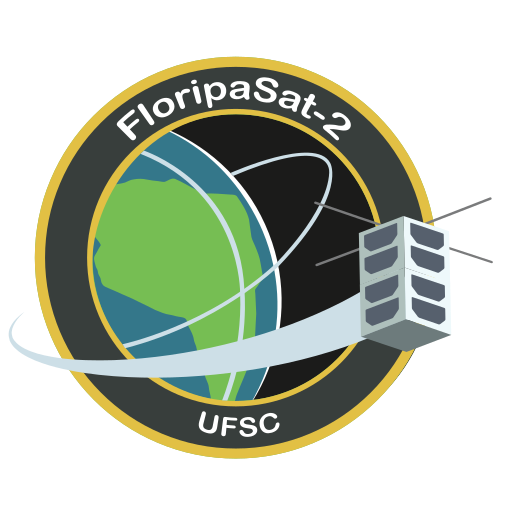
\includegraphics[width=0.5\textwidth]{figures/floripasat2-patch.png}
        \caption{FloripaSat-2 mission patch.}
        \label{fig:mission-patch}
    \end{center}
\end{figure}

    %
% requirements.tex
%
% Copyright (C) 2020 by SpaceLab.
%
% FloripaSat-2 Documentation
%
% This work is licensed under the Creative Commons Attribution-ShareAlike 4.0
% International License. To view a copy of this license,
% visit http://creativecommons.org/licenses/by-sa/4.0/.
%

%
% \brief Mission requirements chapter.
%
% \author Gabriel Mariano Marcelino <gabriel.mm8@gmail.com>
%
% \institution Universidade Federal de Santa Catarina (UFSC)
%
% \version 0.1.0
%
% \date 2020/06/06
%

\chapter{Mission Requirements} \label{ch:requirements}

\begin{enumerate}
    \item The power system shall be able to harvest solar energy.
    \item The power system shall be able to store energy for use when FloripaSat-2 is eclipsed.
    \item The power system shall supply energy to all other modules.
    \item The data handling system shall communicate with the other modules and store their data.
    \item The communications system shall send a beacon signal periodically using VHF radio.
    \item The communications system shall send the CubeSat telemetry using UHF radio.
    \item The communications system shall be able to receive telecommands and respond to them accordingly.
    \item The attitude system shall be able to perform a 1-axis stabilization of the CubeSat.
    \item FloripaSat-2 shall have the capability to receive and execute a shutdown telecommand, therefore ceasing all transmissions.
    \item The downlink transmissions shall be done once at a time, either telemetry or beacon.
    \item The ground station shall operate under the proper radio frequency communication licenses.
    \item FLoripaSat-2 shall comply with international and Brazilian radio license agreements and restrictions.
    \item The team shall build and operate a ground station for full communication with FloripaSat-2.
\end{enumerate}

    %
% schedule.tex
%
% Copyright (C) 2021 by SpaceLab.
%
% FloripaSat-2 Documentation
%
% This work is licensed under the Creative Commons Attribution-ShareAlike 4.0
% International License. To view a copy of this license,
% visit http://creativecommons.org/licenses/by-sa/4.0/.
%

%
% \brief Mission schedule chapter.
%
% \author Gabriel Mariano Marcelino <gabriel.mm8@gmail.com>
%
% \institution Universidade Federal de Santa Catarina (UFSC)
%
% \version 0.1.0
%
% \date 2020/06/06
%

\chapter{Mission Schedule} \label{ch:schedule}

\begin{table}[!h]
    \centering
    \begin{tabular}{cC{0.6cm}C{0.6cm}C{0.6cm}C{0.6cm}C{0.6cm}C{0.6cm}C{0.6cm}C{0.6cm}C{0.6cm}C{0.6cm}C{0.6cm}C{0.6cm}}
        \toprule[1.5pt]
        \multirow{3}{*}{\textbf{Activity}} & \multicolumn{12}{c}{\textbf{Month (2021)}} \\
                                           & Jan & Feb & Mar & Apr & May & Jun & Jul & Aug & Sep & Oct & Nov & Dez \\
        \midrule
        1                                  & \fc & \fc & \fc & \fc &     &     &     &     &     &     &     &     \\
        2                                  & \fc & \fc & \fc & \fc &     &     &     &     &     &     &     &     \\
        3                                  & \fc & \fc & \fc & \fc & \fc & \fc & \fc & \fc & \fc &     &     &     \\
        4                                  & \fc & \fc & \fc & \fc & \fc & \fc &     &     &     &     &     &     \\
        5                                  &     &     &     & \fc & \fc & \fc & \fc & \fc & \fc & \fc &     &     \\
        6                                  &     &     &     &     & \fc & \fc & \fc & \fc & \fc & \fc & \fc &     \\
        7                                  &     &     &     &     &     &     &     & \fc & \fc & \fc &     &     \\
        8                                  &     &     &     &     &     &     &     & \fc & \fc & \fc & \fc &     \\
        9                                  &     &     &     &     &     &     &     &     & \fc & \fc & \fc & \fc \\
        10                                 &     &     &     &     &     &     &     &     &     & \fc & \fc &     \\
        11                                 &     &     &     &     &     &     &     &     &     & \fc & \fc &     \\
        12                                 &     &     &     &     &     &     &     &     &     &     & \fc &     \\
        13                                 &     &     &     &     &     &     &     &     & \fc & \fc & \fc & \fc \\
        14                                 &     &     &     &     &     &     &     &     &     &     & \fc & \fc \\
        \bottomrule[1.5pt]
    \end{tabular}
    \caption{Mission schedule.}
    \label{tab:mission-schedule}
\end{table}

Each activity of \autoref{tab:mission-schedule} is decribed below:

\begin{enumerate}
    \item Acquisition and manufacturing of critical elements and components for the solo platform.
    \item Acquisition and manufacture of elements and components critical to the payload.
    \item Acquisition and manufacturing of critical elements and components for the solo segment.
    \item Compatibility tests between platform and payload in SpaceLab UFSC.
    \item Integration of the engineering model in SpaceLab UFSC.
    \item Preparation and suitability of the ground segment.
    \item Verification and validation of the engineering model at SpaceLab UFSC.
    \item Verification and validation of the flight model at SpaceLab UFSC.
    \item Data collection platforms installation.
    \item Verification and validation tests of Engineering Model compatibility with EMMN in the INPE / CRN in Natal.
    \item Environmental tests at the Integration and Testing Laboratory (LIT/INPE).
    \item Flight model acceptance and ground segment review.
    \item Ground segment delivery.
    \item Flight model delivery.
\end{enumerate}

    %
% overall.tex
%
% Copyright (C) 2021 by SpaceLab.
%
% FloripaSat-2 Documentation
%
% This work is licensed under the Creative Commons Attribution-ShareAlike 4.0
% International License. To view a copy of this license,
% visit http://creativecommons.org/licenses/by-sa/4.0/.
%

%
% \brief Overall description chapter.
%
% \author Gabriel Mariano Marcelino <gabriel.mm8@gmail.com>
%
% \institution Universidade Federal de Santa Catarina (UFSC)
%
% \version 0.1.0
%
% \date 2020/06/05
%

\chapter{Overall Description} \label{ch:overall}

.

\section{General Diagrams}

The CubeSat's subsystems are positioned in the 2U physical structure as exemplified in \autoref{fig:subsystems-positioning}. An exploded 3D view of the satellite is showed in \autoref{fig:exploded-view}.

\begin{figure}[!ht]
    \begin{center}
        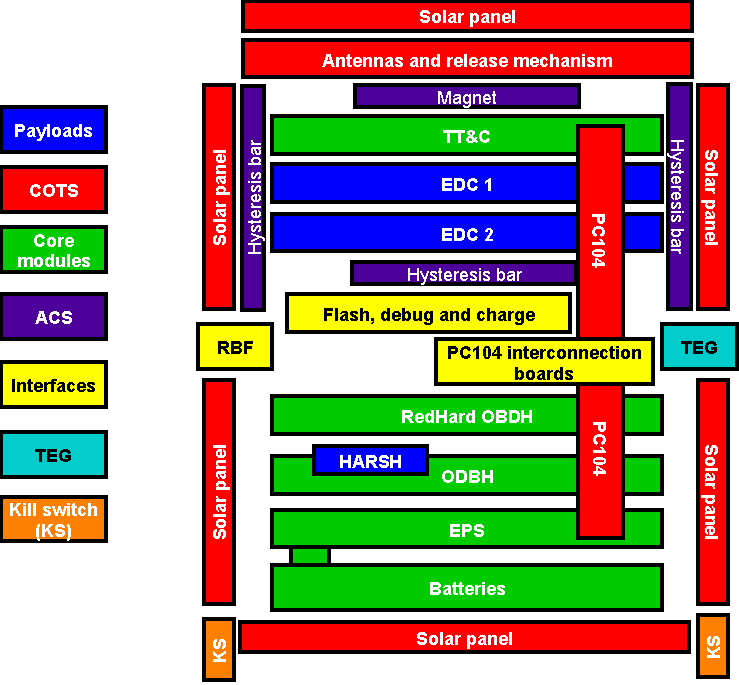
\includegraphics[width=0.7\textwidth]{figures/subsystems-positioning.pdf}
        \caption{Subsystems positioning.}
        \label{fig:subsystems-positioning}
    \end{center}
\end{figure}

\subsection{Power Diagram}

\begin{figure}[!ht]
    \begin{center}
        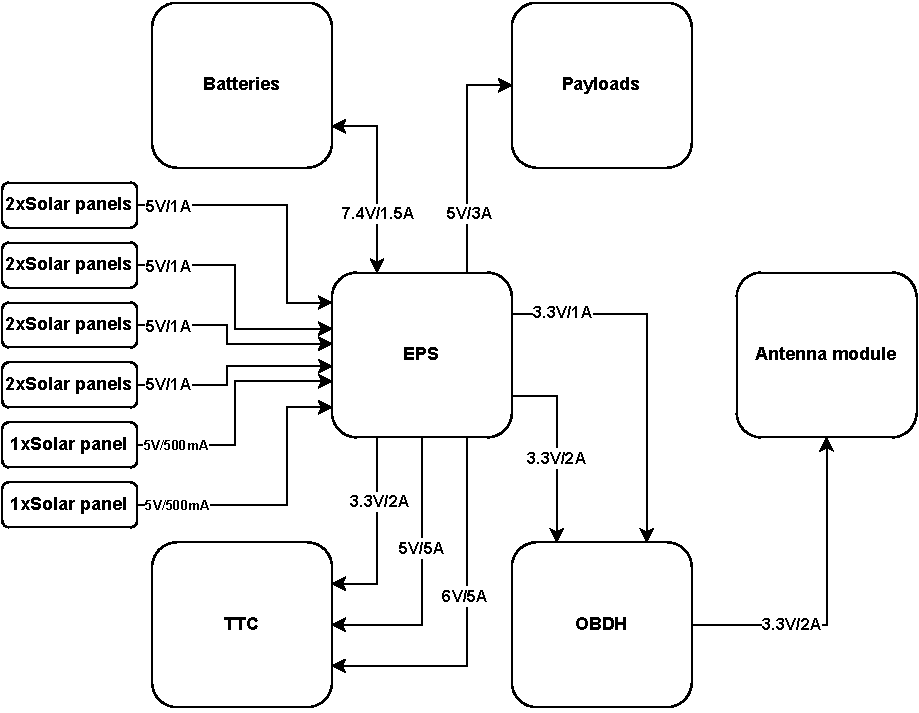
\includegraphics[width=\textwidth]{figures/power_diagram.pdf}
        \caption{Power diagram.}
        \label{fig:power-diagram}
    \end{center}
\end{figure}

%   TBD 
%   In \autoref{fig:datapath-diagram} there is a block diagram showing the satellite modules and the internal communication interfaces.

\subsection{Data Path Diagram}

\begin{figure}[!ht]
    \begin{center}
        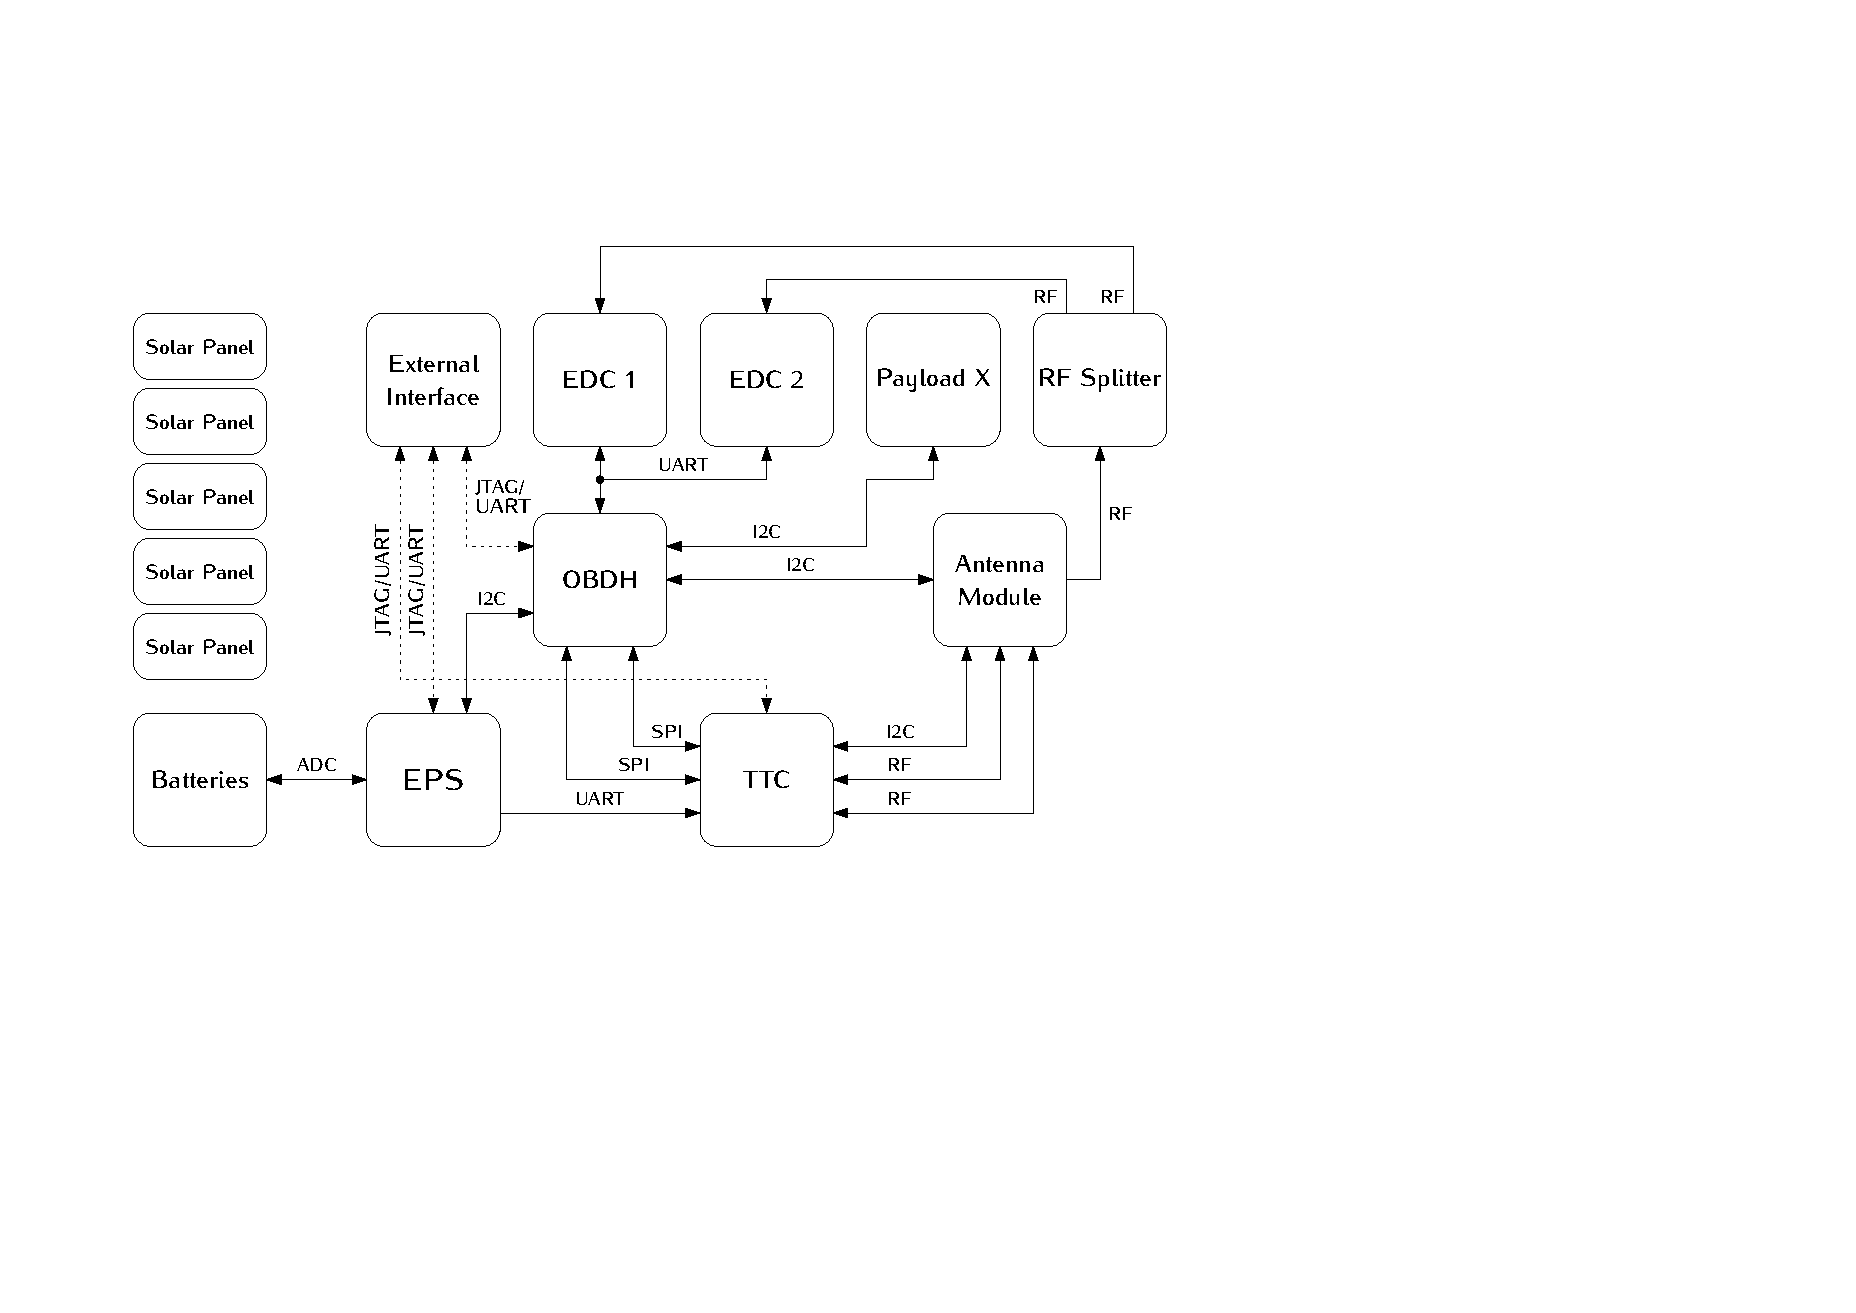
\includegraphics[width=\textwidth]{figures/data_path_diagram.pdf}
        \caption{Data path diagram.}
        \label{fig:data-path}
    \end{center}
\end{figure}

\subsection{Deployment Sequence}

The deployment sequence of the satellite is the routine to be executed just after the launch. The main objective of this operation is to the deploy the antennas and prepare the satellite to start its normal operation.

Just after the satellite is ejected from the deployer, the kill-switches enables the electric power and the three core modules execute the boot sequence (EPS, OBDH and TTC). The EPS module is ready to operate when the boot finishes. The OBDH and the TTC modules waits for a determined period before starting the normal execution.

As the OBDH and the TTC have access to the antenna module, both subsystem can control the deployment of the antennas. Following the CDS\nomenclature{\textbf{CDS}}{\textit{CubeSat Design Specification.}} specifications \cite{cds}, all CubeSats must wait 30 minutes to deploy the antennas and 45 minutes to transmit any RF signal. This way, the OBDH waits 45 minutes to send the deployment command to the antenna module. As redundancy, the TTC waits 55 minutes to execute the same operation.

The \autoref{fig:deployment-flowchart} has a flowchart that illustrates the deployment sequence of the service modules.

\begin{figure}[!ht]
    \begin{center}
        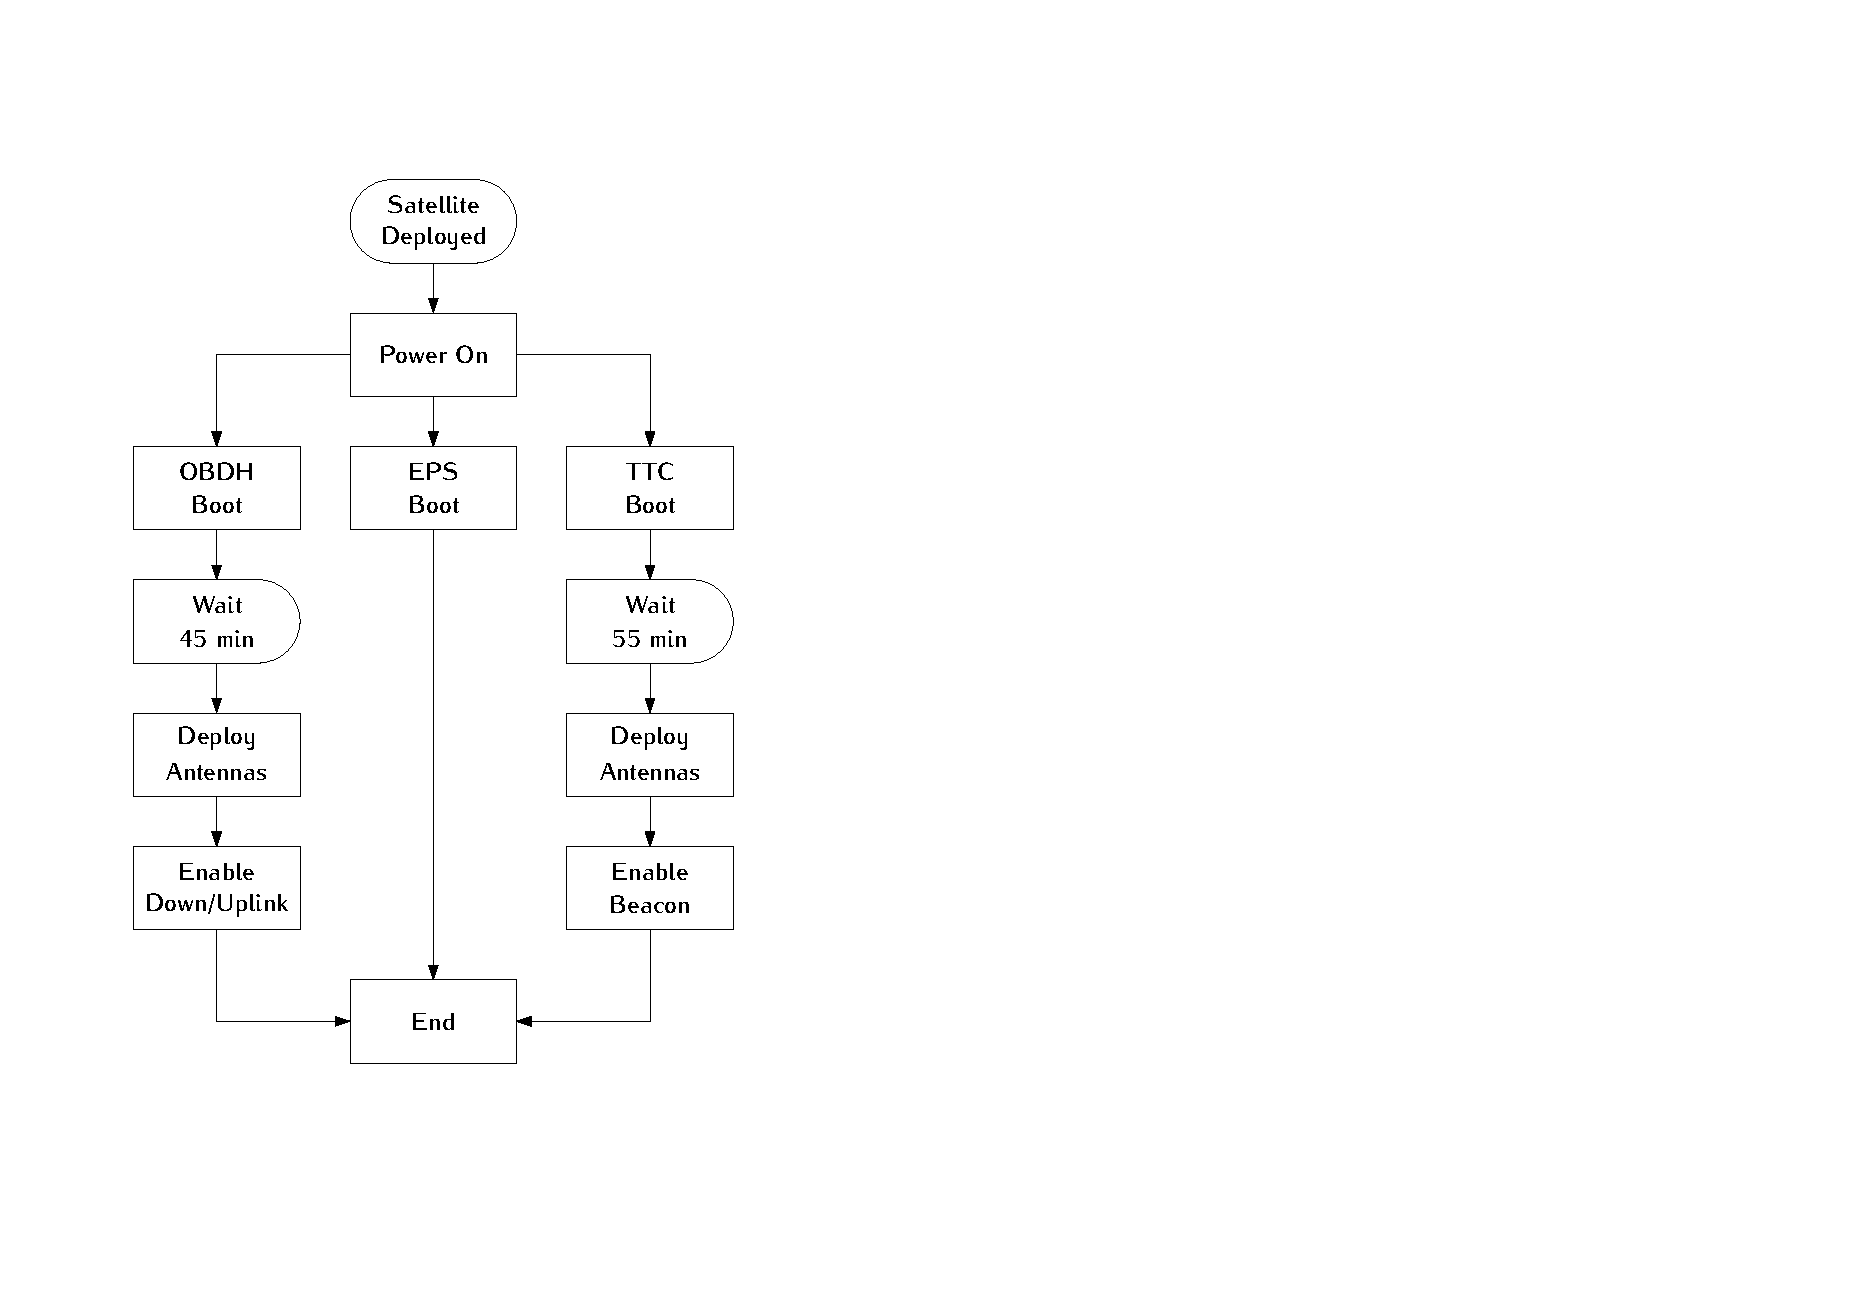
\includegraphics[width=0.5\textwidth]{figures/deployment-flowchart.pdf}
        \caption{Flowchart of the deployment sequence.}
        \label{fig:deployment-flowchart}
    \end{center}
\end{figure}

\subsection{Beacon Operation}

After the boot sequence of the beacon microcontroller, the operation of the beacon starts. The normal operation consist on reading the data from the EPS and the TTC modules, transmit the valid data (EPS or TTC package, in this order of priority), wait 60 seconds and repeat this sequence. The \autoref{fig:beacon-flowchart} has a flowchart of this behaviour.

\begin{figure}[!ht]
    \begin{center}
        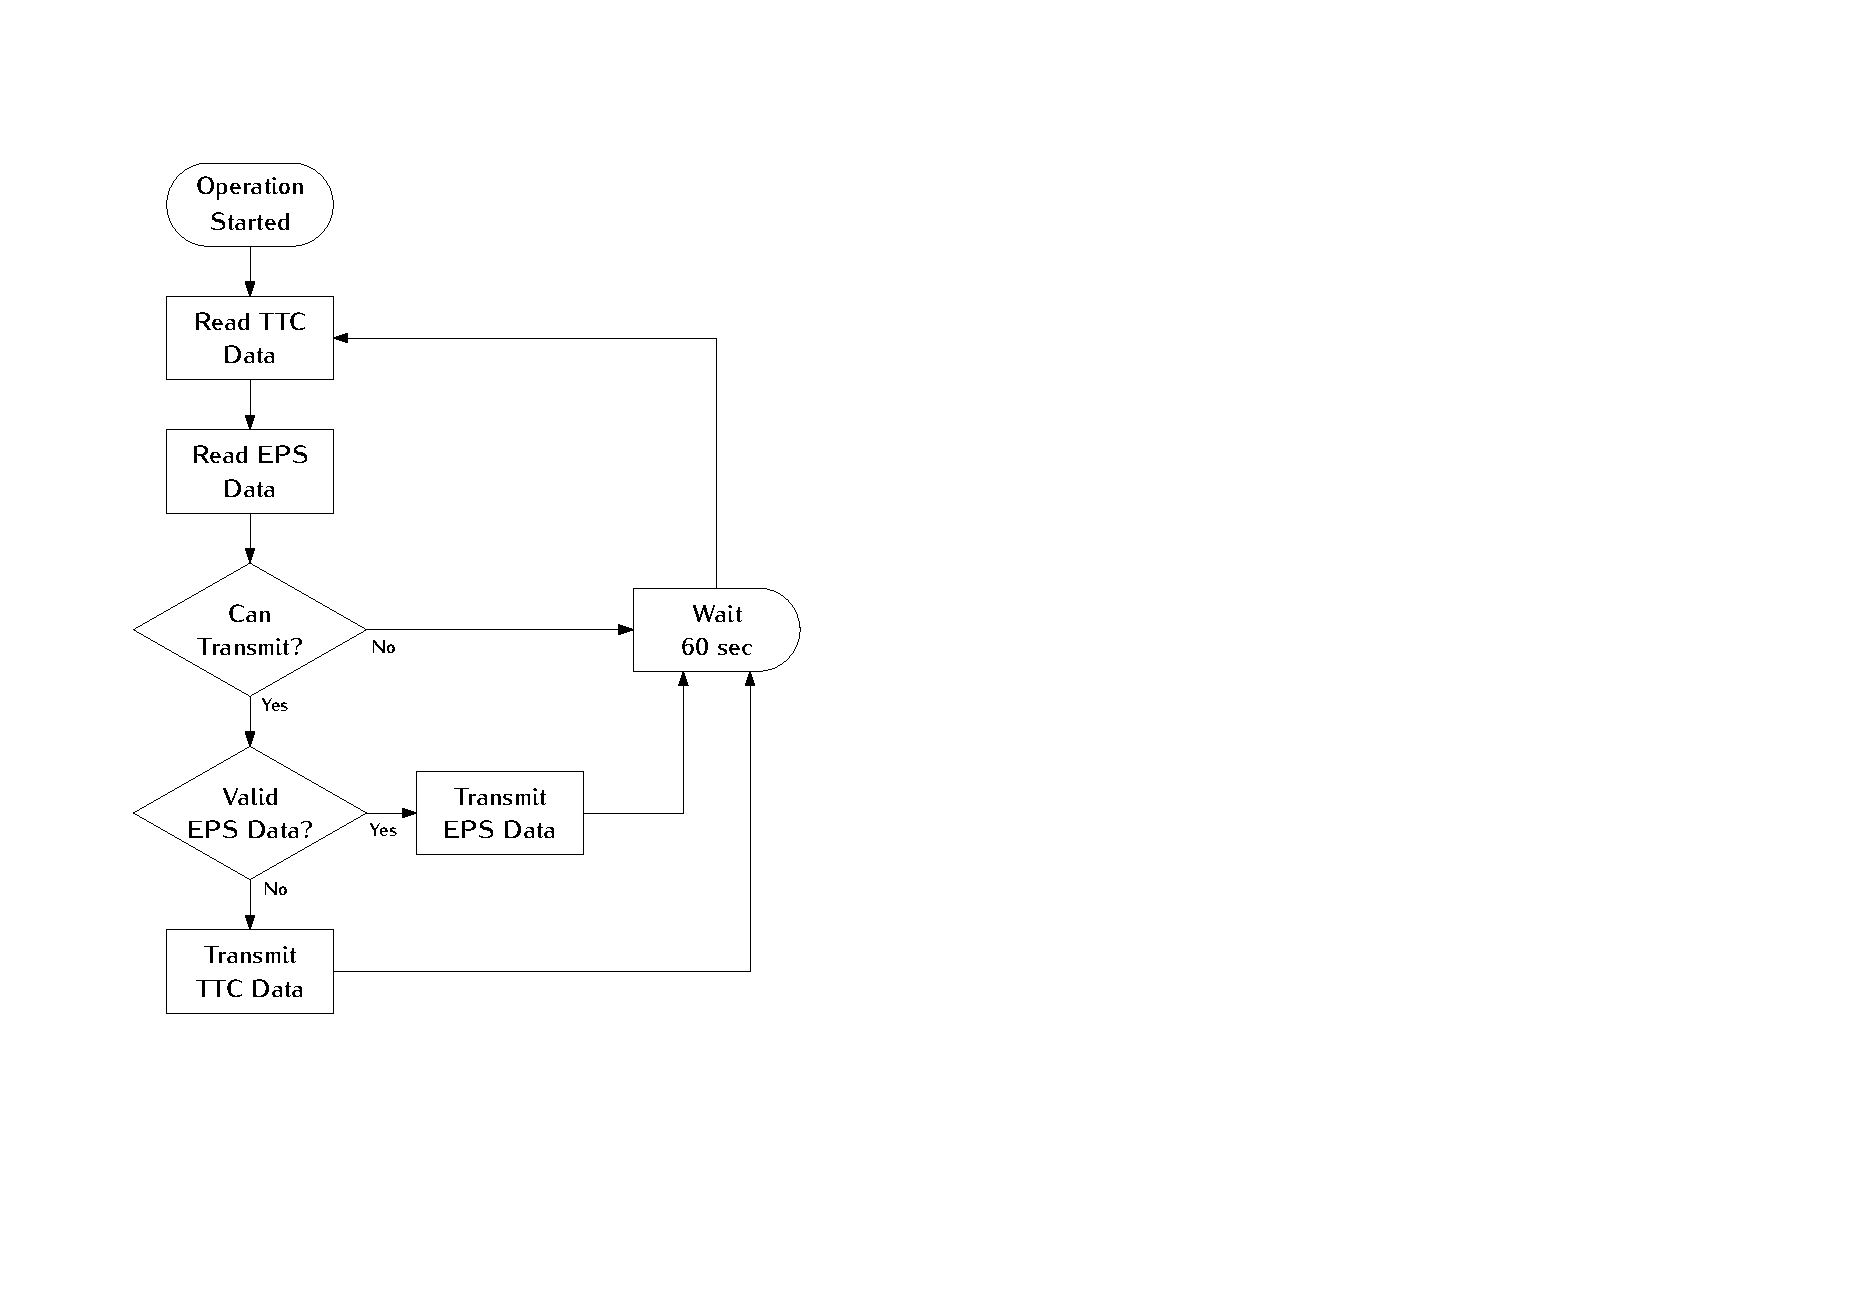
\includegraphics[width=0.55\textwidth]{figures/beacon-flowchart.pdf}
        \caption{Flowchart of the normal beacon operation.}
        \label{fig:beacon-flowchart}
    \end{center}
\end{figure}

\subsection{OBDH Operation}

After the boot sequence of the OBDH microcontroller, the operation of the OBDH starts. The normal operation consist on reading the housekeeping data from the EPS, TTC, payloads, antenna module and the OBDH (its own housekeeping data), save the read data on the non-volatile memory and transmit the housekeeping data of the satellite as a beacon. After that, it waits 60 seconds and check if a new telecommand was received, if true process the telecommand, if not, does nothing. After this sequence, these steps start again. The \autoref{fig:obdh-flowchart} has a flowchart of this behaviour.

\begin{figure}[!ht]
    \begin{center}
        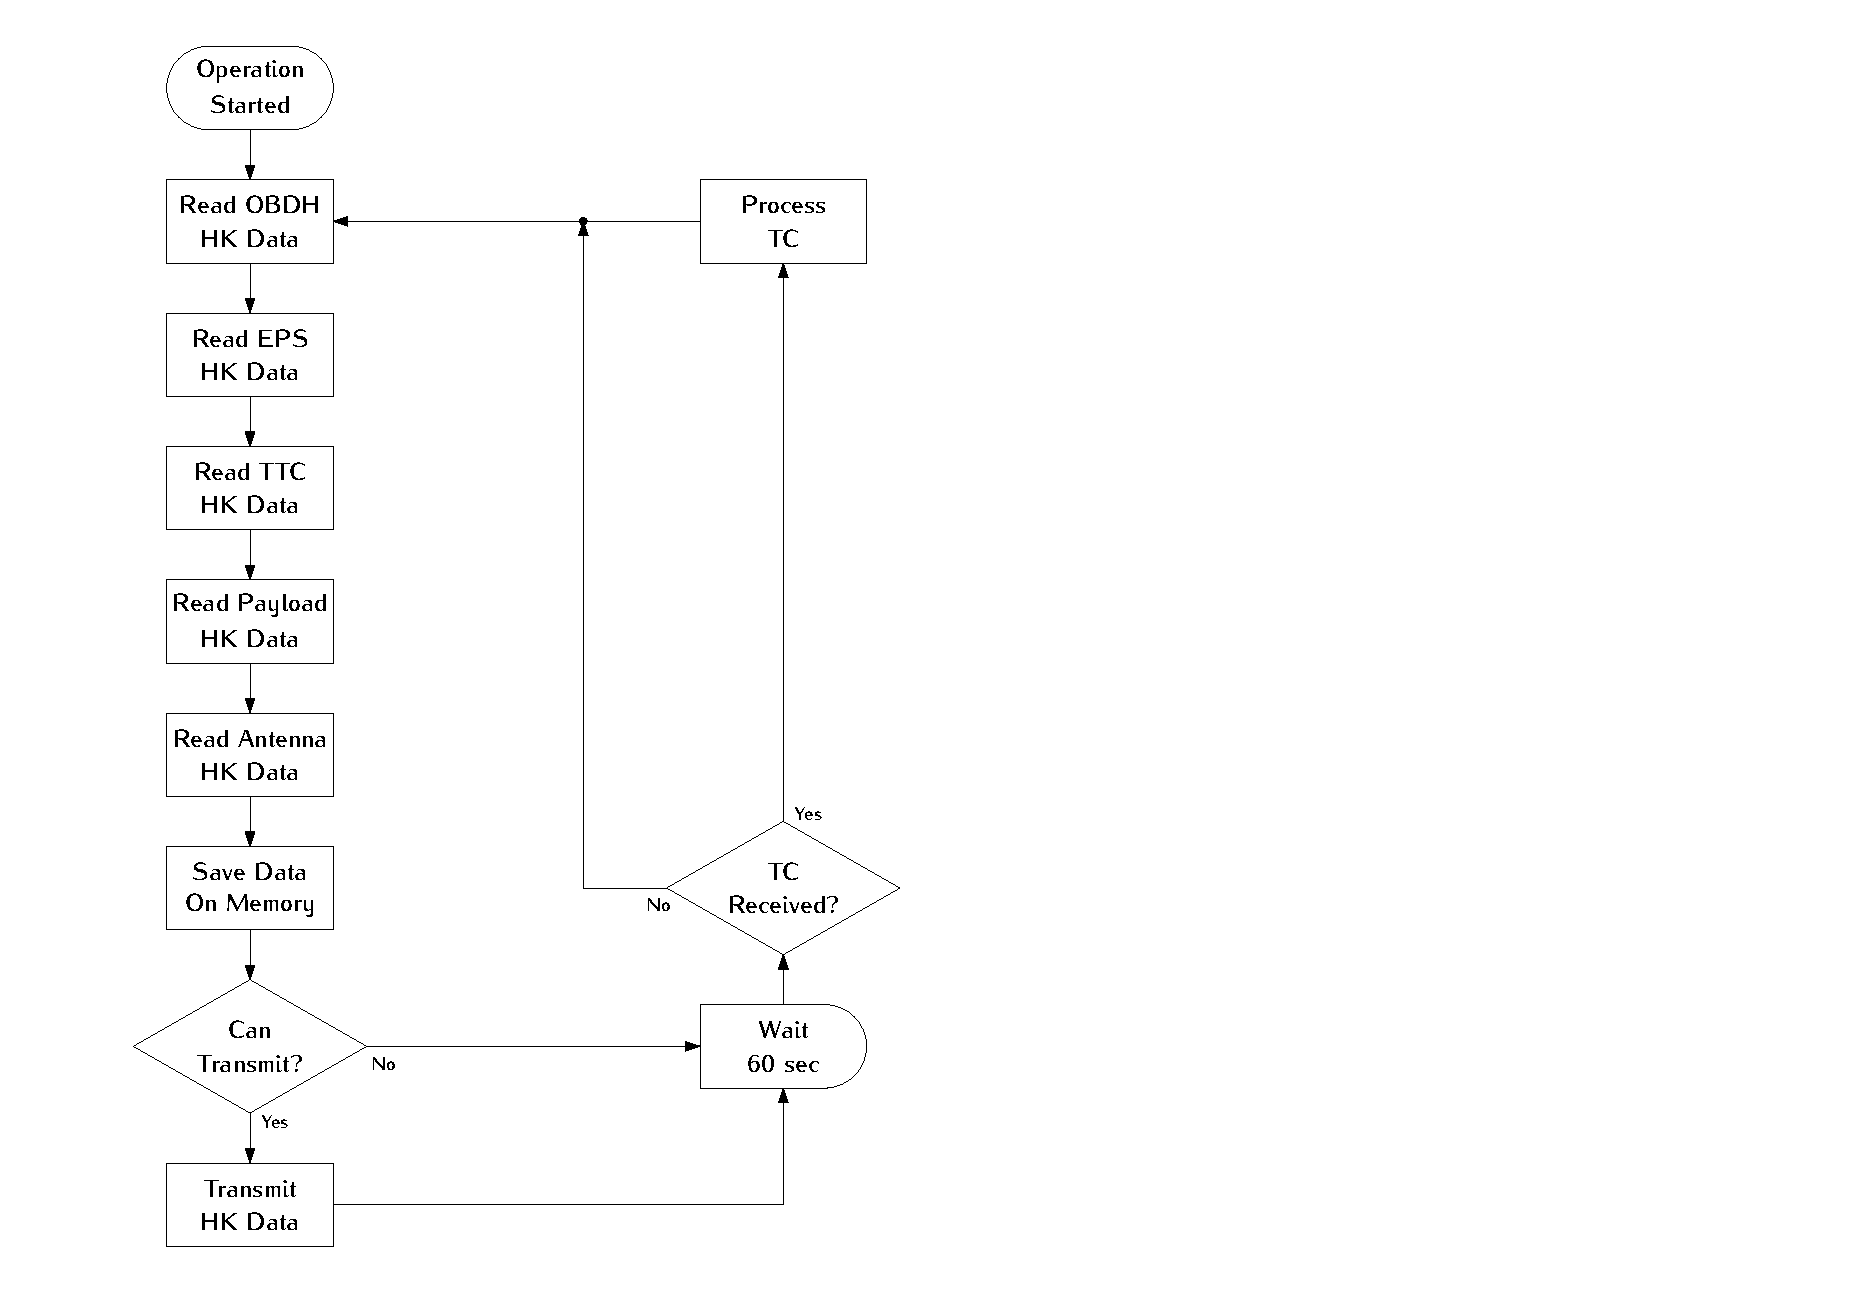
\includegraphics[width=0.63\textwidth]{figures/obdh-flowchart.pdf}
        \caption{Flowchart of the normal OBDH operation.}
        \label{fig:obdh-flowchart}
    \end{center}
\end{figure}

\subsubsection{Telecommand Processing}

.

\begin{figure}[!ht]
    \begin{center}
        \includegraphics[width=0.8\textwidth]{figures/tc-flowchart.pdf}
        \caption{Flowchart of telecommand processing.}
        \label{fig:tc-flowchart}
    \end{center}
\end{figure}

\subsection{EPS Operation}

The operation of the EPS microcontroller starts shortly after the release of the CubeSat in its orbit by the deployer.
In the first 60 minutes the module operation consist of reading the housekeeping data from its sensors and managing the duty cycles of the MPPT and heaters.
When operational, the TTC and OBDH modules send separete periodic requests to the EPS for fowarding the housekeeping data acquired.
The TTC receives a simplifed version while the OBDH receives a complete version of the data.
The \autoref{fig:eps-flowchart} has a flowchart of this behaviour.

\begin{figure}[!ht]
    \begin{center}
        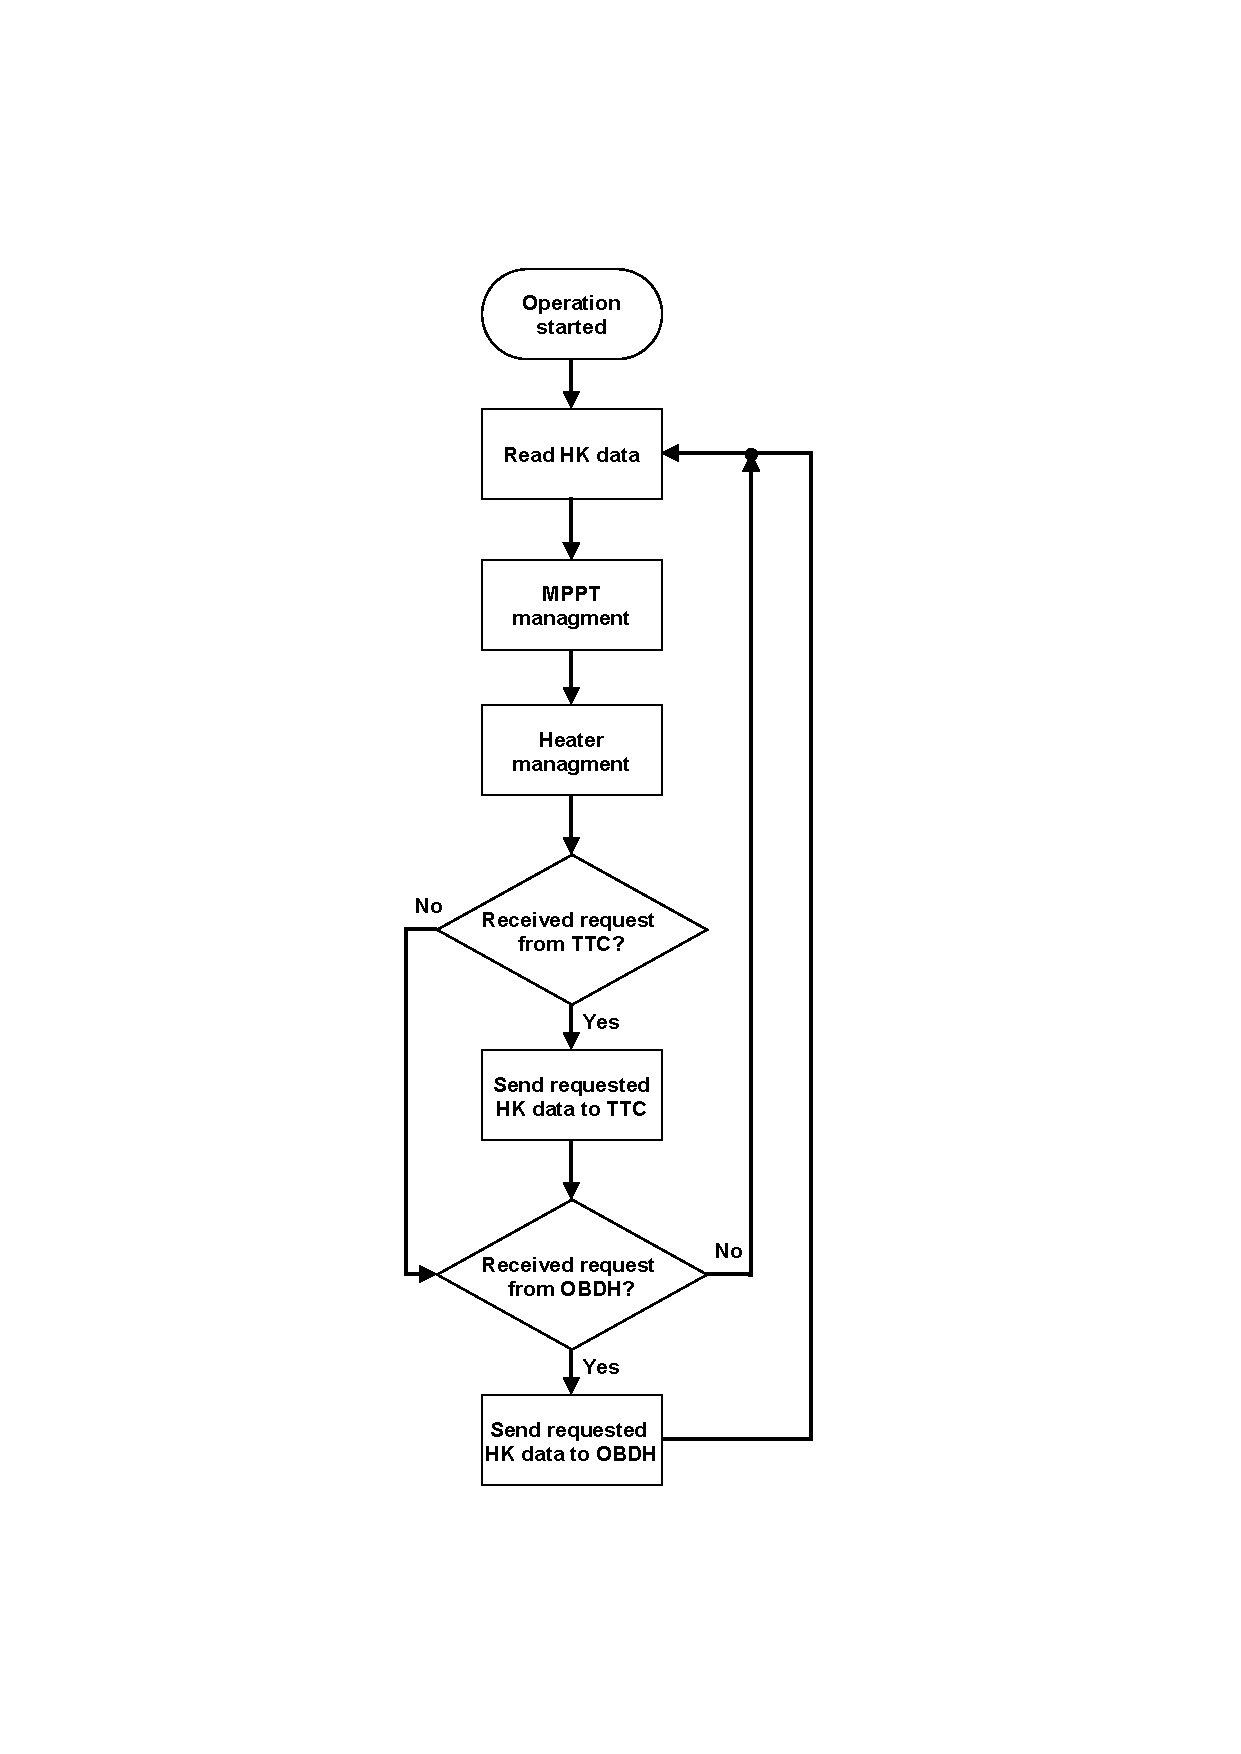
\includegraphics[width=0.88\textwidth]{figures/eps_flowchart.pdf}
        \caption{Flowchart of the normal EPS operation.}
        \label{fig:eps-flowchart}
    \end{center}
\end{figure}

\section{General Behaviour}

.

\section{Orbit Parameters and Analysis}

To define the orbit parameters and simulate the behaviour of the satellite during its operation, the GMAT\nomenclature{\textbf{GMAT}}{\textit{General Mission Analysis Tool.}} software was used \cite{gmat}. The orbit parameters was based on the FloripaSat-I TLE\nomenclature{\textbf{TLE}}{\textit{Two-Line Element.}}, but with a lower altitude. These parameters can be seen in \autoref{tab:orbit-parameters}.

\begin{table}[!h]
    \centering
    \begin{tabular}{lcc}
        \toprule[1.5pt]
        \textbf{Parameters} & \textbf{Value} & \textbf{Unit} \\
        \midrule
        Altitude                & 550           & km \\
        Eccentricity            & 0,0015051     & $^{\circ}$ \\
        Inclination             & 97,9750       & $^{\circ}$ \\
        RAAN                    & 85,5100       & $^{\circ}$ \\
        Arg. of Perigee (AOP)   & 194,87        & $^{\circ}$ \\
        TA                      & 99,8877       & $^{\circ}$ \\
        \bottomrule[1.5pt]
    \end{tabular}
    \caption{Initial orbit parameters (adapted from FloripaSat-I).}
    \label{tab:orbit-parameters}
\end{table}

The parameters of the simulation on GMAT was based on \cite{marino2016} and can be seen below:

\begin{itemize}
    \item Force model for gravitational field: ``\textit{Earth Gravitational Model 1996 (EGM96)}''
    \item Propagator: ``\textit{PrinceDorman78}''
    \item Drag coefficient: 2,2
    \item Drag atmosphere model: ``\textit{Mass Spectrometry and Incoherent Scatter (MSISE90)}''
    \item Epoch: 01 Jan 2022 11:59:28.000
\end{itemize}

The \autoref{fig:fsat2-gmat} shows the 3D representation of the FloripaSat-2 orbit simulation, \autoref{fig:fsat2-gmat-groundtrack} shows the ground track of the first day of operation.

\begin{figure}[!ht]
    \begin{center}
        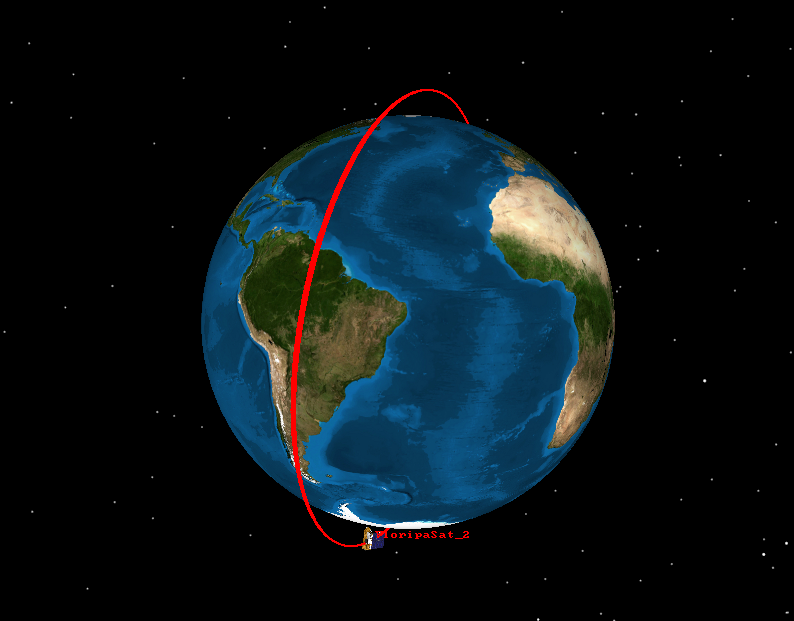
\includegraphics[width=0.6\textwidth]{figures/fsat2-gmat.png}
        \caption{FloripaSat-2 orbit simulation on GMAT.}
        \label{fig:fsat2-gmat}
    \end{center}
\end{figure}

\begin{figure}[!ht]
    \begin{center}
        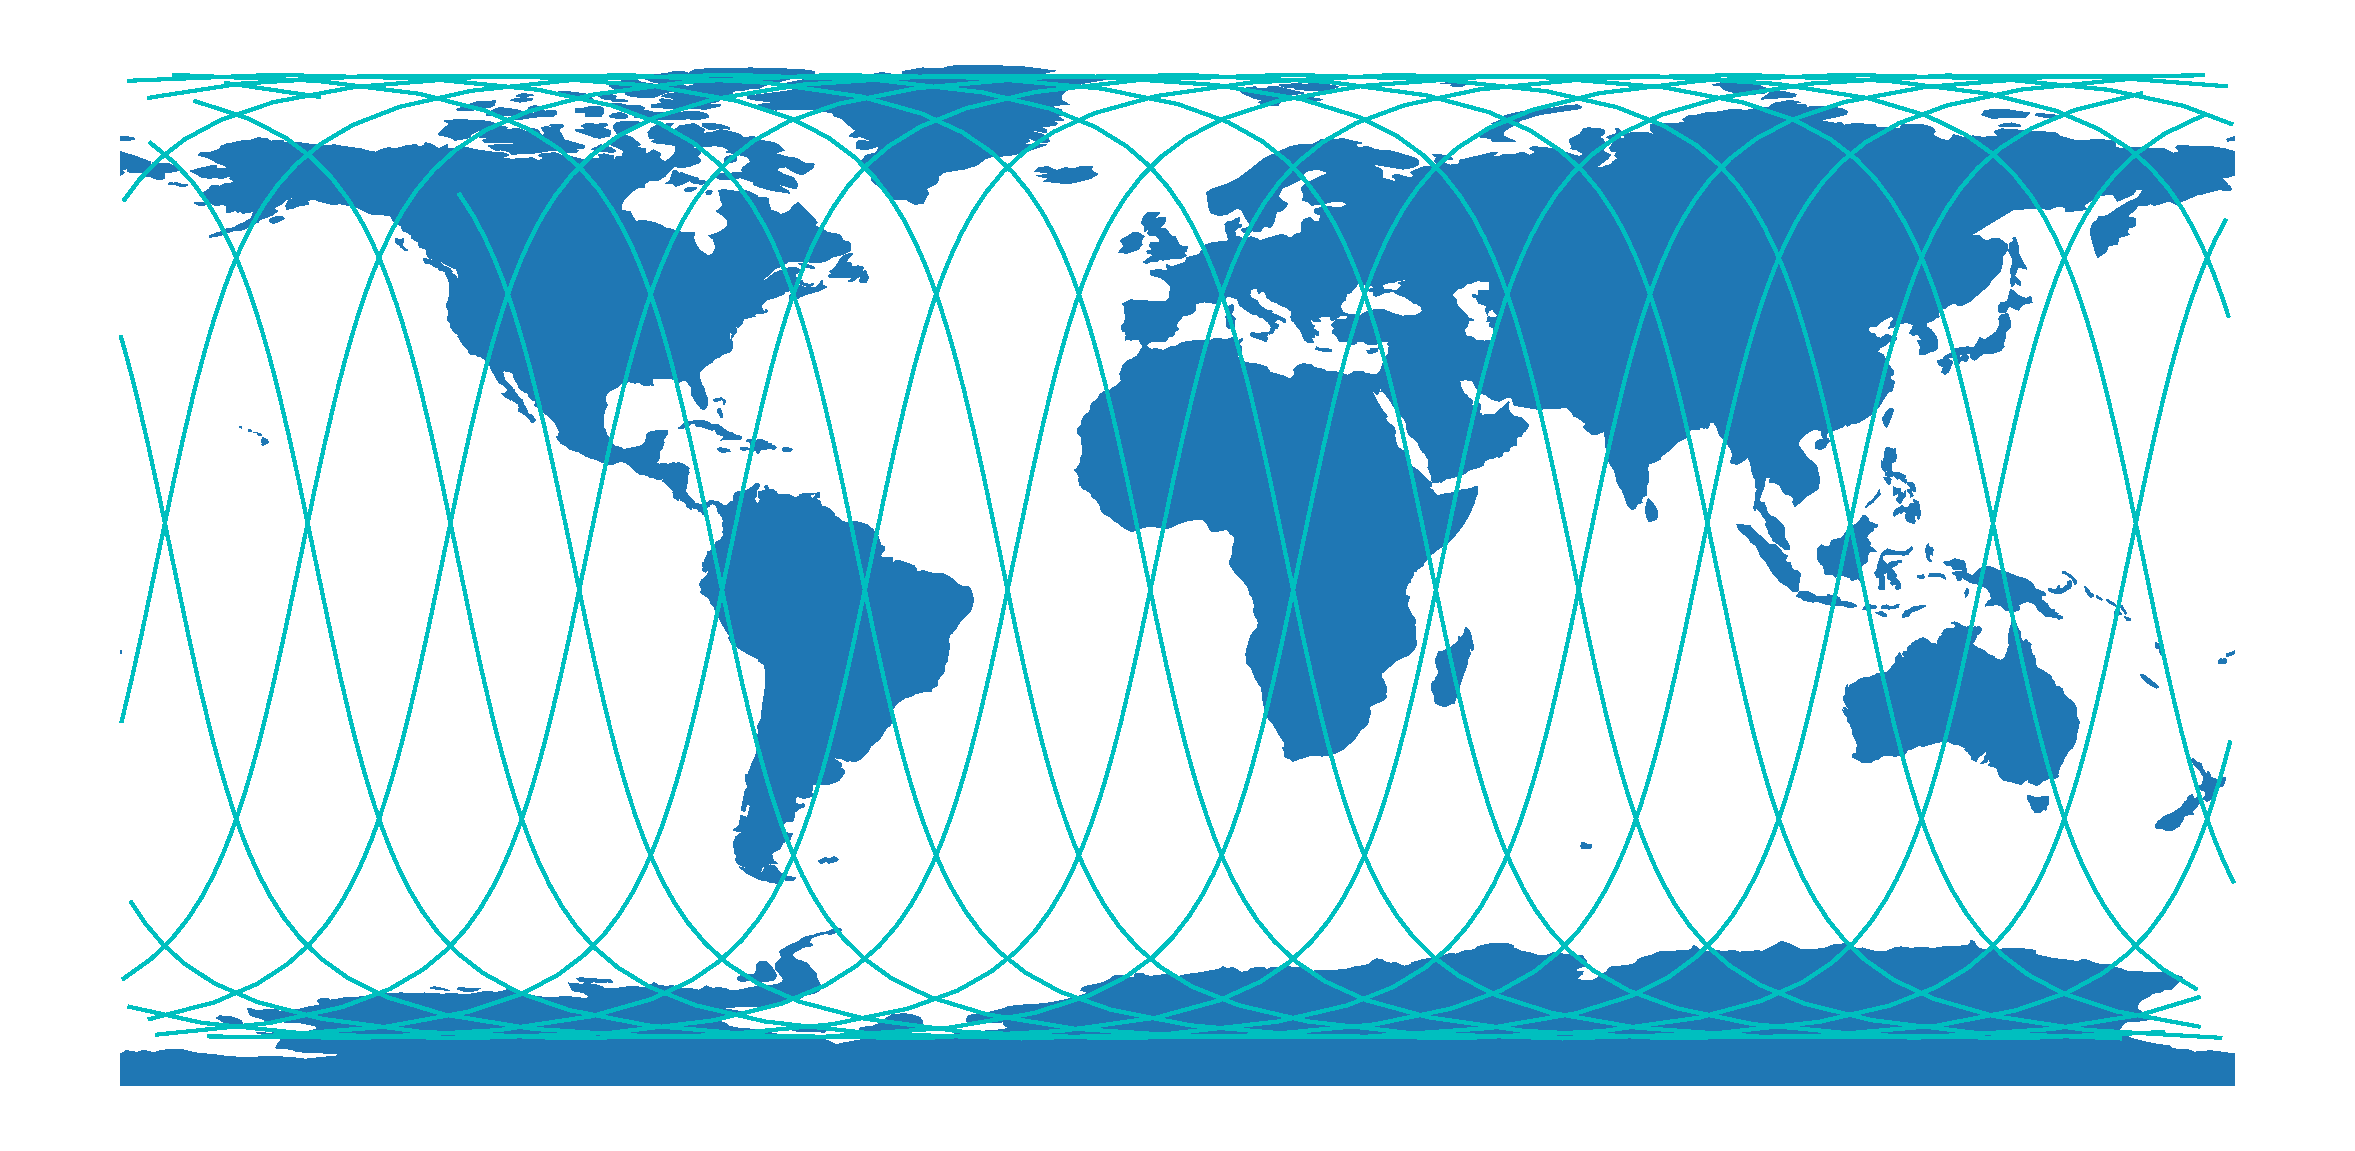
\includegraphics[width=\textwidth]{figures/fsat2-gmat-groundtrack.pdf}
        \caption{FloripaSat-2 simulated groundtrack.}
        \label{fig:fsat2-gmat-groundtrack}
    \end{center}
\end{figure}

The next sections present some analysis based on the results obtained on the simulations executed on GMAT.

The source files of the GMAT simulation are available in \cite{fsat2-mechanical}.

\subsection{Lifetime Analysis}

Considering the same parameters of FloripaSat-I, but with an initial altitude of 550 km, the simulations on GMAT showed that the satellite decays approximately in 2000 days ($\cong$ 5 years), as can be seen in \autoref{fig:lifetime-analysis}.

\begin{figure}[!ht]
    \begin{center}
        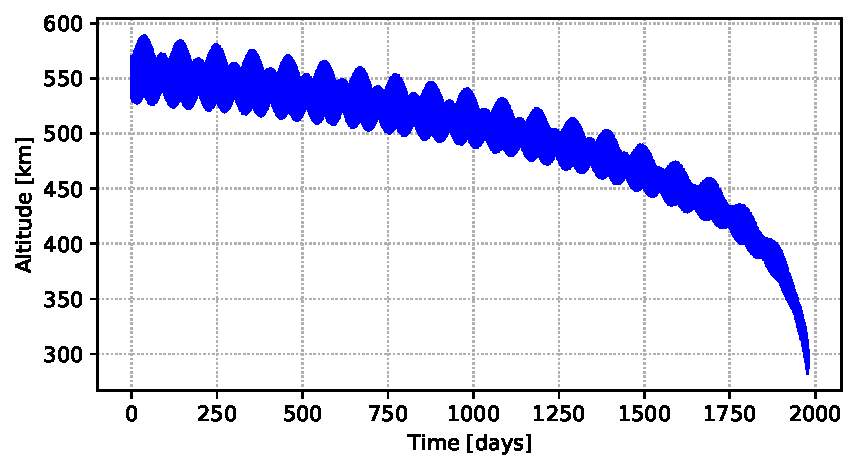
\includegraphics[width=\textwidth]{curves/lifetime.pdf}
        \caption{Lifetime analysis on GMAT.}
        \label{fig:lifetime-analysis}
    \end{center}
\end{figure}

\subsection{Ground Station Passes and Data Transfer Analysis}

Considering two ground stations, one at the SpaceLab installations in Florianópolis (27$^{\circ}$ 36' 00.9" S, 48$^{\circ}$ 31' 03.2" W) and other at the INPE/CRN installations in Natal (5$^{\circ}$ 50' 10.1" S, 35$^{\circ}$ 12' 27.5" W), both with a minimum elevation of 15$^{\circ}$, the following results were achieved during the simulations on GMAT (\autoref{tab:grs-contacts-analysis}).

\begin{table}[!h]
    \centering
    \begin{tabular}{lccc}
        \toprule[1.5pt]
        \textbf{Parameter} & \textbf{UFSC Station} & \textbf{INPE-RN Station} & \textbf{Unit} \\
        \midrule
        Minimum elevation to a valid contact    & 15    & 15    & $^{\circ}$ \\
        Number of contacts                      & 143   & 125   & - \\
        Minimum contact period                  & 24    & 34    & sec \\
        Maximum contact period                  & 395   & 394   & sec \\
        Average contact period                  & 303   & 298   & sec \\
        Total contact period                    & 43394 & 37205 & sec \\
        \bottomrule[1.5pt]
    \end{tabular}
    \caption{Ground station contacts analysis during the first 60 days of operation.}
    \label{tab:grs-contacts-analysis}
\end{table}

As can be seen from \autoref{tab:grs-contacts-analysis}, during the first 60 days of operation, considering the two main ground stations that will contact the satellite, the total contact period is 80599 seconds (43394 + 37205). With the data rate of the downlink/uplink as 4800 bps, this time period will allow a data transfer of 48359400 bytes (or 46,12 M$_{i}$B) between FloripaSat-2 and the Earth. Using the lifetime of the satellite from the previous analysis (2000 days), and an average data transfer per day of 805990 bits, the total theoretical raw data transfer during the whole operation of the satellite will be approximately 1,5 G$_{i}$B.

These values can be even bigger if a smaller minimum elevation is considered, or with more ground stations in other locations.

\section{Power Budget}

According to section 10.3 of \cite{larson2005}, the power budget of satellite can be determined through three steps:

\begin{enumerate}
    \item Prepare operating power budget
    \item Size the battery
    \item Estimate power degradation over mission life
\end{enumerate}

\subsection{Operating Power Budget}

\begin{table}[!h]
    \centering
    \begin{tabular}{lccccc}
        \toprule[1.5pt]
        \multirow{2}{*}{\textbf{Module}} & \multirow{2}{*}{\textbf{Voltage [V]}}    & \multicolumn{2}{c}{\textbf{Current [mA]}} & \multicolumn{2}{c}{\textbf{Power [mW]}} \\
                                         &                                          & \textbf{Min.} & \textbf{Max.}             & \textbf{Min.} & \textbf{Max.} \\
        \midrule
        OBDH                & 3,3   & TBD   & TBD   & TBD   & TBD \\
        TTC ($\mu$C)        & 3,3   & TBD   & TBD   & TBD   & TBD \\
        TTC (radio module)  & 5     & TBD   & 650   & TBD   & 3250 \\
        EPS (digital part)  & 3,3   & TBD   & TBD   & TBD   & TBD \\
        EPS (heater)        & 3,3   & TBD   & TBD   & TBD   & TBD \\
        Antenna module      & 3,3   & TBD   & TBD   & TBD   & TBD \\
        Payload EDC         & 5     & 250   & 250   & 1250  & 1250 \\
        Payload-X           & 5     & TBD   & TBD   & TBD   & TBD \\
        Payload Harsh       & 3,3   & TBD   & TBD   & TBD   & TBD \\
        \bottomrule[1.5pt]
    \end{tabular}
    \caption{Power requirements of the subsystems and payloads of the satellite.}
    \label{tab:power-requirements}
\end{table}

Assumptions:

\begin{itemize}
    \item One of the EDC payload is always off (cold redundancy).
    \item The Payload-X and the Harsh payload are turned on just during limited periods.
\end{itemize}

\subsection{Battery Sizing}

.

\subsection{Power Degradation Over Mission Life}

\begin{itemize}
    \item Solar panels degradation
    \item Battery degradation
\end{itemize}

\section{Link Budget}

The link budget of all radio links of the satellite is available in \autoref{tab:link-budget-results}.

\begin{table}[!h]
    \centering
    \begin{tabular}{L{0.3\textwidth}ccccc}
        \toprule[1.5pt]
        \textbf{Variable} & \textbf{Beacon} & \textbf{Downlink} & \textbf{Uplink} & \textbf{Uplink (Payload)} & \textbf{Unit}\\
        \midrule
        Frequency                       & 145,97    & 436,9     & 436,9     & 401,635   & MHz \\
        Modulation                      & GMSK      & GMSK      & GMSK      & BPSK      & - \\
        Protocol                        & NGHam     & NGHam     & NGHam     & SBCD      & - \\
        Transmit power                  & 30        & 30        & 47        & ??        & dBm \\
        FSPL                            & 144,8     & 154,3     & 154,3     & ??        & dB \\
        Other losses                    & 5         & 5         & 7         & 5         & dB \\
        Receive antenna gain            & 12        & 15.5      & 0         & 0         & dBi \\
        Receiver noise temp.            &           &           &           &           & K \\
        Antenna noise temp.             &           &           &           &           & K \\
        System noise temp.              &           &           &           &           & K \\
        Data rate                       & 1200      & 4800      & 4800      & 400       & bps \\
        Received SNR                    & 30,87     & 17,35     & 31,60     & ??        & dB \\
        SNR required for $10^{-5}$ BER*  & 9,6       & 9,6       & 9,6       & 9,6       & dB \\
        Link margin                     & $\leq$ 21,27 & $\leq$ 7,75 & $\leq$ 22 & $\leq$ ?? & dB \\
        \bottomrule[1.5pt]
    \end{tabular}
    \caption{Link budget results.}
    \label{tab:link-budget-results}
\end{table}

All equations and steps used to obtain the results of \autoref{tab:link-budget-results} are available in \autoref{anx:link-budget}.

\section{PC-104 Bus}

\subsection{Interface}

To electrically connect all the satellite modules, a PC-104 bus standard is being used. This bus is composed by 104 lines disposed by four rows of 26 pins each (with a vertical and horizontal pitch of 2,54 mm).

Using the \autoref{fig:pc104-ref-diagram} as reference, all used positions and signals of the PC-104 bus are presented in \autoref{tab:pc104-pinout}. The \autoref{tab:pc104-signals} describes each signal and which modules are connected to them.

\begin{figure}[!ht]
    \begin{center}
        \includegraphics[width=0.5\textwidth]{figures/pc104-diagram}
        \caption{Reference diagram of the PC-104 bus (top view of a generic module).}
        \label{fig:pc104-ref-diagram}
    \end{center}
\end{figure}

\begin{table}[!h]
    \centering
    \begin{tabular}{cllll}
        \toprule[1.5pt]
        \textbf{Pin Row}   & \textbf{H1 Odd}  & \textbf{H1 Even} & \textbf{H2 Odd} & \textbf{H2 Even} \\
        \midrule
        1-2                & -                & -                & -               & -                \\
        3-4                & -                & -                & EDC\_1\_EN      & EDC\_2\_EN       \\
        5-6                & -                & -                & BE\_UART\_RX    & -                \\
        7-8                & RA\_GPIO\_0      & RA\_GPIO\_1      & BE\_UART\_TX    & GPIO\_0          \\
        9-10               & RA\_GPIO\_2      & BE\_EN           & -               & -                \\
        11-12              & RA\_RESET        & RA\_EN           & BE\_SPI\_MOSI   & BE\_SPI\_CLK     \\
        13-14              & -                & -                & BE\_SPI\_CS     & BE\_SPI\_MISO    \\
        15-16              & -                & -                & -               & -                \\
        17-18              & EDC\_UART\_RX/TX & PLX\_EN          & -               & GPIO\_1          \\
        19-20              & EDC\_UART\_TX/RX & GPIO\_2          & -               & GPIO\_3          \\
        21-22              & -                & -                & -               & GPIO\_4          \\
        23-24              & -                & -                & -               & -                \\
        25-26              & -                & -                & PL\_VCC         & PL\_VCC          \\
        27-28              & -                & -                & TTC\_VCC        & TTC\_VCC         \\
        29-30              & GND              & GND              & GND             & GND              \\
        31-32              & GND              & GND              & GND             & GND              \\
        33-34              & -                & -                & -               & -                \\
        35-36              & RA\_SPI\_CLK     & -                & ANT\_VCC        & ANT\_VCC         \\
        37-38              & RA\_SPI\_MISO    & -                & -               & -                \\
        39-40              & RA\_SPI\_MOSI    & RA\_SPI\_CS      & -               & -                \\
        41-42              & PL\_I2C\_SDA     & -                & -               & GPIO\_5          \\
        43-44              & PL\_I2C\_SCL     & -                & -               & -                \\
        45-46              & OBDH\_VCC        & OBDH\_VCC        & BAT\_VCC        & BAT\_VCC         \\
        47-48              & PL\_VCC          & PL\_VCC          & -               & -                \\
        49-50              & RA\_VCC          & RA\_VCC          & EPS\_I2C\_SDA   & -                \\
        51-52              & BE\_VCC          & BE\_VCC          & EPS\_I2C\_SCL   & -                \\
        \bottomrule[1.5pt]
    \end{tabular}
    \caption{PC-104 bus pinout.}
    \label{tab:pc104-pinout}
\end{table}

\begin{table}[!h]
    \centering
    \begin{tabular}{lL{0.18\textwidth}L{0.17\textwidth}L{0.33\textwidth}}
        \toprule[1.5pt]
        \textbf{Signal}  & \textbf{Pin(s)} & \textbf{Used By}     & \textbf{Description} \\
        \midrule
        GND              & H1-29/30/31/32, H2-29/30/31/32 & All   & Ground reference \\
        BAT\_VCC         & H2-45, H2-46    & EPS                  & Battery terminals (+) \\
        ANT\_VCC         & H2-35, H2-36    & EPS, ANT             & Antenna power supply (3.3 V) \\
        OBDH\_VCC        & H1-45, H1-46    & EPS, OBDH            & OBDH power supply (3.3 V) \\
        TTC\_VCC         & H2-27, H2-28    & EPS, TTC             & TTC power supply (3.3 V) \\
        PL\_VCC          & H1-47/48, H2-25/26 & EPS, EDC 1/2, Payload X & Payloads power supply (5 V) \\
        RA\_VCC          & H1-49, H1-50    & EPS, TTC             & Main radio power supply (5 V) \\
        BE\_VCC          & H1-51, H1-52    & EPS, TTC             & Beacon power supply (6 V) \\
        RA\_SPI\_CLK     & H1-35           & OBDH, TTC            & CLK signal of the main radio SPI bus \\
        RA\_SPI\_MISO    & H1-37           & OBDH, TTC            & MISO signal of the main radio SPI bus \\
        RA\_SPI\_MOSI    & H1-39           & OBDH, TTC            & MOS signal of the main radio SPI bus \\
        RA\_SPI\_CS      & H1-40           & OBDH, TTC            & CS signal of the main radio SPI bus \\
        EPS\_I2C\_SDA    & H2-49           & OBDH, EPS            & SDA signal of the EPS I2C bus \\
        EPS\_I2C\_SCL    & H2-51           & OBDH, EPS            & SCL signal of the EPS I2C bus \\
        BE\_UART\_RX     & H2-5            & EPS, TTC             & EPS TX, Beacon RX (UART bus) \\
        BE\_UART\_TX     & H2-7            & EPS, TTC             & EPS RX, Beacon TX (UART bus) \\
        EDC\_UART\_TX/RX & H1-25           & OBDH, EDC 1/2        & OBDH TX, EDCs RX (UART bus) \\
        EDC\_UART\_RX/TX & H1-27           & OBDH, EDC 1/2        & OBDH RX, EDCs TX (UART bus) \\
        BE\_EN           & H1-10           & EPS, TTC             & Beacon radio power enable \\
        RA\_EN           & H1-12           & EPS, OBDH            & Main radio power enable \\
        EDC\_1\_EN       & H2-3            & OBDH, EDC 1          & EDC 1 enable signal \\
        EDC\_2\_EN       & H2-4            & OBDH, EDC 2          & EDC 2 enable signal \\
        PLX\_EN          & H1-18           & OBDH, Payload X      & Payload X enable (GPIO) \\
        PL\_I2C\_SDA     & H1-41           & OBDH, Payload X      & SDA signal of the payload I2C bus \\
        PL\_I2C\_SCL     & H1-43           & OBDH, Payload X      & SCL signal of the payload I2C bus \\
        GPIO\_N          & H1-20, H2-8/18/20/22/42  & OBDH        & GPIO pin (not used) \\
        \bottomrule[1.5pt]
    \end{tabular}
    \caption{PC-104 bus signal description.}
    \label{tab:pc104-signals}
\end{table}

The distribution pattern of pins adopted in this project is a mix of multiple different patterns from CubeSat modules manufacturers, like GomSpace, ISIS and Endurosat. Some pins are positioned to attend specific project requirements, and it is possible that the adopted pattern is not totally compatible to some commercial modules.

Beyond the PC-104 bus, there are some signals connected directly by wires and cables, like the control and power pins of the antenna module, the battery charger and the programming ports.

\subsection{Form Factor}

The form factor follows a similar specification of the PC-104 standard\cite{pc104-specification}.
The connector used for the interface differs given the module, the isolation heigth and presence of pin or receptable are definied from the overall stack up of the subystems inside the CubeSat 2U structure.
% TBD: include reference to mechanical design here
The core modules have smoothed edges and some linear mounting hole distances different from the standard, these are according to fit in a CubeSat form factor.
The PC-104 form factor used can be seen in \autoref{fig:pc104-form-factor}.

\begin{figure}[!ht]
    \begin{center}
        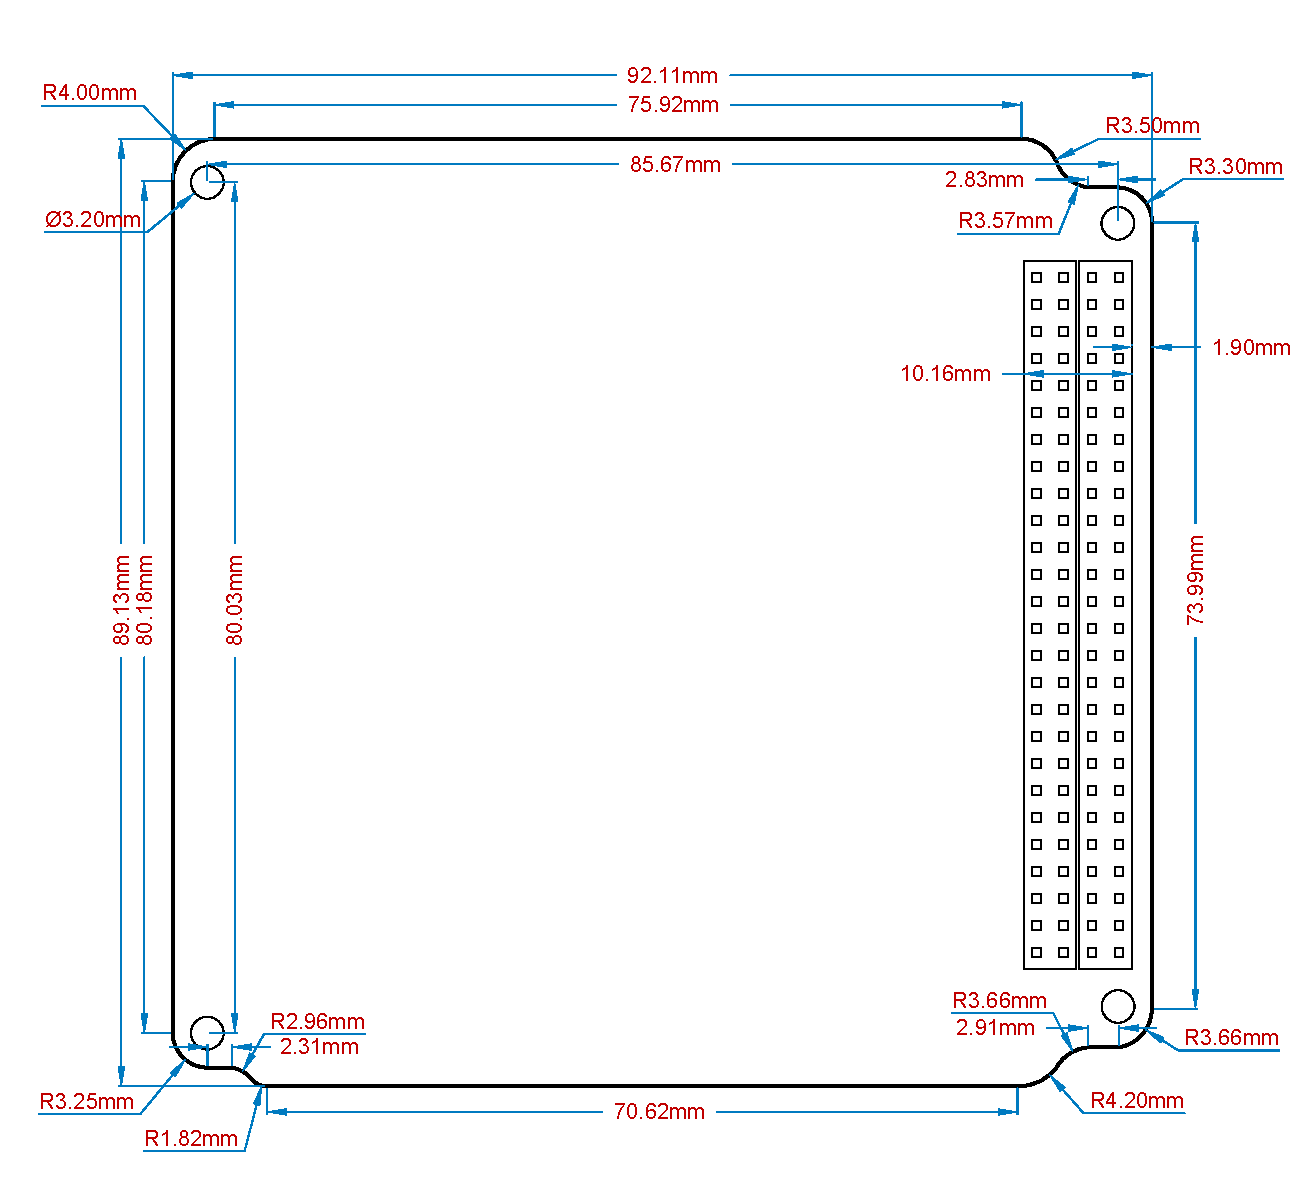
\includegraphics[width=0.75\textwidth]{figures/pc104-form-factor.pdf}
        \caption{PC-104 Form Factor.}
        \label{fig:pc104-form-factor}
    \end{center}
\end{figure}

\section{Telecommunication}

This section describes the configuration and behaviour of the telecommunication subsystems of the satellite. There are three types links available in the CubeSat: beacon, downlink and uplink. The beacon link is a periodic transmission of packets with a basic telemetry data of the satellite (containing data from the EPS or TTC subsystems). The downlink is the link used to receive all data from the satellite, including the results of all experiments, telemetry data and telecommands feedback. And the uplink is used for send telecommands from a ground station to the satellite.

The payload of all packets follows the same structure, with an ID number, the source address (callsign) and the content of the packet (variable according to each type of packet). Following the NGHam protocol characteristics, the maximum length of a packet, including the ID and the source address, is 220 bytes. The \autoref{fig:fsat-pkt-structure} illustrates this packet structure.

\begin{figure}[!ht]
    \begin{center}
        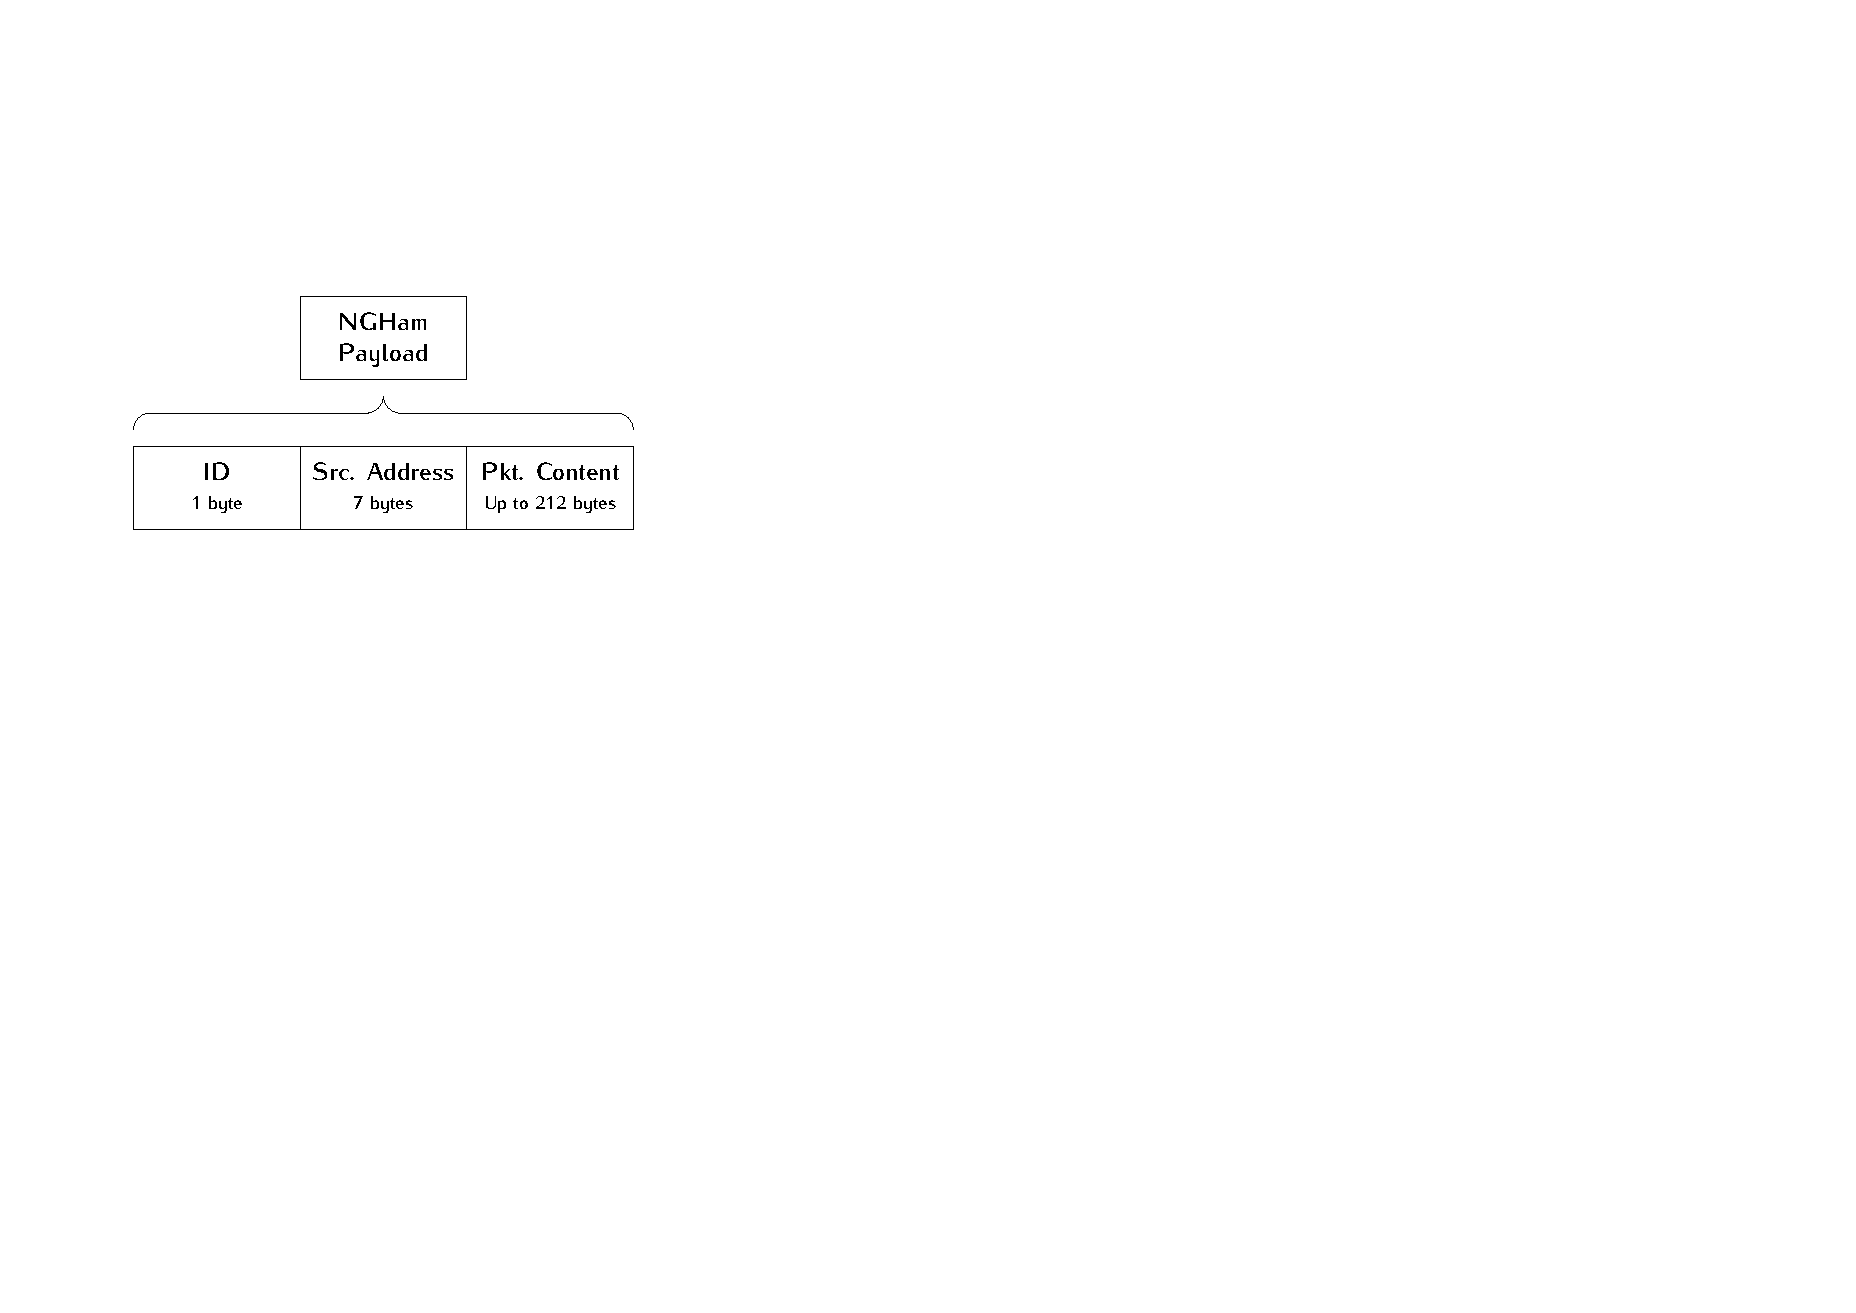
\includegraphics[width=0.5\textwidth]{figures/floripasat-packet-structure.pdf}
        \caption{Payload structure of the FloripaSat-2 packets.}
        \label{fig:fsat-pkt-structure}
    \end{center}
\end{figure}

The \autoref{tab:packets-struct} summarizes all types of packets transmitted or received by the satellite, with the ID number, the structure and length of and the access type of each packet.

\begin{landscape}
    \begin{table}[ht]
        \centering
        \begin{tabular}{llccccc}
            \toprule[1.5pt]
            \multirow{2}{*}{\textbf{Link}} & \multirow{2}{*}{\textbf{Packet Name}} & \multicolumn{4}{c}{\textbf{Payload}} & \multirow{2}{*}{\textbf{Access}} \\
            \cmidrule{3-6}
                                      &                       & \textbf{ID}  & \textbf{Source Callsign}   & \textbf{Data (up to 220 bytes)}            & \textbf{Size (bytes)} & \\
            \midrule
            \multirow{2}{*}{Beacon}   & EPS data              & 00h & \multirow{2}{*}{`` '' + ``PY0EFS''} & EPS data                                   & 58                    & Public \\
                                      & TTC Data              & 01h &                                     & TTC data                                   & 18                    & Public \\
            \midrule
            \multirow{6}{*}{Downlink} & General telemetry     & 20h & \multirow{6}{*}{`` '' + ``PY0EFS''} & OBDH/EPS data                              & 75                    & Public \\
                                      & Ping answer           & 21h &                                     & Requester callsign                         & 15                    & Public \\
                                      & Data request answer   & 22h &                                     & Requester callsign + data                  & 15 to 155             & Public \\
                                      & Message broadcast     & 23h &                                     & Requester + dst. callsign + message        & 22 to 60              & Public \\
                                      & Payload data          & 24h &                                     & Payload ID + payload data                  & 9 to 220              & Public \\
                                      & TC feedback           & 25h &                                     & Req. callsign + TC packet ID + timestamp   & 13                    & Public \\
            \midrule
            \multirow{12}{*}{Uplink}  & Ping request          & 40h & \multirow{12}{*}{Any Callsign}      & None                                       & 8                     & Public \\
                                      & Data request          & 41h &                                     & Data flags + count + origin + offset       & 16                    & Public \\
                                      & Broadcast Message     & 42h &                                     & Dst. callsign + message                    & 15 to 46              & Public \\
                                      & Enter hibernation     & 43h &                                     & Req. callsign + hibernation in hours + key & 29                    & Private \\
                                      & Leave hibernation     & 44h &                                     & TC key                                     & 16                    & Private \\
                                      & Activate module       & 45h &                                     & Module ID + TC key                         & 17                    & Private \\
                                      & Deactivate module     & 46h &                                     & Module ID + TC key                         & 17                    & Private \\
                                      & Activate payload      & 47h &                                     & Payload ID + TC key                        & 17                    & Private \\
                                      & Deactivate payload    & 48h &                                     & Payload ID + TC key                        & 17                    & Private \\
                                      & Erase memory          & 49h &                                     & TC key                                     & 16                    & Private \\
                                      & Force reset           & 4Ah &                                     & TC key                                     & 16                    & Private \\
                                      & Get payload data      & 4Bh &                                     & Payload ID + TC key + payload args.        & 17 to 28              & Private \\
            \bottomrule[1.5pt]
        \end{tabular}
        \caption{Telecommunication packets and their content.}
        \label{tab:packets-struct}
    \end{table}
\end{landscape}

The ID of the modules that can be activated or deactivated are available in \autoref{tab:module-id}.

\begin{table}[ht]
    \centering
    \begin{tabular}{lcL{0.53\textwidth}c}
        \toprule[1.5pt]
        \textbf{Module} & \textbf{ID Number} \\
        \midrule
        Battery heater      & 1 \\
        Beacon              & 2 \\
        Periodic telemetry  & 3 \\
        \bottomrule[1.5pt]
    \end{tabular}
    \caption{IDs of the modules that can be activated or deactivated.}
    \label{tab:module-id}
\end{table}

The ID of the payloads, to be used in the activate/deactivate telecommands, are available in \autoref{tab:payload-id}.

\begin{table}[ht]
    \centering
    \begin{tabular}{lc}
        \toprule[1.5pt]
        \textbf{Payload} & \textbf{ID Number} \\
        \midrule
        EDC 1               & 1 \\
        EDC 2               & 2 \\
        Payload-X           & 3 \\
        Radiation monitor   & 4 \\
        \bottomrule[1.5pt]
    \end{tabular}
    \caption{IDs of the payloads.}
    \label{tab:payload-id}
\end{table}

\begin{table}[ht]
    \centering
    \begin{tabular}{lcL{0.53\textwidth}c}
        \toprule[1.5pt]
        \textbf{Packet} & \textbf{Position} & \textbf{Content} & \textbf{Length [bytes]} \\
        \midrule
        \multirow{22}{*}{EPS data} & 0  & Packet ID (00h)                       & 1 \\
                                   & 1  & Source callsign (`` PY0EFS'')         & 7 \\
                                   & 8  & Timestamp in ms                       & 4 \\
                                   & 12 & Battery cell 1 voltage in mV          & 2 \\
                                   & 14 & Battery cell 2 voltage in mV          & 2 \\
                                   & 16 & Battery current in mA                 & 2 \\
                                   & 18 & Battery charge in mAh                 & 2 \\
                                   & 20 & Battery cell 1 temperature in K       & 2 \\
                                   & 22 & Battery cell 2 temperature in K       & 2 \\
                                   & 24 & Battery monitor temperature in K      & 2 \\
                                   & 26 & Solar panel voltage in mV (-Y and +X) & 2 \\
                                   & 28 & Solar panel voltage in mV (-X and +Z) & 2 \\
                                   & 30 & Solar panel voltage in mV (-Z and +Y) & 2 \\
                                   & 32 & Solar panel current in mA (-Y)        & 2 \\
                                   & 34 & Solar panel current in mA (+Y)        & 2 \\
                                   & 36 & Solar panel current in mA (-X)        & 2 \\
                                   & 38 & Solar panel current in mA (+X)        & 2 \\
                                   & 40 & Solar panel current in mA (-Z)        & 2 \\
                                   & 42 & Solar panel current in mA (+Z)        & 2 \\
                                   & 44 & Temperature of the EPS $\mu$C in K    & 2 \\
        \cmidrule{4-4}
                                   &    &                                       & 46 \\
        \midrule
        \multirow{9}{*}{TTC data}  & 0  & Packet ID (01h)                       & 1 \\
                                   & 1  & Source callsign (`` PY0EFS'')         & 7 \\
                                   & 8  & Timestamp in ms                       & 4 \\
                                   & 12 & Temperature of the TTC $\mu$C in K    & 2 \\
                                   & 14 & Reset counter                         & 2 \\
                                   & 16 & Last reset cause                      & 1 \\
                                   & 15 & Temperature of the beacon radio in K  & 2 \\
        \cmidrule{4-4}
                                   &    &                                       & 19 \\
        \bottomrule[1.5pt]
    \end{tabular}
    \caption{Beacon packets.}
    \label{tab:beacon-packets}
\end{table}

\begin{longtable}[c]{lcL{0.4\textwidth}c}
    \toprule[1.5pt]
    \textbf{Packet} & \textbf{Position} & \textbf{Content} & \textbf{Length [bytes]} \\
    \midrule
    \multirow{42}{*}{General telemetry}     & 0  & Packet ID (20h)                              & 1 \\
                                            & 1  & Source callsign (`` PY0EFS'')                & 7 \\
                                            & 8  & Time counter in milliseconds                 & 4 \\
                                            & 12 & Temperature of the OBDH $\mu$C in Kelvin     & 2 \\
                                            & 14 & Input current of the OBDH in mA              & 2 \\
                                            & 16 & Input voltage of the OBDH in mV              & 2 \\
                                            & 18 & Last reset cause of the OBDH                 & 1 \\
                                            & 19 & Reset counter of the OBDH                    & 2 \\
                                            & 21 & Last valid telecommand (uplink packet ID)    & 1 \\
                                            & 22 & Temperature of the radio in Kelvin           & 2 \\
                                            & 24 & RSSI of the last valid telecommand           & 2 \\
                                            & 26 & Temperature of the antenna in Kelvin         & 2 \\
                                            & 28 & Antenna status                               & 2 \\
                                            & 30 & Payloads status                              & 1 \\
                                            & 31 & Temperature of the EPS $\mu$C in K           & 2 \\
                                            & 33 & EPS circuitry and Beacon MCU current in mA   & 2 \\
                                            & 35 & Last reset cause of the EPS                  & 1 \\
                                            & 36 & Reset counter (EPS)                          & 2 \\
                                            & 38 & -Y and +X sides solar panel voltage in mV    & 2 \\
                                            & 40 & -X and +Z sides solar panel voltage in mV    & 2 \\
                                            & 42 & -Z and +Y sides solar panel voltage in mV    & 2 \\
                                            & 44 & -Y side solar panel current in mA            & 2 \\
                                            & 46 & +Y side solar panel current in mA            & 2 \\
                                            & 48 & -X side solar panel current in mA            & 2 \\
                                            & 50 & +X side solar panel current in mA            & 2 \\
                                            & 52 & -Z side solar panel current in mA            & 2 \\
                                            & 54 & +Z side solar panel current in mA            & 2 \\
                                            & 55 & MPPT 1 duty cycle in \%                      & 1 \\
                                            & 56 & MPPT 2 duty cycle in \%                      & 1 \\
                                            & 57 & MPPT 3 duty cycle in \%                      & 1 \\
                                            & 59 & Main power bus voltage in mV                 & 2 \\
                                            & 61 & Batteries voltage in mV                      & 2 \\
                                            & 63 & Batteries current in mA                      & 2 \\
                                            & 65 & Batteries average current in mA              & 2 \\
                                            & 67 & Batteries accumulated current in mA          & 2 \\
                                            & 69 & Batteries charge in mAh                      & 2 \\
                                            & 71 & Battery monitor IC temperature in K          & 2 \\
                                            & 73 & Battery heater 1 duty cycle in \%            & 1 \\
                                            & 74 & Battery heater 2 duty cycle in \%            & 1 \\
                                            & 75 & Payload EDC status (00h=none, 01h=EDC\_1, 02h=EDC\_2, 03h=Both) & 1 \\
                                            & 76 & Payload-X status (00h=OFF,01h=ON)            & 1 \\
                                            & 77 & Radiation monitor status (00h=OFF,01h=ON)    & 1 \\
    \cmidrule{4-4}
                                            &    &                                              & 78 \\
    \multirow{3}{*}{Ping answer}            & 0  & Packet ID (21h)                      & 1 \\
                                            & 1  & Source callsign (`` PY0EFS'')        & 7 \\
                                            & 8  & Requester callsign                   & 7 \\
    \cmidrule{4-4}
                                            &    &                                      & 15 \\
    \multirow{3}{*}{Data request answer}    & 0  & Packet ID (22h)                      & 1 \\
                                            & 1  & Source callsign (`` PY0EFS'')        & 7 \\
                                            & 8  & Requester callsign                   & 7 \\
    \cmidrule{4-4}
                                            &    &                                      & 15 \\
    \multirow{5}{*}{Message broadcast}      & 0  & Packet ID (23h)                      & 1 \\
                                            & 1  & Source callsign (`` PY0EFS'')        & 7 \\
                                            & 8  & Requester callsign                   & 7 \\
                                            & 15 & Destination callsign                 & 7 \\
                                            & 22 & Message                              & up to 38 \\
    \cmidrule{4-4}
                                            &    &                                      & 22 to 60 \\
                                            & 0  & Packet ID (24h)                      & 1 \\
                                            & 1  & Source callsign (`` PY0EFS'')        & 7 \\
                                            & 8  & Payload ID (01h or 02h)              & 1 \\
                                            & 9  & PTT signal receiving time            & 4 \\
                                            & 13 & Error code                           & 1 \\
                                            & 14 & Carrier frequency                    & 2 \\
                                            & 16 & Carrier amplitude at ADC interface output & 2 \\
                                            & 18 & User message length in bytes         & 1 \\
                                            & 19 & ARGOS-2 PTT-A2 user message          & 35 \\
                                            & 54 & Current time since J2000 epoch       & 4 \\
                                            & 58 & Elapsed time since last reset        & 4 \\
   Payload data                             & 62 & System current supply in mA          & 2 \\
   (EDC info)                               & 64 & System voltage supply in mV          & 2 \\
                                            & 65 & EDC board temperature                & 1 \\
                                            & 66 & RF front end LO                      & 1 \\
                                            & 67 & RMS level at front-end output        & 2 \\
                                            & 69 & Generated PTT packages since last initialization & 1 \\
                                            & 70 & Max                                  & 1 \\
                                            & 71 & Memory error count                   & 1 \\
                                            & 72 & Current time                         & 4 \\
                                            & 76 & Number of PTT package available for reading & 1 \\
                                            & 77 & PTT decoder task status              & 1 \\
                                            & 78 & ADC sampler state                    & 1 \\
    \cmidrule{4-4}
                                            &    &                                      & 79 \\
                                            & 0  & Packet ID (24h)                      & 1 \\
                                            & 1  & Source callsign (`` PY0EFS'')        & 7 \\
                                            & 8  & Payload ID (01h or 02h)              & 1 \\
                                            & 9  & Elapsed time since J2000 epoch       & 4 \\
    Payload data                            & 13 & ADC sample packet number             & 1 \\
    (EDC samples)                           & 14 & First ADC I-sample                   & 2 \\
                                            & 16 & First ADC Q-sample                   & 2 \\
                                            & ... & ...                                 & ... \\
                                            & 214 & N ADC I-sample                      & 2 \\
                                            & 216 & N ADC Q-sample                      & 2 \\
    \cmidrule{4-4}
                                            &    &                                      & 218 \\
    \multirow{5}{*}{TC feedback}            & 0  & Packet ID (25h)                      & 1 \\
                                            & 1  & Source callsign (`` PY0EFS'')        & 7 \\
                                            & 8  & Requester callsign                   & 7 \\
                                            & 15 & TC packet ID                         & 1 \\
                                            & 16 & Timestamp                            & 4 \\
    \cmidrule{4-4}
                                            &    &                                      & 20 \\
    \bottomrule[1.5pt]
    \caption{Downlink packets.}
    \label{tab:downlink-packets}
\end{longtable}

\begin{longtable}[c]{lcL{0.4\textwidth}c}
    \toprule[1.5pt]
    \textbf{Packet} & \textbf{Position} & \textbf{Content} & \textbf{Length [bytes]} \\
    \midrule
    \multirow{2}{*}{Ping request}       & 0  & Packet ID (40h)                      & 1 \\
                                        & 1  & Ground station callsign              & 7 \\
    \cmidrule{4-4}
                                        &    &                                      & 8 \\
    \multirow{2}{*}{Data request}       & 0  & Packet ID (41h)                      & 1 \\
                                        & 1  & Ground station callsign              & 7 \\
    \cmidrule{4-4}
                                        &    &                                      & 8 \\
    \multirow{4}{*}{Broadcast message}  & 0  & Packet ID (42h)                      & 1 \\
                                        & 1  & Ground station callsign              & 7 \\
                                        & 8  & Destination callsign                 & 7 \\
                                        & 15 & Message                              & up to 38 \\
    \cmidrule{4-4}
                                        &    &                                      & up to 53 \\
    \multirow{4}{*}{Enter hibernation}  & 0  & Packet ID (43h)                      & 1 \\
                                        & 1  & Ground station callsign              & 7 \\
                                        & 8  & Hibernation in hours                 & 2 \\
                                        & 10 & TC key                               & 8 \\
    \cmidrule{4-4}
                                        &    &                                      & 18 \\
    \multirow{3}{*}{Leave hibernation}  & 0  & Packet ID (44h)                      & 1 \\
                                        & 1  & Ground station callsign              & 7 \\
                                        & 8  & TC key                               & 8 \\
    \cmidrule{4-4}
                                        &    &                                      & 16 \\
    \multirow{4}{*}{Activate module}    & 0  & Packet ID (45h)                      & 1 \\
                                        & 1  & Ground station callsign              & 7 \\
                                        & 8  & Module ID                            & 1 \\
                                        & 9  & TC key (one for each module)         & 8 \\
    \cmidrule{4-4}
                                        &    &                                      & 17 \\
    \multirow{4}{*}{Deactivate module}  & 0  & Packet ID (46h)                      & 1 \\
                                        & 1  & Ground station callsign              & 7 \\
                                        & 8  & Module ID                            & 1 \\
                                        & 9  & TC key (one for each module)         & 8 \\
    \cmidrule{4-4}
                                        &    &                                      & 17 \\
    \multirow{4}{*}{Activate payload}   & 0  & Packet ID (47h)                      & 1 \\
                                        & 1  & Ground station callsign              & 7 \\
                                        & 8  & Payload ID                           & 1 \\
                                        & 9  & TC key (one for each payload)        & 8 \\
    \cmidrule{4-4}
                                        &    &                                      & 17 \\
    \multirow{4}{*}{Deactivate payload} & 0  & Packet ID (48h)                      & 1 \\
                                        & 1  & Ground station callsign              & 7 \\
                                        & 8  & Payload ID                           & 1 \\
                                        & 9  & TC key (one for each payload)        & 8 \\
    \cmidrule{4-4}
                                        &    &                                      & 17 \\
    \multirow{3}{*}{Erase memory}       & 0  & Packet ID (49h)                      & 1 \\
                                        & 1  & Ground station callsign              & 7 \\
                                        & 8  & TC key                               & 8 \\
    \cmidrule{4-4}
                                        &    &                                      & 16 \\
    \multirow{3}{*}{Force reset}        & 0  & Packet ID (4Ah)                      & 1 \\
                                        & 1  & Ground station callsign              & 7 \\
                                        & 8  & TC key                               & 8 \\
    \cmidrule{4-4}
                                        &    &                                      & 16 \\
    \multirow{3}{*}{Get payload data}   & 0  & Packet ID (4Bh)                      & 1 \\
                                        & 1  & Ground station callsign              & 7 \\
                                        & 8  & Payload ID                           & 1 \\
                                        & 9  & TC key (one for each payload)        & 8 \\
                                        & 17 & Payload arguments                    & up to 11 \\
    \cmidrule{4-4}
                                        &    &                                      & 16 \\
    \bottomrule[1.5pt]
    \caption{Uplink packets.}
    \label{tab:uplink-packets}
\end{longtable}

\subsection{Operation Licenses}

.

    %
% subsystems.tex
%
% Copyright (C) 2021 by SpaceLab.
%
% FloripaSat-2 Documentation
%
% This work is licensed under the Creative Commons Attribution-ShareAlike 4.0
% International License. To view a copy of this license,
% visit http://creativecommons.org/licenses/by-sa/4.0/.
%

%
% \brief Subsystems chapter.
%
% \author Gabriel Mariano Marcelino <gabriel.mm8@gmail.com>
%
% \institution Universidade Federal de Santa Catarina (UFSC)
%
% \version 0.1.0
%
% \date 2020/06/06
%

\chapter{Subsystems} \label{ch:subsystems}

This chapter presents a description of all subsystems of the space segment of the mission, which can be seen in the exploded view of the satellite, available in \autoref{fig:exploded-view}.

\begin{figure}[!ht]
    \begin{center}
        \includegraphics[width=\textwidth]{figures/exploded-view}
        \caption{Exploded view of the FloripaSat-2 satellite.}
        \label{fig:exploded-view}
    \end{center}
\end{figure}

Most of the subsystems presented here have their own documentation, with a deeper technical description of it. When available, there is a reference to the respective document. This chapter is intended to show an overview of each subsystem, in a macro context of the mission.

\section{On-Board Data Handling}

The OBDH\nomenclature{\textbf{OBDH}}{\textit{On-Board Data Handling}.} 2.0 is an On-Board Computer (OBC) module designed for nanosatellites. The module is responsible for synchronizing actions and the data flow between other modules (i.e., power module, communication module, payloads) and the Earth segment. It packs the generated data into data frames and transmit back to Earth through a communication module, or stores it on a non-volatile memory for later retrieval. Commands sent from Earth segment to the CubeSat are received by radio transceivers located in the communication module and redirected to the OBDH, which takes the appropriate action or forward the commands to the target module.

The module is a direct upgrade from the OBDH of FloripaSat-1 \cite{floripasat}, which grants a flight heritage rating. The improvements focus on providing a cleaner and more generic implementation in comparison with the previous version, more reliability in software and hardware implementations, and adaptations for the new mission requirements. The board of the module can be seen in \autoref{fig:obdh2}.

\begin{figure}[!ht]
    \begin{center}
        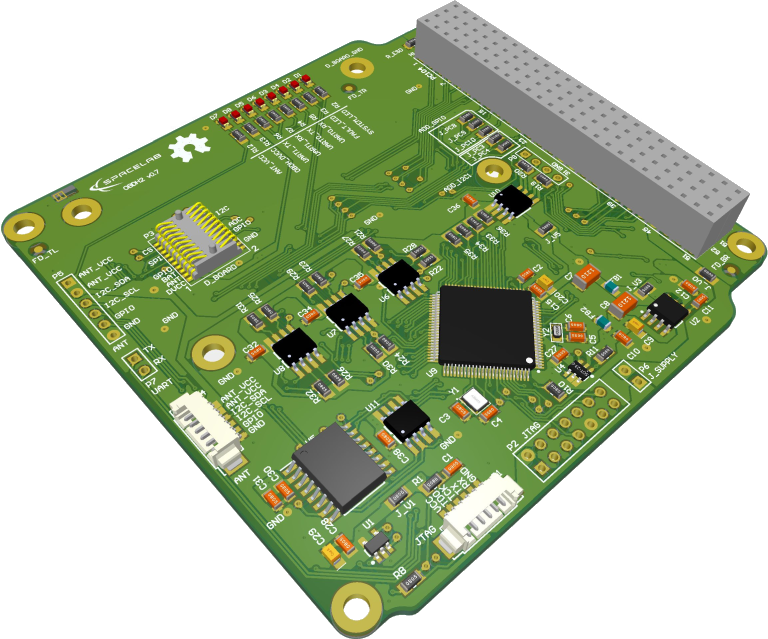
\includegraphics[width=0.7\textwidth]{figures/obdh2-pcb-3d}
        \caption{OBDH module.}
        \label{fig:obdh2}
    \end{center}
\end{figure}

More information about this module can be found in \cite{obdh2}.

\section{Telemetry, Tracking and Command Module}

The TTC\nomenclature{\textbf{TTC}}{\textit{Telemetry, Tracking and Command Module}.} (or TT\&C) is responsible to make the communication between the earth (a ground station) and the satellite, and is divided in two sub-modules: Beacon and downlink/uplink. The beacon is a independent sub-module who transmits a periodic signal containing an identification data (ID) of the satellite and some basic telemetry data. The downlink/uplink sub-module is the main communication device. It has a bidirectional data link to receive telecommands from the earth and transmit all available data back to Earth. The board of the module can be seen in \autoref{fig:ttc}.

\begin{figure}[!ht]
    \begin{center}
        \includegraphics[width=0.7\textwidth]{figures/ttc_board}
        \caption{TTC module.}
        \label{fig:ttc}
    \end{center}
\end{figure}

More information about this module can be found in \cite{ttc}.

\subsection{Antenna Module}

The used antenna module is the CubeSat deployable VHF and UHF antenna from ISISpace \cite{isis-antenna}. It is a four monopole antenna built with tape strings (up to 55 cm) and compliant with the CubeSat standard (dipole or turnstile options are also available). The deployment method is the burning wire and it can be controlled digitally through a I$^{2}$C interface. To allow redundancy, there are two independent deployment controllers that can be activated separately. Also, the construction of this module allows the installation of a solar panel at the top side. The RF gain is about 0 dBi.

A picture of the antenna module (with all antennas released) can be seen in \autoref{fig:isis-antenna}.

\begin{figure}[!ht]
    \begin{center}
        \includegraphics[width=0.8\textwidth]{figures/isis-antenna}
        \caption{Antenna module from ISISpace.}
        \label{fig:isis-antenna}
    \end{center}
\end{figure}

The chosen configuration for this mission can be seen below (using \autoref{fig:isis-antenna-ref} as reference):

\begin{itemize}
    \item Configuration: 4 monopoles (1x VHF + 3x UHF)
        \begin{itemize}
            \item Antenna 1: VHF - 145,97 MHz (beacon)
            \item Antenna 2: UHF - 401,635 MHz (EDC)
            \item Antenna 3: UHF - 436,9 MHz (downlink/uplink)
            \item Antenna 4: UHF - 401,635 MHz (redundant EDC)
        \end{itemize}
    \item Tuning structure size: 2U
    \item Mounting position: Top
    \item Supply voltage: 3,3 V
    \item I$^{2}$C control type: Dual bus
        \begin{itemize}
            \item Primary I$^{2}$C address: 31h (7-bit address)
            \item Redundant I$^{2}$C address: 32h (7-bit address)
        \end{itemize}
    \item I$^{2}$C watchdog: Enabled with a time out of 60 seconds.
\end{itemize}

\begin{figure}[!ht]
    \begin{center}
        \includegraphics[width=0.7\textwidth]{figures/isis-antenna-ref}
        \caption{Configuration reference of the antenna module.}
        \label{fig:isis-antenna-ref}
    \end{center}
\end{figure}

In the digital interface, a temperature sensor and the state of four deployment switches (1 per monopole) are also available. These switches indicate if a monopole is released or not, and can be used as feedback of the deployment process.

\section{Electrical Power System}

The EPS\nomenclature{\textbf{EPS}}{\textit{Electrical Power System}.} is the module designed to harvest, store and distribute energy for the satellite. The energy harvesting system is based on solar energy conversion through te solar panels attached to the CubeSat structure. The EPS is designed to operate the solar panels at their maximum power point (MPPT\nomenclature{\textbf{MPPT}}{\textit{Maximum Power Point Tracking}.}). The board also measures the solar panels current, voltage and the temperature of the batteries. The harvested solar energy is stored in a battery module connected to the EPS. The energy distribution is done by several integrated buck DC-DC converters. The full EPS system is composed of the solar panels, the EPS PCB\nomenclature{\textbf{PCB}}{\textit{Printed Circuit Board.}} and the battery module. A general view of the EPS board can be seen in \autoref{fig:eps2}.

\begin{figure}[!ht]
    \begin{center}
        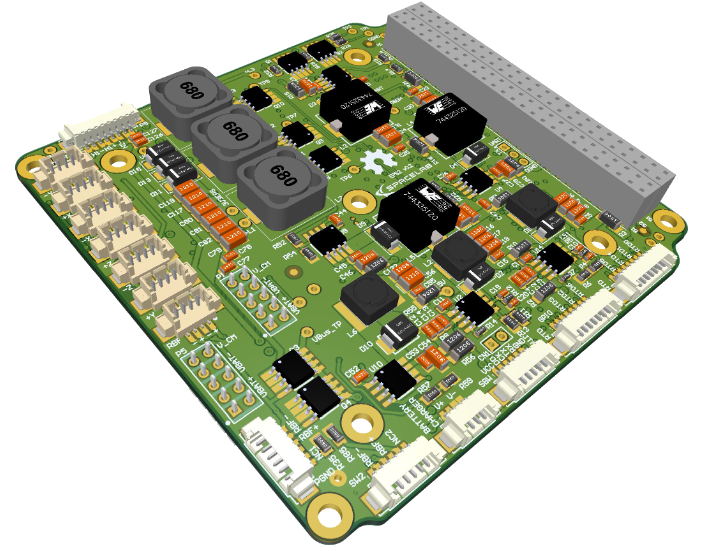
\includegraphics[width=0.7\textwidth]{figures/eps2-pcb-3d}
        \caption{EPS module.}
        \label{fig:eps2}
    \end{center}
\end{figure}

The module is a direct upgrade from the EPS of FloripaSat-1 \cite{floripasat}, which grants a flight heritage rating. The improvements focus on providing a cleaner and more generic implementation in comparison with the previous version, more reliability in software, and adaptations for the new mission requirements.

More information about this module can be found in \cite{eps2}.

\subsection{Battery Module}

The used battery module is the ``\textit{Battery Module 4C}'', that is a separate battery module from the EPS board and composed by four lithium-ion 18650 cells. Besides the cells, the board has connectors for interfacing signals and power lines with the EPS module, 2 power resistors to operate as heaters to maintain the cell's temperature during eclipse periods, and 4 temperature sensors. The batteries used are the ICR18650-30B lithium-ion cells from Samsung \cite{icr18650-30b}, which are connected in series and parallel (two sets of two parallel cells in series) to supply the required voltage and current. Each cell is fixed with 18650 metal holders and between the pairs there is the power resistor attached with a thermal element in the middle. A mechanical mount is placed over the batteries and screwed to the board, providing better stress resistance. Also, there are PC-104 through hole pads present on the board for a connector that could be used for making mechanical integration with the EPS, or with future improvements a interface for power, data or control signals. The board is a direct improvement from the first battery board used in the FloripaSat-1 mission \cite{floripasat}.

\begin{figure}[!ht]
    \begin{center}
        \includegraphics[width=0.7\textwidth]{figures/bat2-pcb-3d}
        \caption{Battery module board.}
        \label{fig:battery-module-board}
    \end{center}
\end{figure}

More information about the battery module can be found in \cite{bat4c}.

\subsection{Solar Panels}

The solar panels are a set of 5 custom made panels manufactured by ORBITAL, a Brazilian company, and a single panel from ISISpace. The panels features protection diodes and high-efficiency solar cells, which are the CESI's CTJ-30 \cite{ctj30} with dimensions 6,9 $\times$ 3,9 cm (area 26,5 cm$^{2}$). This cell is qualified for space use by ESA with an efficiency of 29,5 \% (AM0, BOL). The panels do not include magnetorquers, sensors and others devices. The top solar panel is a model from ISISpace to ensure mechanical compatibility with the antenna module (also from ISISpace). These two types of solar panels can be seen in Figures \ref{fig:solar-panel-orbital} and \ref{fig:top-solar-panel}.

\begin{figure}[!ht]
    \begin{center}
        \includegraphics[width=0.7\textwidth]{figures/orbital-solar-panel}
        \caption{Conceptual solar panel from ORBITAL.}
        \label{fig:solar-panel-orbital}
    \end{center}
\end{figure}

\begin{figure}[!ht]
    \begin{center}
        \includegraphics[width=0.6\textwidth]{figures/isis-top-solar-panel}
        \caption{Top solar panel from ISISpace.}
        \label{fig:top-solar-panel}
    \end{center}
\end{figure}

\subsection{Kill-Switches and RBF}

Two electronic switches have been implemented into the design as to allow for the (redundant) deployment detection of the CubeSat when it is deployed from the POD. This electronic microswitch can be used to prevent the satellite from starting up during launch as is required for all CubeSat launches and hence acts as a Kill-Switch. The Kill-Switch is the Panasonic AV4 microswitch (AV402461), as can be seen in \autoref{fig:av402461}.

\begin{figure}[!ht]
    \begin{center}
        \includegraphics[width=0.25\textwidth]{figures/av402461}
        \caption{Panasonic AV402461 Microswitch.}
        \label{fig:av402461}
    \end{center}
\end{figure}

The Kill-Switch mechanism in the mechanical structure has combined the function of providing deployment and detection (\autoref{fig:kill-switch-installed}). The travel of the actual switch of the Kill-Switch itself is so short that the Kill-Switch could ``detect deployment'' of the CubeSat from the launch adapter simply due to launch vibrations. To overcome this issue the Kill-Switch has been rotated so that there is a positive obstruction in front of the switch which needs 8 mm of deployment before deployment can be detected with the Kill-Switch. In \autoref{fig:kill-switch-installed} the Kill-Switch parts are highlighted and the stowed and deployed configuration is shown.

\begin{figure}[!ht]
    \begin{center}
        \includegraphics[width=0.85\textwidth]{figures/kill-switch-installed}
        \caption{Kill-Switches installed in the mechanical structure.}
        \label{fig:kill-switch-installed}
    \end{center}
\end{figure}

The contact arrangement of the microswitch and the current rating are detailed in \autoref{fig:circuit-kill-switch} and \autoref{tab:kill-switch-specs}.

\begin{figure}[!ht]
    \begin{center}
        \includegraphics[width=0.4\textwidth]{figures/circuit-kill-switch}
        \caption{The contact arrangement of the microswitch.}
        \label{fig:circuit-kill-switch}
    \end{center}
\end{figure}

\begin{table}[!h]
    \centering
    \begin{tabular}{lcccc}
        \toprule[1.5pt]
        \textbf{Characteristic} & \textbf{Minimum} & \textbf{Typical} & \textbf{Maximum} & \textbf{Unit} \\
        \midrule
        Switch Current                      & 2     & 50    & 100   & mA \\
        DC Voltage across switch contacts   & n/a   & n/a   & 30    & V \\
        Contact resistance microswitch      & n/a   & n/a   & 200   & m$\Omega$ \\
        \bottomrule[1.5pt]
    \end{tabular}
    \caption{Kill-Switch current rating and voltage range.}
    \label{tab:kill-switch-specs}
\end{table}

\section{Attitude Control System}

The Attitude Control System (ACS\nomenclature{\textbf{ACS}}{\textit{Attitude Control System}.}) is a passive attitude control system, which depends on the Earth's magnetic field to rotate and stabilize the satellite \cite{santoni2009,gerhardt2010}. The system is composed of one permanent magnet to create a force to align the magnet with the Earth's magnetic field and four hysteresis bars to damp the cube oscillations and achieve stabilization.

When equilibrium is achieved, the permanent magnet aligns itself to the Earth's field lines. The hysteresis bars convert oscillation and rotation energy into heat, maintaining the alignment through magnetic moment. The components are placed in positions as to minimize the magnet's interaction with the hysteresis bars, which limits the magnetic moment of the magnet \cite{francois2010}. \autoref{fig:adcs} shows the mounting of the hysteresis bars (green) and the permanent magnet (red) on the mechanical structure. The whole passive ACS was implemented according to \cite{francois2010}.

\begin{figure}[!ht]
    \begin{center}
        \includegraphics[width=0.7\textwidth]{figures/adcs}
        \caption{ACS subsytem. Rare earth magnet (pink) and hysteresis bars (red) installed in the structure.}
        \label{fig:adcs}
    \end{center}
\end{figure}

As a passive magnetic attitude control system is used, it is possible to stabilize only one axis, and so, the CubeSat will still slowly (due to hysteresis bars) rotate around this axis, even after stabilized. A N45 neodymium magnet and 4 hysteresis bars of Permanorm 5000 H2 are used (courtesy of Vacuumschmelze GmbH \& Co. KG). The material of the hysteresis bar is shaped in order to maximize the stabilization, which is the most important part of the attitude control.

Many conditions impact on the detumbling time, which is the time required for the satellite to stabilize. Magnetic passive attitude stabilization systems such as the one developed for this mission achieve the equilibrium state within a few weeks of operation \cite{santoni2009}.

The FloripaSat-2 satellite does not feature an orbit control subsystem.

\section{Mechanical Structure}

The USIPED 2-Unit CubeSat structure is developed as a generic, modular satellite structure based upon the CubeSat standard. The modular chassis allows for up to two 1-Unit stack of PCBs, or other modules, to be mounted inside the chassis, using the PC-104 standard and spacers attached to the structure. In addition, there are 4 slots in the middle section, providing space for the interface boards and the ACS. The solar panels and antennas are externally mounted, providing a complete mechanical solution. A picture of this structure can be seen in \autoref{fig:usiped-structure}.

\begin{figure}[!ht]
    \begin{center}
        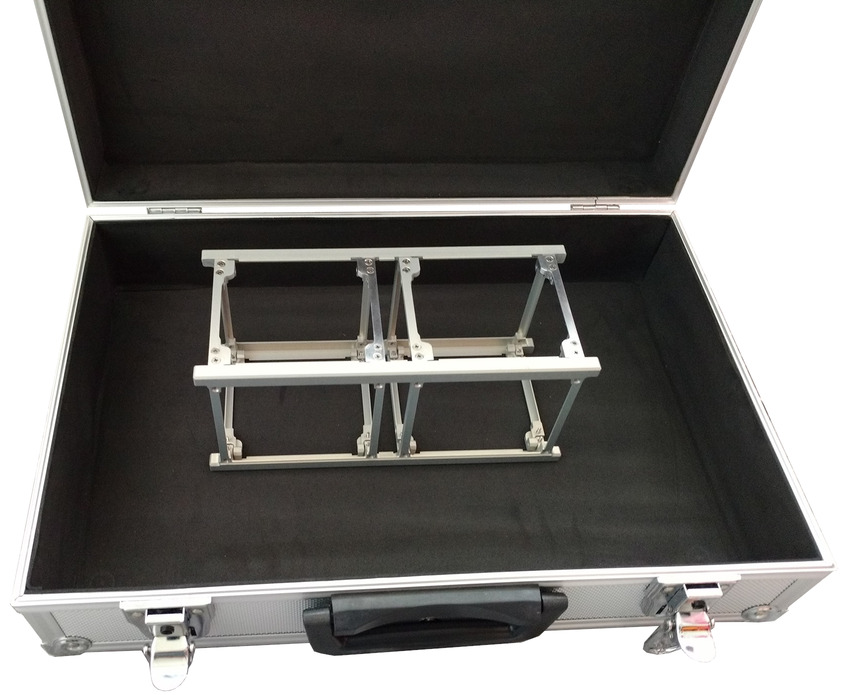
\includegraphics[width=0.7\textwidth]{figures/usiped-2u-structure.jpg}
        \caption{2U CubeSat structure from Usiped.}
        \label{fig:usiped-structure}
    \end{center}
\end{figure}

\section{Interconnection Modules}

\subsection{PC-104 Interconnection Boards}

The PC-104 interconnection boards are intended to be used as an interconnection of the two PC-104 bus segments of the 2U structure (top and bottom units). This interconnection is made with a set of PicoBlade cables between the top and bottom boards. The set of two boards can be seen in \autoref{fig:pc104-adapter}.

\begin{figure}[!ht]
    \begin{center}
        \includegraphics[width=0.7\textwidth]{figures/pc104-adapter}
        \caption{PC-104 adapter boards (top and bottom).}
        \label{fig:pc104-adapter}
    \end{center}
\end{figure}

More information about these boards can be found in \cite{pc104-boards}.

\subsection{External Connection Boards}

The Interstage Interface Panels (IIP) are three vertical internally mounted PCBs designed to give external access up to four modules inside of a 2U CubeSat during final assembly, integration and testing (AIT) before launch. The complete set of the boards allow the nanosatellite to be charged, programed and debugged. The usage of this hardware platform is taking into account the use of a MSP-FET: MSP430 Flash Emulation Tool from Texas Instruments for JTAG programing and debugging, UART debugging through a mini USB type B port interfacing the FT4232H USB bridge IC from FTDI, a JST XH header for charging internal batteries and a Remove Before Flight (RBF) pin header. The boards can seen in \autoref{fig:iip-boards}.

\begin{figure}[!ht]
    \begin{center}
        \includegraphics[width=0.7\textwidth]{figures/iip_fullset}
        \caption{Set of external connection boards.}
        \label{fig:iip-boards}
    \end{center}
\end{figure}

More information about these boards can be found in \cite{iip}.

\section{Payloads}

The FloripaSat-2 satellite is planned to carry three different payloads on-board: ``\textit{EDC}'', ``\textit{Payload-X}'' and the ``\textit{Harsh Payload}''. Each one of these payloads are presented next.

\subsection{Environmental Data Collection}

The Environmental Data Collector (EDC\nomenclature{\textbf{EDC}}{\textit{Environmental Data Collection}.}) is a CubeSat-compatible payload that decodes signals from Platform Transmitter Terminals (PTTs) belonging to the Brazilian Environmental Data Collection System (SBCD\nomenclature{\textbf{SBCD}}{\textit{Sistema Brasileiro de Coleta de Dados}.}) and the Argos-2 System. It is the main payload of the FloripaSat-2 mission.

The main featues of this payload are listed below, a 3D model of the EDC board can be seen in \autoref{fig:edc-board}.

\begin{itemize}
    \item Reception/decoding of SBCD and Argos-2 signals on the 401.635 MHz $\pm$ 30 kHz frequency range.
    \item Can decode up to 12 PTT signals simultaneously.
    \item Attaches a header to decoded messages with frequency, time, and signal strength information.
    \item Full speed I$^{2}$C interface (400 kbit/s) for the OBC communication.
    \item Full-duplex RS-485 interface with fail-safe for the OBC communication.
    \item 5 V power supply.
    \item Memory capable of storing up to 64 decoded user messages.
    \item Generates housekeeping information including current supply, board temperature, digitized signal RMS level, front-end PLL synchronism state and overcurrent events.
    \item Can capture a 2048 samples sequence (16 ms window) from the received signal upon request.
\end{itemize}

\begin{figure}[!ht]
    \begin{center}
        \includegraphics[width=0.6\textwidth]{figures/edc-pcb-top}
        \caption{EDC board.}
        \label{fig:edc-board}
    \end{center}
\end{figure}

As can be seen in \autoref{fig:exploded-view}, for this mission, two identical EDC boards will be used, in a cold redundancy configuration. More information about this payload can be found in \cite{edc}.

\subsection{Redundant OBDH (Payload-X)}

The Payload-X is a radiation-hardened reconfigurable hardware platform designed for a radioactive environment, having as a main feature the possibility to change the hardware configuration of the FPGA\nomenclature{\textbf{FPGA}}{\textit{Field-Programmable Gate Array.}} through remote uplink of its bitstream.

\begin{figure}[!ht]
    \begin{center}
        \includegraphics[width=0.6\textwidth]{figures/payload-x-board}
        \caption{Payload-X board.}
        \label{fig:payload-x-board}
    \end{center}
\end{figure}

More information about this payload can be found in \cite{rigo2019}.

\subsection{Radiation Monitor (Harsh Payload)}

The Radiation Monitor (or Harsh Payload) is a payload capable of evaluate the radiation effects on three SDRAM\nomenclature{\textbf{SDRAM}}{\textit{Synchronous Dynamic Random-Access Memory.}} memories with different manufacturing nodes. This payload will test this chips in the real harsh space environment by flying aboard of FloripaSat-2 CubeSat mission. These particular SDRAM memories were previous characterized on laboratory experiments, then by exposing them to the real environments and executing the same tests routines will not only generate more results for analysis, but also provide an opportunity to assess the test methodologies themselves. Also, after collecting sufficient data to be analysed, this payload could be used to provide a meaningful health status, concerning the radiation doses which the satellite were exposed, to the entire satellite subsystems and further missions. A picture of the harsh payload board is available in \autoref{fig:harsh-payload}.

\begin{figure}[!ht]
    \begin{center}
        \includegraphics[width=0.7\textwidth]{figures/harsh-payload}
        \caption{Radiation monitor board. Top (left) and bottom (right) sides.}
        \label{fig:harsh-payload}
    \end{center}
\end{figure}

In order to accomplish this objectives, the payload is designed to follow the OBDH DaughterBoard standard of SpaceLab, which defines the connectors, shape and size of the board. This standard allows the utilization of the module throughout future SpaceLab core missions in reason of its low space occupation inside the CubeSat, being considered further as an expansion module instead of a payload experiment. A picture of the exploded view of the harsh payload and the OBDH can be seen in \autoref{fig:harsh-payload-integration}.

\begin{figure}[!ht]
    \begin{center}
        \includegraphics[width=0.7\textwidth]{figures/daughterboard-integration}
        \caption{Integration of the radiation monitor payload in the OBDH.}
        \label{fig:harsh-payload-integration}
    \end{center}
\end{figure}

Also, due to the mission limited power budget, the developed board should consider reduce power consumption and define clever power management strategies. In addition, methods for anti latch-up, a type of short circuit which can occur inside an IC, are considered in the design. Therefore, combining all these requirements, the payload architecture consists of the following modules: a control and management subsystem, operated by a System-On-a-Chip (SoC\nomenclature{\textbf{SoC}}{\textit{System-On-a-Chip.}}) solution with an integrated FPGA, power converters for properly voltage level supply, anti latch-up circuitry, communication and interface buses, debug module and the SDRAM memory chips.

    %
% ground_segment.tex
%
% Copyright (C) 2021 by SpaceLab.
%
% GOLDS-UFSC Documentation
%
% This work is licensed under the Creative Commons Attribution-ShareAlike 4.0
% International License. To view a copy of this license,
% visit http://creativecommons.org/licenses/by-sa/4.0/.
%

%
% \brief Ground segment chapter.
%
% \author Gabriel Mariano Marcelino <gabriel.mm8@gmail.com>
%
% \institution Universidade Federal de Santa Catarina (UFSC)
%
% \version 0.1.0
%
% \date 2020/06/06
%

\chapter{Ground Segment} \label{ch:ground-segment}

\section{Hardware}

.

\section{Satellite Tracking}

To track the satellite and for orbit prediction, the GPredict software \cite{gpredict} will be used.

A picture of the main window of GPredict can be seen in \autoref{fig:gpredict}.

\begin{figure}[!ht]
    \begin{center}
        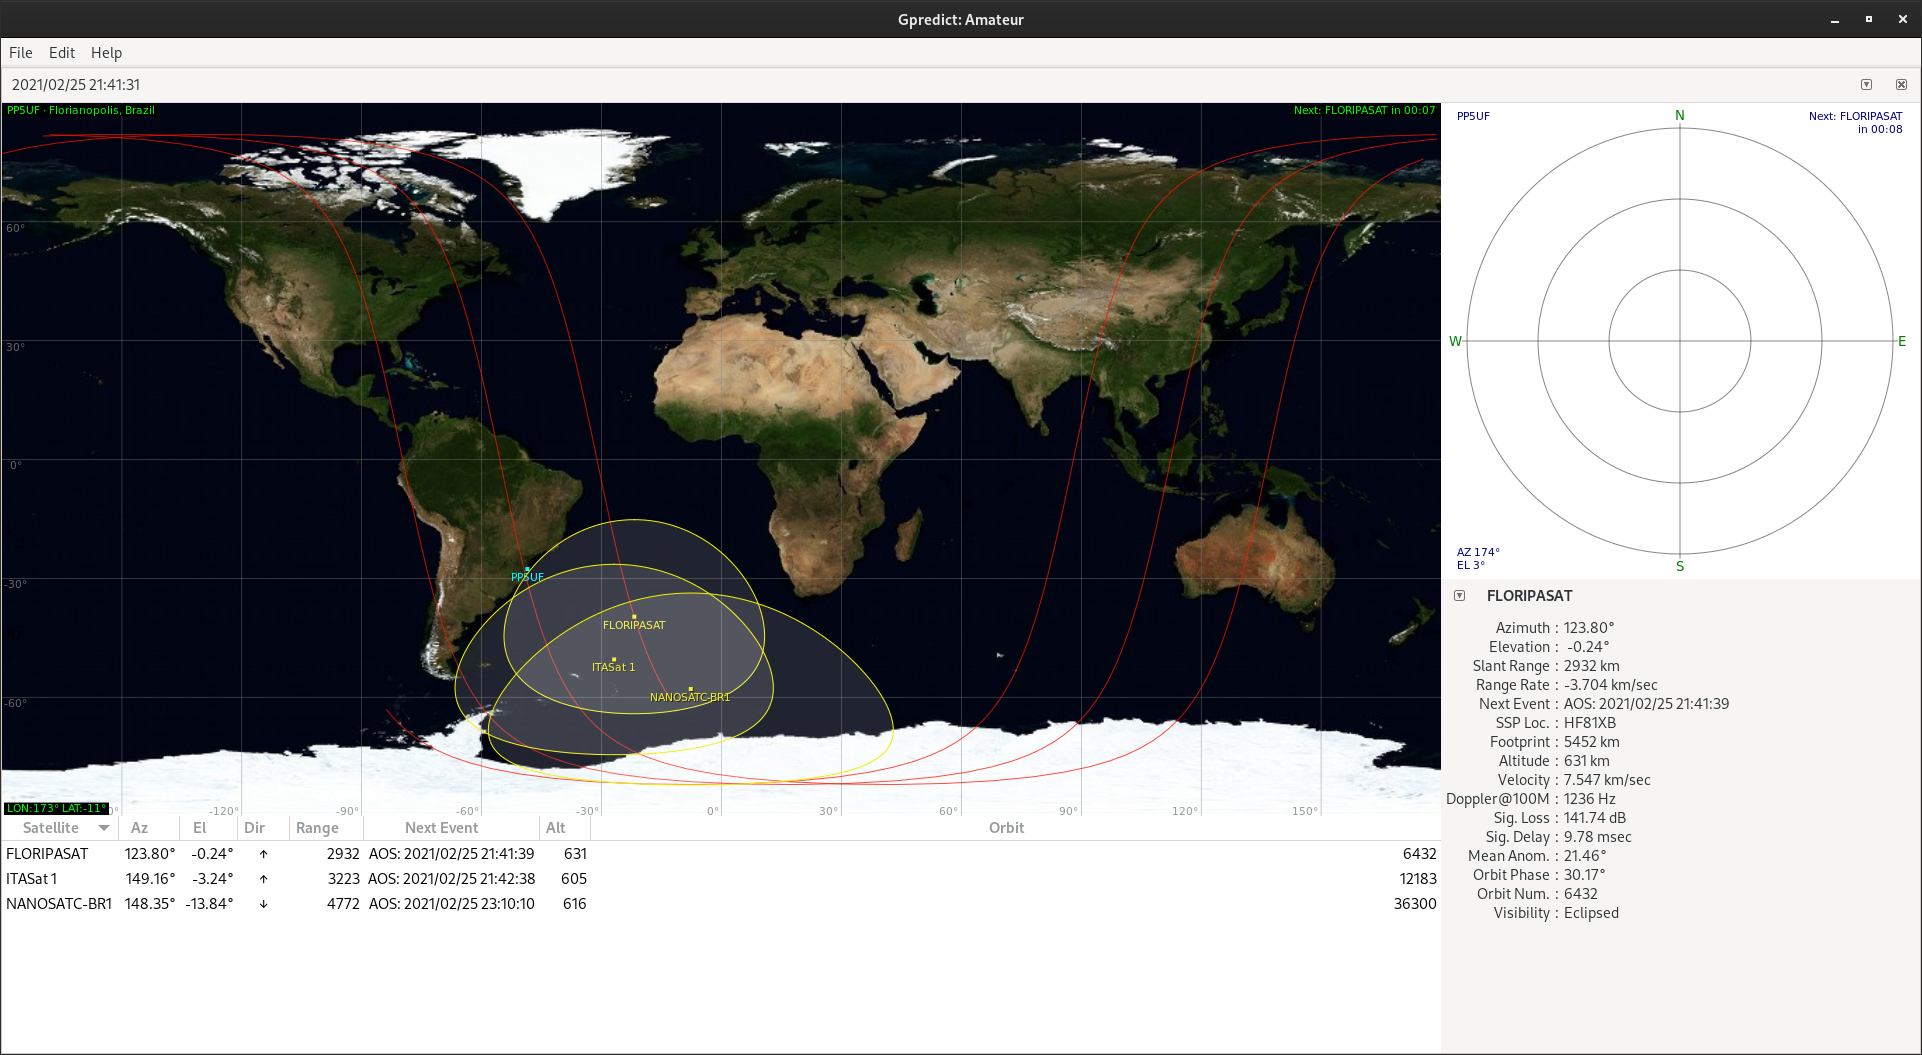
\includegraphics[width=\textwidth]{figures/gpredict.png}
        \caption{Main window of GPredict.}
        \label{fig:gpredict}
    \end{center}
\end{figure}

    %
% tests.tex
%
% Copyright (C) 2021 by SpaceLab.
%
% FloripaSat-2 Documentation
%
% This work is licensed under the Creative Commons Attribution-ShareAlike 4.0
% International License. To view a copy of this license,
% visit http://creativecommons.org/licenses/by-sa/4.0/.
%

%
% \brief Test plan and results.
%
% \author Gabriel Mariano Marcelino <gabriel.mm8@gmail.com>
%
% \institution Universidade Federal de Santa Catarina (UFSC)
%
% \version 0.1.0
%
% \date 2021/01/21
%

\chapter{Test Plan and Results} \label{ch:test-plan}

The FloripaSat-2 test plan is structured into four phases: Module tests, FlatSat, Engineering integration, and Flight integration. This plan is summarized in the \autoref{tab:test-plan} and includes the components under test for each phase. 

\begin{table}[!h]
    \begin{center}
        \begin{tabular}{ll}
            \toprule[1.5pt]
            \textbf{Phase}    & \textbf{Components}       \\
            \midrule
            Module tests             & OBDH module \\
                                     & EPS module \\
                                     & TTC module \\
                                     & BATC4 board \\
                                     & IIP boards \\
                                     & PC104-ADPT boards \\
                                     & ACS components (simulation) \\
                                     & Mechanical (CAD assessment) \\
            \midrule
            FlatSat                  & Satellite core (OBDH+EPS+TTC+BATC4) \\
                                     & Satellite core + GRS \\
                                     & Satellite core + Payloads \\
                                     & Satellite core + Payloads + GRS \\
                                     & Satellite (long-term evaluation) \\
            \midrule
            Engineering integration  & Mechanical assembly (repeated when required) \\
            (clean room preferable)  & Satellite core + Payloads + GRS \\
                                     & Satellite (long-term evaluation) \\
                                     & Satellite + Solar Panels \\
                                     & Preliminary environmental tests \\ 
            \midrule
            Flight integration       & Mechanical assembly (flight components) \\
            (clean room mandatory)   & Satellite (short-term evaluation) \\
                                     & Satellite + Antenna (deployment) \\
                                     & Mechanical reassembly for flight \\
                                     & Satellite (long-term evaluation) \\
                                     & Qualification environmental tests \\ 
            \bottomrule[1.5pt]
        \end{tabular}
        \caption{Test plan phases and tested components.}
        \label{tab:test-plan}
    \end{center}
\end{table}

This section focus on providing an overview of the planned testing workflow and a description of the strategies approached to accomplish the mission objectives. The module tests focus on the individual modules operation and behavior, in which a general template is provided in this document and each module applies it for their needs. The FlatSat phase is the first modules integration in a debug platform to validate the system from a development perspective (described with more details in \cite{flatsat}). Finally, the engineering integration is the final development campaign aiming to validate the system from a mission perspective and the flight integration is the actual CubeSat assembly using the flight components and final assessments to prepare the satellite for launch. The integration details, procedures and qualification proccess are described with more depth in the \autoref{ch:ait}. % maybe it will be splitted in a separated document

\section{Module tests}

The first phase is the foundation for the satellite, consolidating the base design for each subsystem and shaping their relations. Therefore, several techniques were employed to ensure a solid test strategy: several inspections of the boards design and manufacturing quality; manual experimental assessments of various hardware electrical, mechanical and behavioral parameters; remotely automated tests using a continuos integration (CI)\nomenclature{\textbf{CI}}{\textit{Continuos Integration.}} approach; semi-automated tests using a hardware-in-the-loop (HIL)\nomenclature{\textbf{HIL}}{\textit{Hardware-In-the-Loop.}} strategy; simulations; and CAD models assessment.

\subsection{Workflow}

The following topics lists the template workflow used to create the procedures for each subsystem. Each module documentation has its own test chapter describing the process in detail, from procedures to success criteria.

% \item [\footnotesize{XX-00}] Text 
\subsubsection{Visual Inspection} 
\begin{enumerate} \setlength\itemsep{-0.3em}
    \item Packaging quality assessment
    \item Board manufacturing and assembly quality
    \item 3D model comparison
    \item Layers marker
    \item Labels (schematics comparison) 
    \item High resolution photos for documentation
\end{enumerate}

\subsubsection{Mechanical Inspection}
\begin{enumerate} \setlength\itemsep{-0.3em}
    \item Board dimensions and mounting holes positioning
    \item Board weight measurement
\end{enumerate}

\subsubsection{Integration Inspection}
\begin{enumerate} \setlength\itemsep{-0.3em}
    \item Check connectors pinout against the documentation (not schematics)
    \item Check connectors positioning (if applicable)
\end{enumerate}

\subsubsection{Electrical Inspection}
\begin{enumerate} \setlength\itemsep{-0.3em}
    \item Solder shorts
    \item Missing components
    \item Lifted pins
    \item Poor soldering
    \item Swapped components
    \item Components partnumber
    \item Components polarity (schematic comparison)
    \item Components defined to not be soldered (DNP)
\end{enumerate}

\subsubsection{Electrical Testing}
\begin{enumerate} \setlength\itemsep{-0.3em}
    \item Continuity test
    \item Power up procedures (check LEDs and testpoints)
    \item Average input power consumption measurement
    \item Average output power source measurement (if applicable) 
    \item Power tracks temperature (if applicable)
    \item Simple signal integrity (if applicable)
\end{enumerate}

\subsubsection{Functional Testing}
\begin{enumerate} \setlength\itemsep{-0.3em}
    \item Run a simple test code (if applicable) 
    \item Run the system code (if applicable and available) 
    \item Check the system hardware self-test flags (if applicable and available) 
    \item Monitor basic LEDs behavior (if applicable) 
    \item Monitor the debug serial port logs (if applicable)
\end{enumerate}

\subsubsection{Module Testing}
\begin{enumerate} \setlength\itemsep{-0.3em}
    \item Run simulations and review results (if applicable)
    \item Review operation behavior against the documentation (if applicable)
    \item Review features and requirements fulfillment
    \item Review communication buses configuration and protocol (if applicable)
    \item Review data packages, power buses and control signals
    \item Review and evaluate operation edge cases
    \item Run remote automated code tests (if applicable)
    \item Run system test codes in the board (if applicable)
    \item Run latest stable code version, monitor logs and qualify behavior (if applicable)
\end{enumerate}


\subsection{Continuos Integration}

In order to detect errors and bugs in the early stages of development, a continuos integration workflow was setup for automated firmware tests focusing in small scope verfications (i.e., unit tests). Instead of executing the code in the target processor, the tests are executed remotely in a host computer through the usage of an unit testing framework, called "cmocka" \textcolor{red}{cite cmocka}. This tool allows to abstract the inherent hardware dependencies of embedded systems to enable firmware tests without errors introduced by hardware problems (exection in a consolidated platform, the computer), which provides an optimal behavioral assessment of the code implementations. This approach not only support remote testing, but promote continuos test execution, which is essencial to detect erros and architectural issues. The integration of these procedures is powered by "GitHub Actions" \textcolor{red}{cite GH Action}, which provides a host machine and a dashboard inside the same environment of the already used version control, source distribution and management tool.

The unit tests follows a layered structure accordingly with the firmware layers. This is used alongside mockups (i.e., interfaces that abstract what the layer receive as input without having to implement the underlying functionality), which allows independency between the layers and abstract the actual hardware dependencies with an emulated behavior.


\subsection{Hardware-In-the-Loop}



\subsubsection{Integration Tests}

\begin{itemize} \setlength\itemsep{-0.3em}
    \item Operating system initialization: assert memory allocation (RAM, stack, heap), hooks and etc;
    \item Boot sequence (as similar to the actual procedure as possible).
    \item Operating system task/queue/interrupts priority, constraints, size, depth and delay checks: use dummy task/queue/interrupts (same config as actual system).
    \item Short-term system check: after 1 hour, exit without error logs.
    \item Mid-term system check: after 1 day, exit without error logs.
    \item Long-term system check (used in flatsat): after 1 week, exit without flatsat/integration error logs.
\end{itemize}

\subsubsection{Workflow}

\begin{itemize} \setlength\itemsep{-0.3em}
    \item Always it is a build->flash->test, change main and repeat.
    \item It must have a test folder containing subfolders (hardware, drivers, devices, app, integration) and a json file (with name, path and type).
    \item Inside the workflow is called a python script that read this json and setup variables to allow running multiple main file swaps for each test type.
    \item There are 5 different workflows, one for each test type: hardware, drivers, devices, app, integration;
    \item The workflow, tests and scripts must be reviewed before each release.
    \item Idea: for short/mid/long-term tests, the workflow should evaluate the log messages offline instead of real time, in which a job is scheduled to run just after this period and ``a script'' will read the log file and search for the test criteria, giving the actual CI result.
    \item Idea: Inside the code, using the log message approach, we might create our ultra lightweight framework that consists of only log types (colors) and log messages (specific strings). This way we do not modify our current workflow and we can add a simple scheme to access the flight code.
    \item Unit Tests = Tests performed per firmware unit.
    \item Integration Tests = Tests performed per firmware component (several units abstracted).
\end{itemize}



\section{Flatsat}

To test all modules during the development of the projet, a flatsat platform was developed. The FlatSat Platform is a testbed for CubeSat PCB modules. FlatSats enable easier, faster and a secure method for testing subsystens independently while been integrated in a flat design before going to integration on a CubeSat form factor. The PCB can support up to 7 modules, all PC-104 pins are interligated to flexibilize its use, only the particularity connection between modules need to be be taken into account. One PC-104 has inverted pinout, the board also makes it possible to have two seperate power supplies, a UART to USB converter for 4 modules, kill-switches activation though SPDTs, Remove Before Flight (RBF) pin header, connector for charging batteries and SMA connectors for antennas. A picture of the flatsat board can be seen in \autoref{fig:flatsat-top}.

\begin{figure}[!ht]
    \begin{center}
        \includegraphics[width=\textwidth]{figures/flatsat_top_image}
        \caption{Top view of the flatsat board.}
        \label{fig:flatsat-top}
    \end{center}
\end{figure}

More information about the Flatsat Platform can be found in \cite{flatsat}.




\subsection{Environmental Tests}

LIT\nomenclature{\textbf{LIT}}{\textit{Laboratório de Integração e Testes.}}

\cite{marcelino2021}

\subsubsection{Mass Verification}

This test checks the total mass of the satellite (without RBF tag), which must be less than 2,66 kg \cite{cds}. The verification is made with a precision balance. \autoref{fig:mass-verification} examplifies this process with FloripaSat-I total mass.

\begin{figure}[!ht]
    \begin{center}
        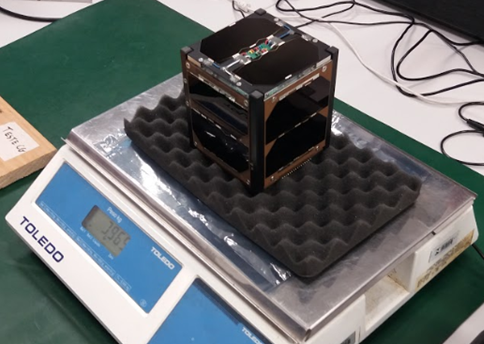
\includegraphics[width=0.5\textwidth]{figures/mass-test}
        \caption{Mass verificatiton of FloripaSat-I.}
        \label{fig:mass-verification}
    \end{center}
\end{figure}

\subsubsection{Center of Gravity}

This test checks the center of gravity (CG) of the satellite, which must be less than 2 cm from the geometric center (see \autoref{fig:cg}) \cite{cds}. To perform this test, a simple test-bench based on two parallel bars fixed on a plate (4 cm from each other) can be used. The geometric center of the satellite is put in the middle of the bars and, if the satellite does not fall, the CG is within the radius of 2 cm. This strategy does not measure the location of CG, however, it does prove if the satellite follows the requirement.

\begin{figure}[!htb]
    \begin{center}
        \subfigure[$X$ axis.\label{fig:fsat-fm-x-axis}]{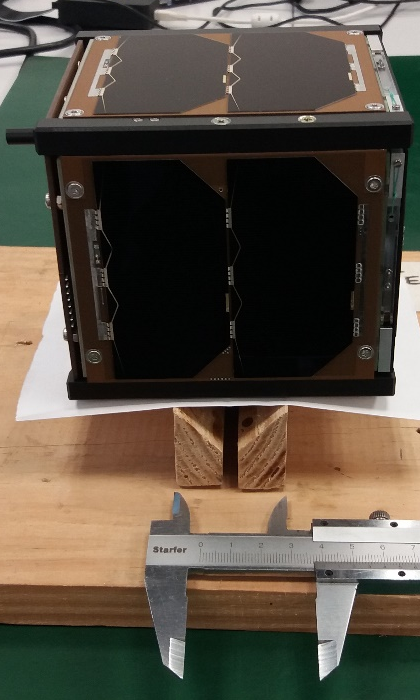
\includegraphics[width=0.2\textwidth]{figures/fsat_fm_x_axis.png}}
        ~
        \subfigure[$Y$ axis.\label{fig:fsat-fm-y-axis}]{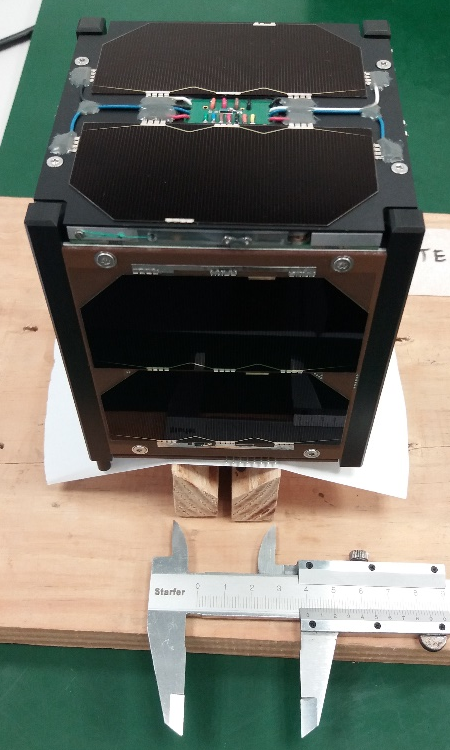
\includegraphics[width=0.2\textwidth]{figures/fsat_fm_y_axis.png}}
        ~
        \subfigure[$Z$ axis.\label{fig:fsat-fm-z-axis}]{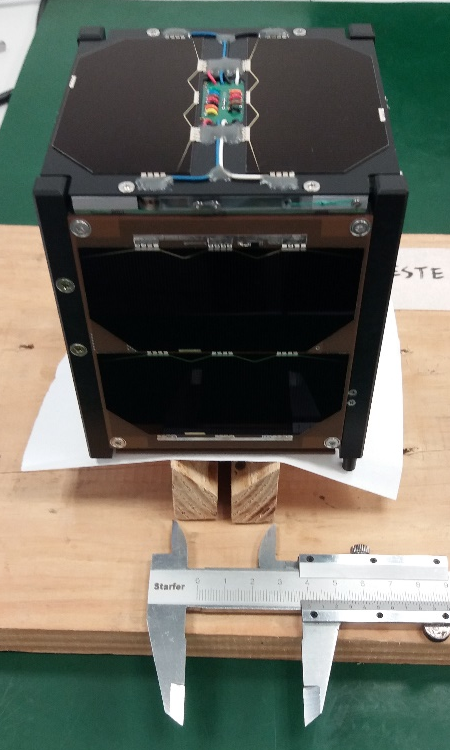
\includegraphics[width=0.2\textwidth]{figures/fsat_fm_z_axis.png}}
        \caption{Center of gravity of FloripaSat-I within 2 cm from geometric center.}
        \label{fig:cg}
    \end{center}
\end{figure}

\subsubsection{Vibration Test}

To measure and control the acceleration profile during the dynamic tests, accelerometers should be positioned on three external surfaces of the satellite, one on each axis, over areas without solar cells. The satellite should be fixed on a shaker. Figure \ref{fig:fsat-vibration-accel} shows some of the accelerometers and Figure \ref{fig:fsat-shaker} shows the satellite during a vibration test.

\begin{figure}[!htb]
    \begin{center}
        \subfigure[Position of the accelerometers.\label{fig:fsat-vibration-accel}]{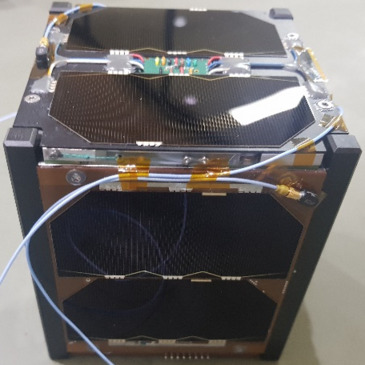
\includegraphics[height=4.5cm]{figures/fsat_fm_accel.jpg}}
        ~
        \subfigure[Shaker.\label{fig:fsat-shaker}]{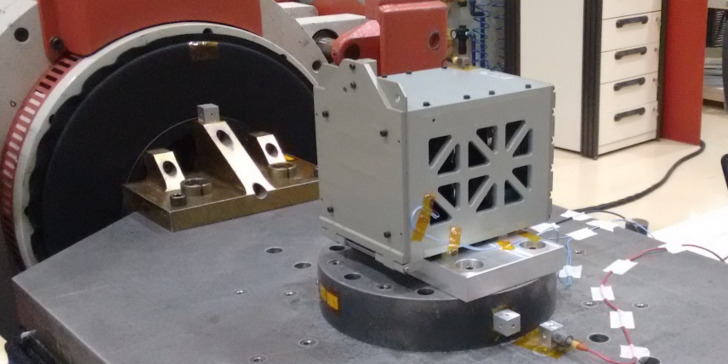
\includegraphics[height=4.5cm]{figures/fsat_fm_shaker.jpg}}
        \caption{Vibration test.}
        \label{fig:vibration-test}
    \end{center}
\end{figure}

The CubeSat should be tested entirely off, with RBF pin removed but with the Kill-Switches pressed, in a 2U Test POD, simulating the normal launching condition. The set of vibration tests follows \autoref{fig:vibration_procedure}.

\begin{figure}[!ht]
    \begin{center}
        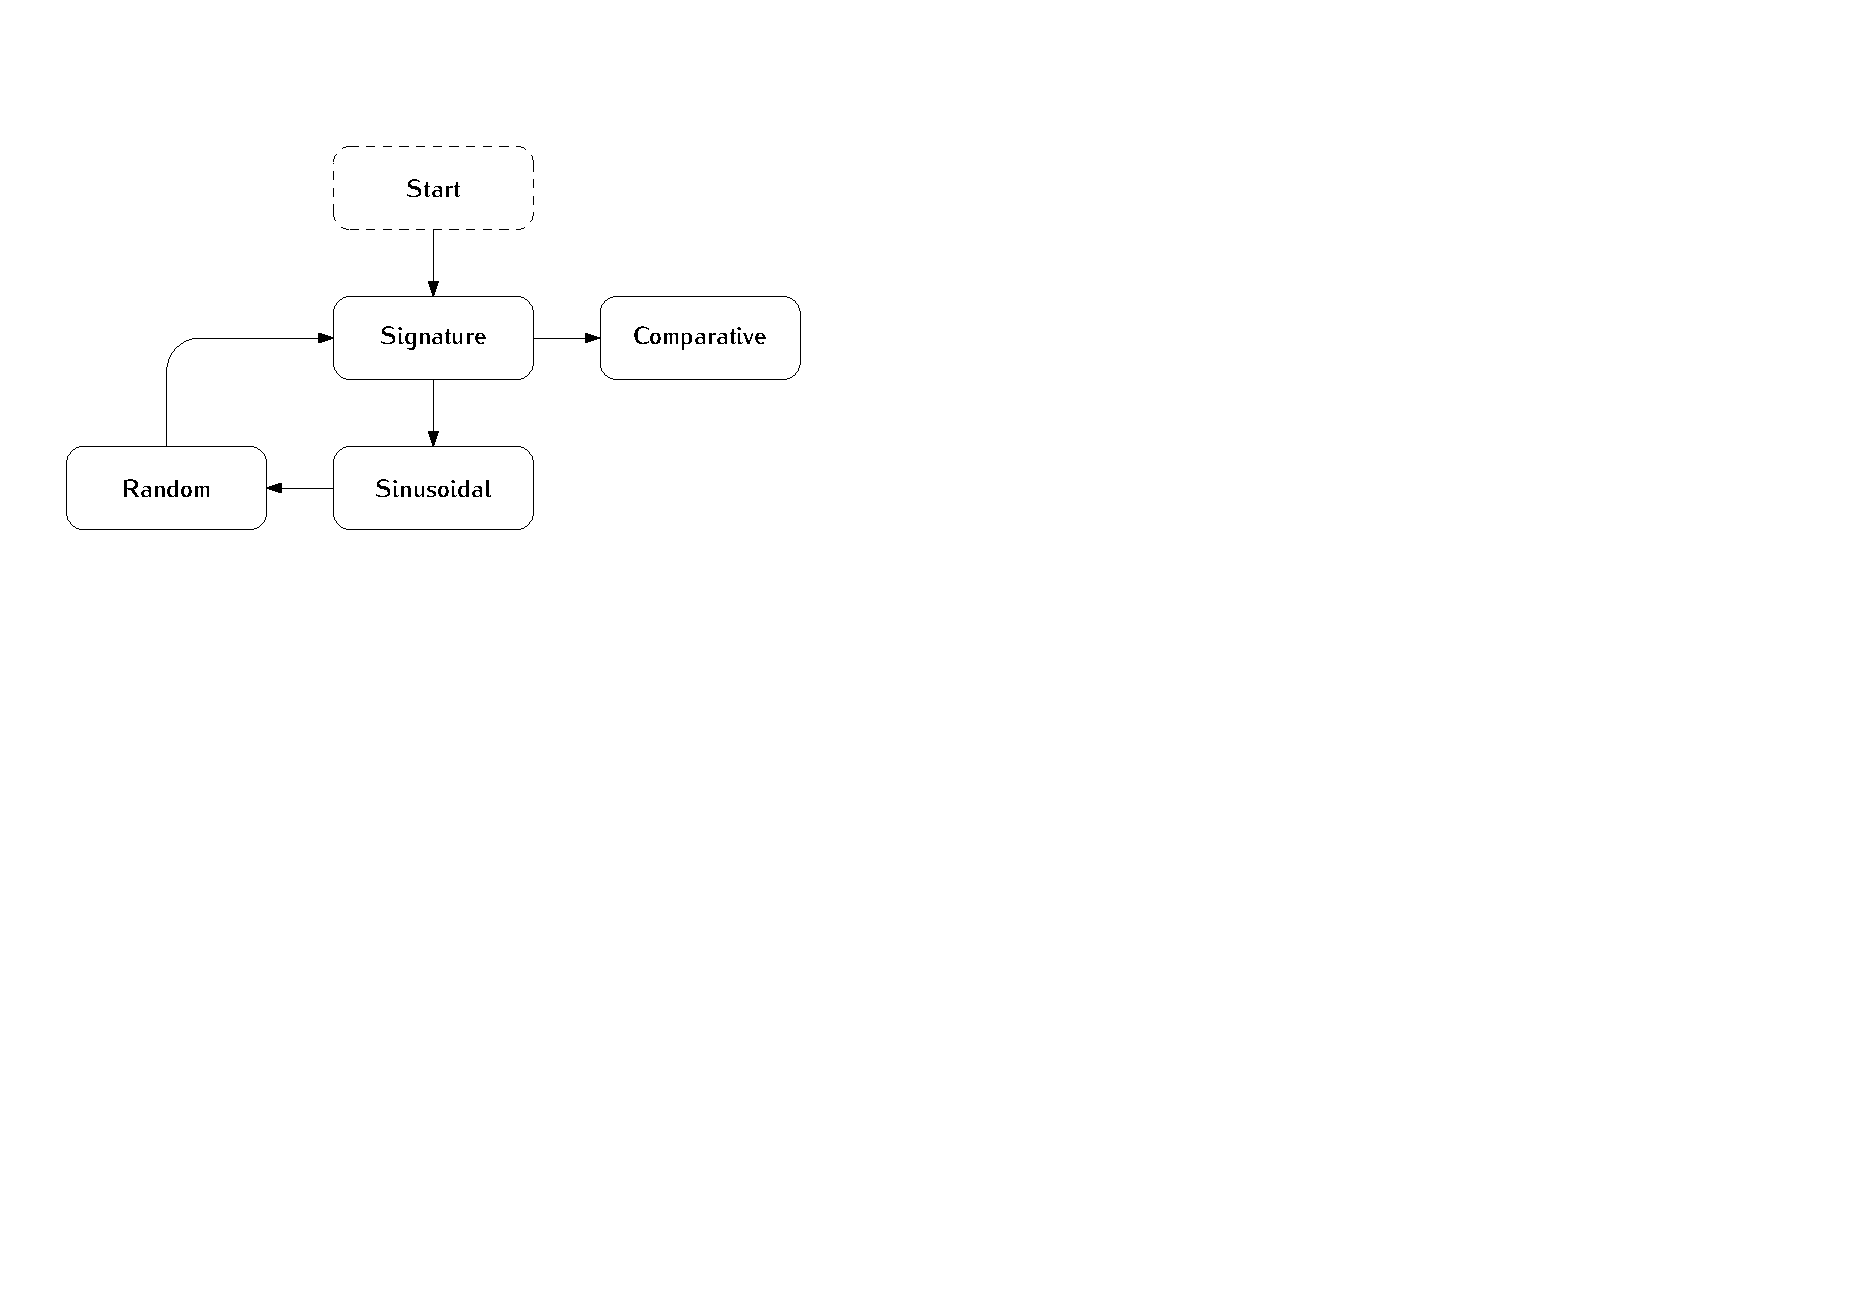
\includegraphics[width=0.6\textwidth]{figures/vibration_procedure.pdf}
        \caption{Sequence of dynamic tests.}
        \label{fig:vibration_procedure}
    \end{center}
\end{figure}

A signature testing should be conducted before and after the tests (sinusoidal and random vibration), in order to identify the presence of significant variations in the dynamic response, a condition that may represent mechanical failures. For the signature task, \autoref{tab:vibration-test-dynamic-1} presents the specifications.

\begin{table}[!h]
    \begin{center}
        \begin{tabular}{ll}
            \toprule[1.5pt]
            \textbf{Name}    & \textbf{Parameter}       \\
            \midrule
            Test method      & Sinusoidal sweep testing \\
            Frequency range  & 5 - 2000 Hz              \\
            Vibration level  & 0,25 g                   \\
            Sweep rate       & 2 octaves per minute     \\
            Number of sweeps & 1 (5 - 2000 Hz)          \\
            Test axes        & 3 ($X$, $Y$, $Z$)        \\
            \bottomrule[1.5pt]
        \end{tabular}
        \caption{Resonance survey test (signature).}
        \label{tab:vibration-test-dynamic-1}
    \end{center}
\end{table}

%Regarding the sinusoidal sweeping vibration, Table 3 brings the envelope of the test, and so does Fig. 24 in a graphic format.

\begin{figure}[!ht]
    \begin{center}
        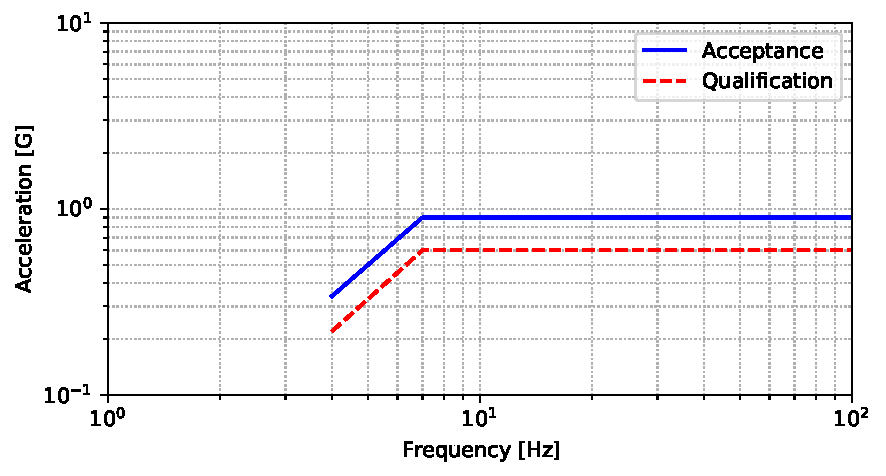
\includegraphics[width=\textwidth]{curves/sine_test.pdf}
        \caption{Sinusoidal sweeping vibration curve.}
        \label{fig:vibration-sinusoidal-curve}
    \end{center}
\end{figure}

\begin{figure}[!ht]
    \begin{center}
        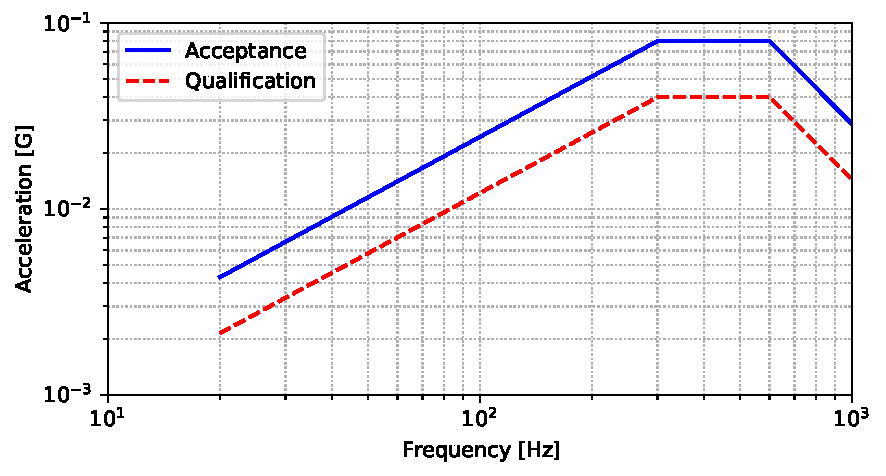
\includegraphics[width=\textwidth]{curves/random_vibration.pdf}
        \caption{Random vibration curve.}
        \label{fig:vibration-test}
    \end{center}
\end{figure}

\subsubsection{Thermal Test}

For the thermal tests, thermocouples should be attached on different points on the surface of the satellite, including over the solar panels and structure. As an example, \autoref{fsat-thermal-test} shows FloripaSat-I ready for thermal tests. The parameters of the tests are indicated in \autoref{tab:fsat-thermal-cycling}.

\begin{figure}[!ht]
    \begin{center}
        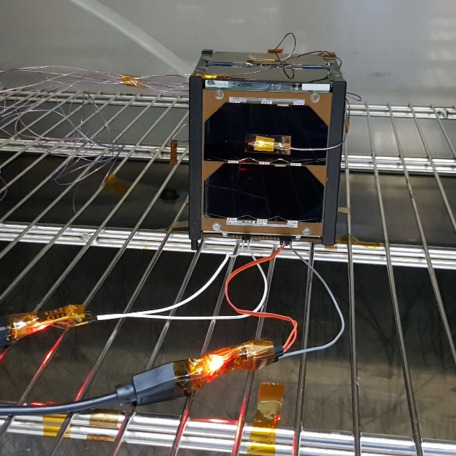
\includegraphics[width=0.5\textwidth]{figures/fsat_fm_thermal_cycling.jpg}
        \caption{FloripaSat-I during the thermal cycling (with thermocouples).}
        \label{fig:fsat-thermal-test}
    \end{center}
\end{figure}

\begin{table}[!h]
    \begin{center}
        \begin{tabular}{llll}
            \toprule[1.5pt]
            \multicolumn{2}{c}{\textbf{Thermal cycle}}  & \multicolumn{2}{c}{\textbf{Bake out}}        \\
            \midrule
            \textbf{Parameter}     & \textbf{Value}     & \textbf{Parameter} & \textbf{Value}          \\
            \midrule
            Number of cycles       & 2                  & \multicolumn{2}{c}{Part 1}                   \\
            \cmidrule{3-4}
            Min. temp. ($T_{min}$) & -15 $^\circ$C      & Pressure           & <1$\times 10^{-4}$ mbar \\
            Max. temp. ($T_{max}$) & +50 $^\circ$C      & Temperature        & 23 $^\circ$C            \\
            Duration in $T_{min}$  & 30 min             & Duration           & 12 hours                \\
            \cmidrule{3-4}
            Duration in $T_{max}$  & 60 min             & \multicolumn{2}{c}{Part 2}                   \\
            \cmidrule{3-4}
            Heating rate           & 5.5 $^\circ$C/min  & Pressure           & <1$\times 10^{-4}$ mbar \\
            Cooling rate           & 3.5 $^\circ$C/min  & Temperature        & 60 $^\circ$C            \\
            Stabilization criteria & 1 $^\circ$C/10 min & Duration           & 6 hours                 \\
            \bottomrule[1.5pt]
        \end{tabular}
        \caption{Parameters for the bake out and thermal cycling.}
        \label{tab:fsat-thermal-cycling}
    \end{center}
\end{table}



\section{Preliminary Results}


\subsubsection{Output Power of the Radio Modules}

The output power of the radio modules can be measured using a spectrum analyzer, as can be seen in the picture of \autoref{fig:rf-output-power-test}.

\begin{figure}[!ht]
    \begin{center}
        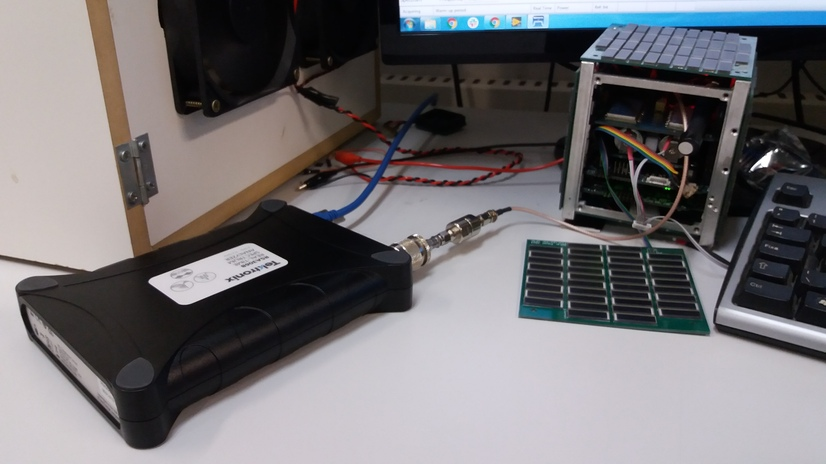
\includegraphics[width=\textwidth]{figures/rf-output-power-test.jpg}
        \caption{RF output power test with the radio modules connected to a spectrum analyzer.}
        \label{fig:rf-output-power-test}
    \end{center}
\end{figure}

The measured values for the beacon and downlink transmitters are available in Figures \ref{fig:beacon-power} and \ref{fig:downlink-power} respectively.

\begin{figure}[!ht]
    \begin{center}
        \includegraphics[width=\textwidth]{curves/beacon_output_power.pdf}
        \caption{Output power of the beacon radio.}
        \label{fig:beacon-power}
    \end{center}
\end{figure}

\begin{figure}[!ht]
    \begin{center}
        \includegraphics[width=\textwidth]{curves/downlink_output_power.pdf}
        \caption{Output power of the downlink radio.}
        \label{fig:downlink-power}
    \end{center}
\end{figure}

    %
% operation.tex
%
% Copyright (C) 2020 by SpaceLab.
%
% FloripaSat-2 Documentation
%
% This work is licensed under the Creative Commons Attribution-ShareAlike 4.0
% International License. To view a copy of this license,
% visit http://creativecommons.org/licenses/by-sa/4.0/.
%

%
% \brief Operation planning chapter.
%
% \author Gabriel Mariano Marcelino <gabriel.mm8@gmail.com>
%
% \institution Universidade Federal de Santa Catarina (UFSC)
%
% \version 0.1.0
%
% \date 2020/06/06
%

\chapter{Operation Planning} \label{ch:operation}

.

    %
% references.tex
%
% Copyright (C) 2021 by SpaceLab.
%
% GOLDS-UFSC Documentation
%
% This work is licensed under the Creative Commons Attribution-ShareAlike 4.0
% International License. To view a copy of this license,
% visit http://creativecommons.org/licenses/by-sa/4.0/.
%

%
% \brief References chapter.
%
% \author Gabriel Mariano Marcelino <gabriel.mm8@gmail.com>
%
% \institution Universidade Federal de Santa Catarina (UFSC)
%
% \version 0.1.0
%
% \date 2020/06/05
%

\bibliography{references/edc,%
              references/obdh2,%
              references/ttc,%
              references/eps2,%
              references/bat4c,%
              references/pc104-boards,%
              references/iip,%
              references/flatsat,%
              references/isis-antenna,%
              references/santoni2009,%
              references/gerhardt2010,%
              references/francois2010,%
              references/rigo2019,%
              references/ctj30,%
              references/icr18650-30b,%
              references/larson2005,%
              references/gpredict,%
              references/spacelab-decoder,%
              references/a719b,%
              references/2mcp14,%
              references/g5500,%
              references/ic9700,%
              references/b210,%
              references/cds,%
              references/floripasat}

\addcontentsline{toc}{chapter}{References}

    %
% appendices.tex
%
% Copyright The FloripaSat-2 Contributors.
%
% FloripaSat-2 Documentation
%
% This work is licensed under the Creative Commons Attribution-ShareAlike 4.0
% International License. To view a copy of this license,
% visit http://creativecommons.org/licenses/by-sa/4.0/.
%

%
% \brief Appendices.
%
% \author Gabriel Mariano Marcelino <gabriel.mm8@gmail.com>
%
% \version 0.2.0
%
% \date 2021/02/06
%

\begin{appendices}

%
% link_budget.tex
%
% Copyright (C) 2021 by SpaceLab.
%
% FloripaSat-2 Documentation
%
% This work is licensed under the Creative Commons Attribution-ShareAlike 4.0
% International License. To view a copy of this license,
% visit http://creativecommons.org/licenses/by-sa/4.0/.
%

%
% \brief Link budget calculation appendix.
%
% \author Gabriel Mariano Marcelino <gabriel.mm8@gmail.com>
%
% \institution Universidade Federal de Santa Catarina (UFSC)
%
% \version 0.2.0
%
% \date 2021/02/06
%

\chapter{Link Budget Calculation} \label{anx:link-budget}

This appendix shows the link budget calculation of all the satellite links (including the radio links of the payloads). The used method was taken from \cite{larson2005} (section 13.3).

\section{Distance to Satellite at Horizon}

The distance to satellite at horizon (the maximum theoretical distance between the satellite and a ground station) can be calculated using \autoref{eq:horizon-distance}.

\begin{equation} \label{eq:horizon-distance}
d = \sqrt{2\cdot R_{e}\cdot h + h^{2}}
\end{equation}

Where:

\begin{itemize}
    \item $R_{e}$ = Earth radius = 6378 km
    \item $h$ = Satellite altitude = 550 km
    \item $d$ = Distance to sattellite at horizon
\end{itemize}

So, the distance to satellite at horizon is:

\begin{equation} \label{eq:horizon-distance-result}
d = \sqrt{2\cdot 6378\cdot 550 + 550^{2}} = \mathbf{2705\ km}
\end{equation}

\section{Free-Space Path Loss}

The free-space path loss ($FSPL$) can be calculated using \autoref{eq:fspl}.

\begin{equation} \label{eq:fspl}
FSPL = \left( \frac{4\pi d f}{c} \right)^{2}
\end{equation}

Where:

\begin{itemize}
    \item $d$ = Distance between the satellite and the ground station
    \item $f$ = Radio frequency
    \item $c$ = Speed of light
\end{itemize}

The FSPL value in decibels can be calculated with \autoref{eq:fsbl-db}.

\begin{equation} \label{eq:fsbl-db}
    \begin{split}
        FSPL^{dB} & = 20\log\left(\frac{4\pi}{c}\right) + 20\log\left(d\right) + 20\log\left(f\right) \\
                  & = 32,45 + 20\log\left(\frac{d}{1\ km}\right) + 20\log\left(\frac{f}{1\ MHz}\right) \\
    \end{split}
\end{equation}

The minimum distance between the satellite and a ground station is the satellite altitude, in this case: 600 km. The maximum distance is the distance at horizon, defined by \autoref{eq:horizon-distance-result}.

\subsection{Beacon}

Considering the frequency of the beacon as 437 MHz, the minimum and maximum FSBL is:

\begin{equation}
    FSPL^{dB}_{min} = 32,45 + 20\log\left(\frac{550}{1\ km}\right) + 20\log\left(\frac{437}{1\ MHz}\right) = \mathbf{140,1\ dB}
\end{equation}

\begin{equation}
    FSPL^{dB}_{max} = 32,45 + 20\log\left(\frac{2705}{1\ km}\right) + 20\log\left(\frac{437}{1\ MHz}\right) = \mathbf{153,9\ dB}
\end{equation}

\begin{equation}
    \mathbf{140,1 \leq FSPL^{dB} \leq 153,9\ dB}
\end{equation}

\subsection{Downlink/Uplink}

Considering the frequency of the downlink/uplink as 462,5 MHz, the minimum and maximum FSBL is:

\begin{equation}
    FSPL^{dB}_{min} = 32,45 + 20\log\left(\frac{550}{1\ km}\right) + 20\log\left(\frac{462,5}{1\ MHz}\right) = \mathbf{140,6\ dB}
\end{equation}

\begin{equation}
    FSPL^{dB}_{max} = 32,45 + 20\log\left(\frac{2705}{1\ km}\right) + 20\log\left(\frac{462,5}{1\ MHz}\right) = \mathbf{154,4\ dB}
\end{equation}

\begin{equation}
    \mathbf{140,6 \leq FSPL^{dB} \leq 154,4\ dB}
\end{equation}

\subsection{Uplink (Payload)}

Considering the frequency of the payload's uplink is 401,635 MHz, the minimum and maximum FSBL is:

\begin{equation}
    FSPL^{dB}_{min} = 32,45 + 20\log\left(\frac{550}{1\ km}\right) + 20\log\left(\frac{401,635}{1\ MHz}\right) = \mathbf{139,3\ dB}
\end{equation}

\begin{equation}
    FSPL^{dB}_{max} = 32,45 + 20\log\left(\frac{2705}{1\ km}\right) + 20\log\left(\frac{401,635}{1\ MHz}\right) = \mathbf{153,2\ dB}
\end{equation}

\begin{equation}
    \mathbf{139,3 \leq FSPL^{dB} \leq 153,2\ dB}
\end{equation}

\section{Power at Receiver}

The power of the signal at the receiver can be estimated using \autoref{eq:power-at-receiver}.

\begin{equation} \label{eq:power-at-receiver}
    P_{r} = P_{t} + G_{t} + G_{r} - L_{p} - L_{s}
\end{equation}

Where:

\begin{itemize}
    \item $P_{r}$ = Power at the receiver
    \item $P_{t}$ = Transmitter power
    \item $G_{t}$ = Antenna gain of the transmitter
    \item $G_{r}$ = Antenna gain of the receiver
    \item $L_{p}$ = FSPL (Free-Space Path Loss)
    \item $L_{s}$ = Other losses in the system
\end{itemize}

Considering the worst scenario with the maximum possible distance between the satellite and a ground station, the power at the receiver for each link is calculated below.

\subsection{Beacon}

\begin{equation}
    P_{r} = 30 + 0 + 12 - 153,9 - 5 = -116,9\ dBm
\end{equation}

\begin{equation}
    \mathbf{P_{r} \geq -116,9\ dBm}
\end{equation}

\subsection{Downlink (UHF)}

\begin{equation}
    P_{r} = 30 + 0 + 12 - 154,4 - 5 = -117,4\ dBm
\end{equation}

\begin{equation}
    \mathbf{P_{r} \geq -117,4\ dBm}
\end{equation}

\subsection{Uplink (UHF)}

\begin{equation}
    P_{r} = 44 + 12 + 0 - 154,4 - 5 = -103,4\ dBm
\end{equation}

\begin{equation}
    \mathbf{P_{r} \geq -103,4\ dBm}
\end{equation}

\subsection{Uplink (Payload)}

\begin{equation}
    P_{r} = 30 + 3 + 0 - 153,2 - 5 = -125,2\ dBm
\end{equation}

\begin{equation}
    \mathbf{P_{r} \geq -125,2\ dBm}
\end{equation}

\section{Signal-to-Noise-Ratio}

The Signal-to-Noise-Ratio (SNR\nomenclature{\textbf{SNR}}{\textit{Signal To Noise Ratio}}) of a transmitted signal at the receiver can be expressed using \autoref{eq:snr}:

\begin{equation} \label{eq:snr}
    SNR = \frac{E_{b}}{N_{0}} = \frac{P_{t}G_{t}G_{r}}{kT_{s}RL_{p}}
\end{equation}

Where:

\begin{itemize}
    \item $P_{t}$ = Transmitter power
    \item $G_{t}$ = Antenna gain of the transmitter
    \item $G_{r}$ = Receiver gain
    \item $k$ = Boltzmann's constant ($\cong 1,3806 \times 10^{-23}\ J/K$)
    \item $T_{s}$ = System noise temperature
    \item $R$ = Data rate in bits per seconds (bps)
    \item $L_{p}$ = Free-Space Path Loss (FSPL)
\end{itemize}

The system noise temperature ($T_{s}$) can be defined using \autoref{eq:system-noise-temperature}.

\begin{equation} \label{eq:system-noise-temperature}
    T_{s} = T_{ant} + T_{r}
\end{equation}

with:

\begin{equation} \label{eq:noise-temperature-receiver}
    T_{r} = \frac{T_{0}}{L_{r}} (F - L_{r})
\end{equation}

and:

\begin{equation} \label{eq:noise-figure}
    F = 1 + \frac{T_{r}}{T_{0}}
\end{equation}

Combining Equations \ref{eq:system-noise-temperature}, \ref{eq:noise-temperature-receiver} and \ref{eq:noise-figure}:

\begin{equation} \label{eq:system-noise-temp-expanded}
    T_{s} = T_{ant} + \left( \frac{T_{0}(1 - L_{r})}{L_{r}} \right) + \left( \frac{T_{0} (F - 1)}{L_{r}} \right)
\end{equation}

Where:

\begin{itemize}
    \item $T_{ant}$ = Antenna noise temperature
    \item $T_{0}$ = Reference temperature (usually 290 K)
    \item $L_{r}$ = Line loss between the antenna and the receiver
    \item $F$ = Noise figure of the receiver
    \item $T_{r}$ = Noise temperature of the receiver
\end{itemize}

The SNR value in decibels can be calculated using the \autoref{eq:snr-db}:

\begin{equation} \label{eq:snr-db}
    \begin{split}
        SNR^{dB} & = 10\log_{10}\left( \frac{E_{b}}{N_{0}} \right) = 10\log_{10} \left( \frac{P_{t}G_{t}G_{r}}{kT_{s}RL_{p}} \right) \\
                 & = P_{t}^{dBm} - 30 + G_{t}^{dB} + G_{r}^{dB} - L_{p}^{dB} - 10\log k - 10\log T_{s} - 10\log R
    \end{split}
\end{equation}

Considering other losses in the system ($L_{s}$) (cable and connection losses as example), the \autoref{eq:snr-db} can be corrected as presented in \autoref{eq:snr-db-with-losses}.

\begin{equation} \label{eq:snr-db-with-losses}
    SNR^{dB} = P_{t}^{dBm} - 30 + G_{t}^{dB} + G_{r}^{dB} - L_{p}^{dB} - L_{s}^{dB} - 10\log k - 10\log T_{s} - 10\log R
\end{equation}

\subsection{Beacon}

Using Equations \ref{eq:snr-db-with-losses} and \ref{eq:system-noise-temperature}, with:

\begin{itemize}
    \item $P_{t} = 30\ dBm$
    \item $G_{t} = 0\ dBi$
    \item $G_{r} = 12\ dBi$
    \item $L_{p} = 153,9\ dB$
    \item $L_{s} = 5\ dB$
    \item $R = 4800\ bps$
    \item $T_{0} = 290\ K$
    \item $T_{r} = 290\ K$
    \item $T_{ant} = 300\ K$
    \item $F = 2\ dB$
    \item $L_{r} = 0,89\ (0,5\ dB)$
\end{itemize}

\begin{equation}
    T_{s} = 300 + \left( \frac{290 (1 - 0,89)}{0,89} \right) + \left( \frac{290 (2 - 1)}{0,89} \right) = 661,7\ K
\end{equation}

\begin{equation}
    SNR^{dB} = 30 - 30 + 0 + 12 - 153,9 - 5 + 228,6 - 28,21 - 36,81 = 16,68\ dB
\end{equation}

\begin{equation}
\mathbf{SNR^{dB} \geq 16,68\ dB}
\end{equation}

\subsection{Downlink}

Using Equations \ref{eq:snr-db-with-losses} and \ref{eq:system-noise-temperature}, with:

\begin{itemize}
    \item $P_{t} = 30\ dBm$
    \item $G_{t} = 0\ dBi$
    \item $G_{r} = 12\ dBi$
    \item $L_{p} = 154,4\ dB$
    \item $L_{s} = 5\ dB$
    \item $R = 9600\ bps$
    \item $T_{0} = 290\ K$
    \item $T_{r} = 290\ K$
    \item $T_{ant} = 300\ K$
    \item $F = 2\ dB$
    \item $L_{r} = 0,89\ (0,5\ dB)$
\end{itemize}

\begin{equation}
    SNR^{dB} = 30 - 30 + 0 + 12 - 154,4 - 5 + 228,6 - 28,21 - 39,82 = 13,17\ dB
\end{equation}

\begin{equation}
\mathbf{SNR^{dB} \geq 13,17\ dB}
\end{equation}

\subsection{Uplink}

Using Equations \ref{eq:snr-db-with-losses} and \ref{eq:system-noise-temperature}, with:

\begin{itemize}
    \item $P_{t} = 44\ dBm$
    \item $G_{t} = 12\ dBi$
    \item $G_{r} = 0\ dBi$
    \item $L_{p} = 154,4\ dB$
    \item $L_{s} = 5\ dB$
    \item $R = 9600\ bps$
    \item $T_{0} = 290\ K$
    \item $T_{r} = 290\ K$
    \item $T_{ant} = 300\ K$
    \item $F = 2\ dB$
    \item $L_{r} = 0,89\ (0,5\ dB)$
\end{itemize}

\begin{equation}
    SNR^{dB} = 44 - 30 + 12 + 0 - 154,4 - 5 + 228,6 - 28,21 - 39,82 = 27,17\ dB
\end{equation}

\begin{equation}
    \mathbf{SNR^{dB} \geq 27,17\ dB}
\end{equation}

\subsection{Uplink (Payload)}

Using Equations \ref{eq:snr-db-with-losses} and \ref{eq:system-noise-temperature}, with:

\begin{itemize}
    \item $P_{t} = 30\ dBm$
    \item $G_{t} = 3\ dBi$
    \item $G_{r} = 0\ dBi$
    \item $L_{p} = 153,2\ dB$
    \item $L_{s} = 5\ dB$
    \item $R = 400\ bps$
    \item $T_{0} = 290\ K$
    \item $T_{r} = 290\ K$
    \item $T_{ant} = 300\ K$
    \item $F = 2\ dB$
    \item $L_{r} = 0,89\ (0,5\ dB)$
\end{itemize}

\begin{equation}
    SNR^{dB} = 30 - 30 + 3 + 0 - 153,2 - 5 + 228,6 - 28,21 - 26,02 = 19,17\ dB
\end{equation}

\begin{equation}
    \mathbf{SNR^{dB} \geq 19,17\ dB}
\end{equation}

\section{Link Margin}

From \cite{larson2005}, the minimum SNR value at the received considering a $10^{-5}$ bit error rate is:

\begin{itemize}
    \item Beacon: $SNR^{dB} \geq 9,6\ dB$
    \item Downlink/Uplink: $SNR^{dB} \geq 9,6\ dB$
    \item Uplink (payload): $SNR^{dB} \geq 9,6\ dB$
\end{itemize}

And considering the link margin as the SNR of the link minus the SNR threshold for a given bit error, the link margin of the radio links of the satellite are:

\begin{itemize}
    \item Beacon: $16,68 - 9,6 = \mathbf{7,077\ dB}$
    \item Downlink: $13,17 - 9,6 = \mathbf{3,574\ dB}$
    \item Uplink: $27,17 - 9,6 = \mathbf{17,57\ dB}$
    \item Uplink (payload): $19,17 - 9,6 = \mathbf{9,57\ dB}$
\end{itemize}

%
% packets.tex
%
% Copyright (C) 2021 by SpaceLab.
%
% FloripaSat-2 Documentation
%
% This work is licensed under the Creative Commons Attribution-ShareAlike 4.0
% International License. To view a copy of this license,
% visit http://creativecommons.org/licenses/by-sa/4.0/.
%

%
% \brief Telecommunication packets appendix.
%
% \author Gabriel Mariano Marcelino <gabriel.mm8@gmail.com>
%
% \institution Universidade Federal de Santa Catarina (UFSC)
%
% \version 0.9.0
%
% \date 2021/06/03
%

\chapter{Telecommunication Packets} \label{anx:packets}

This appendix lists all the packets used by the RF links of the satellite: Beacon, downlink and uplink. The fields and length of each type of packet is also presented.

\section{Beacon}

The \autoref{tab:beacon-packets} presents the content of the beacon packets.

\begin{longtable}[c]{lcL{0.4\textwidth}c}
    \toprule[1.5pt]
    \textbf{Packet} & \textbf{Position} & \textbf{Content} & \textbf{Length [bytes]} \\
    \midrule
    \multirow{22}{*}{EPS data} & 0  & Packet ID (00h)                       & 1 \\
                               & 1  & Source callsign (`` PY0EFS'')         & 7 \\
                               & 8  & Timestamp in ms                       & 4 \\
                               & 12 & Battery cell 1 voltage in mV          & 2 \\
                               & 14 & Battery cell 2 voltage in mV          & 2 \\
                               & 16 & Battery current in mA                 & 2 \\
                               & 18 & Battery charge in mAh                 & 2 \\
                               & 20 & Battery cell 1 temperature in K       & 2 \\
                               & 22 & Battery cell 2 temperature in K       & 2 \\
                               & 24 & Battery monitor temperature in K      & 2 \\
                               & 26 & Solar panel voltage in mV (-Y and +X) & 2 \\
                               & 28 & Solar panel voltage in mV (-X and +Z) & 2 \\
                               & 30 & Solar panel voltage in mV (-Z and +Y) & 2 \\
                               & 32 & Solar panel current in mA (-Y)        & 2 \\
                               & 34 & Solar panel current in mA (+Y)        & 2 \\
                               & 36 & Solar panel current in mA (-X)        & 2 \\
                               & 38 & Solar panel current in mA (+X)        & 2 \\
                               & 40 & Solar panel current in mA (-Z)        & 2 \\
                               & 42 & Solar panel current in mA (+Z)        & 2 \\
                               & 44 & Temperature of the EPS $\mu$C in K    & 2 \\
    \cmidrule{4-4}
                               &    &                                       & 46 \\
    \midrule
    \multirow{9}{*}{TTC data}  & 0  & Packet ID (01h)                       & 1 \\
                               & 1  & Source callsign (`` PY0EFS'')         & 7 \\
                               & 8  & Timestamp in ms                       & 4 \\
                               & 12 & Temperature of the TTC $\mu$C in K    & 2 \\
                               & 14 & Reset counter                         & 2 \\
                               & 16 & Last reset cause                      & 1 \\
                               & 15 & Temperature of the beacon radio in K  & 2 \\
    \cmidrule{4-4}
                               &    &                                       & 19 \\
    \bottomrule[1.5pt]
    \caption{Beacon packets.}
    \label{tab:beacon-packets}
\end{longtable}

\section{Downlink}

In \autoref{tab:downlink-packets} the content of the downlink packets is available.

\begin{longtable}[c]{lcL{0.4\textwidth}c}
    \toprule[1.5pt]
    \textbf{Packet} & \textbf{Position} & \textbf{Content} & \textbf{Length [bytes]} \\
    \midrule
    \multirow{42}{*}{General telemetry}     & 0  & Packet ID (20h)                              & 1 \\
                                            & 1  & Source callsign (`` PY0EFS'')                & 7 \\
                                            & 8  & Time counter in milliseconds                 & 4 \\
                                            & 12 & Temperature of the OBDH $\mu$C in Kelvin     & 2 \\
                                            & 14 & Input current of the OBDH in mA              & 2 \\
                                            & 16 & Input voltage of the OBDH in mV              & 2 \\
                                            & 18 & Last reset cause of the OBDH                 & 1 \\
                                            & 19 & Reset counter of the OBDH                    & 2 \\
                                            & 21 & Last valid telecommand (uplink packet ID)    & 1 \\
                                            & 22 & Temperature of the radio in Kelvin           & 2 \\
                                            & 24 & RSSI of the last valid telecommand           & 2 \\
                                            & 26 & Temperature of the antenna in Kelvin         & 2 \\
                                            & 28 & Antenna status                               & 2 \\
                                            & 30 & Payloads status                              & 1 \\
                                            & 31 & Temperature of the EPS $\mu$C in K           & 2 \\
                                            & 33 & EPS circuitry and Beacon MCU current in mA   & 2 \\
                                            & 35 & Last reset cause of the EPS                  & 1 \\
                                            & 36 & Reset counter (EPS)                          & 2 \\
                                            & 38 & -Y and +X sides solar panel voltage in mV    & 2 \\
                                            & 40 & -X and +Z sides solar panel voltage in mV    & 2 \\
                                            & 42 & -Z and +Y sides solar panel voltage in mV    & 2 \\
                                            & 44 & -Y side solar panel current in mA            & 2 \\
                                            & 46 & +Y side solar panel current in mA            & 2 \\
                                            & 48 & -X side solar panel current in mA            & 2 \\
                                            & 50 & +X side solar panel current in mA            & 2 \\
                                            & 52 & -Z side solar panel current in mA            & 2 \\
                                            & 54 & +Z side solar panel current in mA            & 2 \\
                                            & 55 & MPPT 1 duty cycle in \%                      & 1 \\
                                            & 56 & MPPT 2 duty cycle in \%                      & 1 \\
                                            & 57 & MPPT 3 duty cycle in \%                      & 1 \\
                                            & 59 & Main power bus voltage in mV                 & 2 \\
                                            & 61 & Batteries voltage in mV                      & 2 \\
                                            & 63 & Batteries current in mA                      & 2 \\
                                            & 65 & Batteries average current in mA              & 2 \\
                                            & 67 & Batteries accumulated current in mA          & 2 \\
                                            & 69 & Batteries charge in mAh                      & 2 \\
                                            & 71 & Battery monitor IC temperature in K          & 2 \\
                                            & 73 & Battery heater 1 duty cycle in \%            & 1 \\
                                            & 74 & Battery heater 2 duty cycle in \%            & 1 \\
                                            & 75 & Payload EDC status (00h=none, 01h=EDC\_1, 02h=EDC\_2, 03h=Both) & 1 \\
                                            & 76 & Payload-X status (00h=OFF,01h=ON)            & 1 \\
                                            & 77 & Radiation monitor status (00h=OFF,01h=ON)    & 1 \\
    \cmidrule{4-4}
                                            &    &                                              & 78 \\
    \multirow{3}{*}{Ping answer}            & 0  & Packet ID (21h)                      & 1 \\
                                            & 1  & Source callsign (`` PY0EFS'')        & 7 \\
                                            & 8  & Requester callsign                   & 7 \\
    \cmidrule{4-4}
                                            &    &                                      & 15 \\
    \multirow{6}{*}{Data request answer}    & 0  & Packet ID (22h)                      & 1 \\
                                            & 1  & Source callsign (`` PY0EFS'')        & 7 \\
                                            & 8  & Requester callsign                   & 7 \\
                                            & 15 & Data type ID                         & 1 \\
                                            & 16 & Timestamp                            & 4 \\
                                            & 20 & Data                                 & Var. \\
    \cmidrule{4-4}
                                            &    &                                      & 20 (min.) \\
    \multirow{5}{*}{Message broadcast}      & 0  & Packet ID (23h)                      & 1 \\
                                            & 1  & Source callsign (`` PY0EFS'')        & 7 \\
                                            & 8  & Requester callsign                   & 7 \\
                                            & 15 & Destination callsign                 & 7 \\
                                            & 22 & Message                              & up to 38 \\
    \cmidrule{4-4}
                                            &    &                                      & 22 to 60 \\
                                            & 0  & Packet ID (24h)                      & 1 \\
                                            & 1  & Source callsign (`` PY0EFS'')        & 7 \\
                                            & 8  & Payload ID (01h or 02h)              & 1 \\
                                            & 9  & PTT signal receiving time            & 4 \\
                                            & 13 & Error code                           & 1 \\
                                            & 14 & Carrier frequency                    & 2 \\
                                            & 16 & Carrier amplitude at ADC interface output & 2 \\
                                            & 18 & User message length in bytes         & 1 \\
                                            & 19 & ARGOS-2 PTT-A2 user message          & 35 \\
                                            & 54 & Current time since J2000 epoch       & 4 \\
                                            & 58 & Elapsed time since last reset        & 4 \\
   Payload data                             & 62 & System current supply in mA          & 2 \\
   (EDC info)                               & 64 & System voltage supply in mV          & 2 \\
                                            & 65 & EDC board temperature                & 1 \\
                                            & 66 & RF front end LO                      & 1 \\
                                            & 67 & RMS level at front-end output        & 2 \\
                                            & 69 & Generated PTT packages since last initialization & 1 \\
                                            & 70 & Max                                  & 1 \\
                                            & 71 & Memory error count                   & 1 \\
                                            & 72 & Current time                         & 4 \\
                                            & 76 & Number of PTT package available for reading & 1 \\
                                            & 77 & PTT decoder task status              & 1 \\
                                            & 78 & ADC sampler state                    & 1 \\
    \cmidrule{4-4}
                                            &    &                                      & 79 \\
                                            & 0  & Packet ID (24h)                      & 1 \\
                                            & 1  & Source callsign (`` PY0EFS'')        & 7 \\
                                            & 8  & Payload ID (01h or 02h)              & 1 \\
                                            & 9  & Elapsed time since J2000 epoch       & 4 \\
    Payload data                            & 13 & ADC sample packet number             & 1 \\
    (EDC samples)                           & 14 & First ADC I-sample                   & 2 \\
                                            & 16 & First ADC Q-sample                   & 2 \\
                                            & ... & ...                                 & ... \\
                                            & 214 & N ADC I-sample                      & 2 \\
                                            & 216 & N ADC Q-sample                      & 2 \\
    \cmidrule{4-4}
                                            &    &                                      & 218 \\
    \multirow{5}{*}{TC feedback}            & 0  & Packet ID (25h)                      & 1 \\
                                            & 1  & Source callsign (`` PY0EFS'')        & 7 \\
                                            & 8  & Requester callsign                   & 7 \\
                                            & 15 & TC packet ID                         & 1 \\
                                            & 16 & Timestamp                            & 4 \\
    \cmidrule{4-4}
                                            &    &                                      & 20 \\
    \bottomrule[1.5pt]
    \caption{Downlink packets.}
    \label{tab:downlink-packets}
\end{longtable}

\section{Uplink}

The \autoref{tab:uplink-packets} presents the content of the uplink packets.

\begin{longtable}[c]{lcL{0.4\textwidth}c}
    \toprule[1.5pt]
    \textbf{Packet} & \textbf{Position} & \textbf{Content} & \textbf{Length [bytes]} \\
    \midrule
    \multirow{2}{*}{Ping request}       & 0  & Packet ID (40h)                      & 1 \\
                                        & 1  & Ground station callsign              & 7 \\
    \cmidrule{4-4}
                                        &    &                                      & 8 \\
    \multirow{6}{*}{Data request}       & 0  & Packet ID (41h)                      & 1 \\
                                        & 1  & Ground station callsign              & 7 \\
                                        & 8  & Data type ID                         & 1 \\
                                        & 9  & Start timestamp                      & 4 \\
                                        & 13 & End timestamp                        & 4 \\
                                        & 17 & HMAC hash                            & 20 \\
    \cmidrule{4-4}
                                        &    &                                      & 37 \\
    \multirow{4}{*}{Broadcast message}  & 0  & Packet ID (42h)                      & 1 \\
                                        & 1  & Ground station callsign              & 7 \\
                                        & 8  & Destination callsign                 & 7 \\
                                        & 15 & Message                              & up to 38 \\
    \cmidrule{4-4}
                                        &    &                                      & up to 53 \\
    \multirow{4}{*}{Enter hibernation}  & 0  & Packet ID (43h)                      & 1 \\
                                        & 1  & Ground station callsign              & 7 \\
                                        & 8  & Hibernation in hours                 & 2 \\
                                        & 10 & HMAC hash                            & 20 \\
    \cmidrule{4-4}
                                        &    &                                      & 30 \\
    \multirow{3}{*}{Leave hibernation}  & 0  & Packet ID (44h)                      & 1 \\
                                        & 1  & Ground station callsign              & 7 \\
                                        & 8  & HMAC hash                            & 20 \\
    \cmidrule{4-4}
                                        &    &                                      & 28 \\
    \multirow{4}{*}{Activate module}    & 0  & Packet ID (45h)                      & 1 \\
                                        & 1  & Ground station callsign              & 7 \\
                                        & 8  & Module ID                            & 1 \\
                                        & 9  & HMAC hash                            & 20 \\
    \cmidrule{4-4}
                                        &    &                                      & 29 \\
    \multirow{4}{*}{Deactivate module}  & 0  & Packet ID (46h)                      & 1 \\
                                        & 1  & Ground station callsign              & 7 \\
                                        & 8  & Module ID                            & 1 \\
                                        & 9  & HMAC hash                            & 20 \\
    \cmidrule{4-4}
                                        &    &                                      & 29 \\
    \multirow{4}{*}{Activate payload}   & 0  & Packet ID (47h)                      & 1 \\
                                        & 1  & Ground station callsign              & 7 \\
                                        & 8  & Payload ID                           & 1 \\
                                        & 9  & HMAC hash                            & 20 \\
    \cmidrule{4-4}
                                        &    &                                      & 29 \\
    \multirow{4}{*}{Deactivate payload} & 0  & Packet ID (48h)                      & 1 \\
                                        & 1  & Ground station callsign              & 7 \\
                                        & 8  & Payload ID                           & 1 \\
                                        & 9  & HMAC hash                            & 20 \\
    \cmidrule{4-4}
                                        &    &                                      & 29 \\
    \multirow{3}{*}{Erase memory}       & 0  & Packet ID (49h)                      & 1 \\
                                        & 1  & Ground station callsign              & 7 \\
                                        & 8  & HMAC hash                            & 20 \\
    \cmidrule{4-4}
                                        &    &                                      & 28 \\
    \multirow{3}{*}{Force reset}        & 0  & Packet ID (4Ah)                      & 1 \\
                                        & 1  & Ground station callsign              & 7 \\
                                        & 8  & HMAC hash                            & 20 \\
    \cmidrule{4-4}
                                        &    &                                      & 28 \\
    \multirow{5}{*}{Get payload data}   & 0  & Packet ID (4Bh)                      & 1 \\
                                        & 1  & Ground station callsign              & 7 \\
                                        & 8  & Payload ID                           & 1 \\
                                        & 9  & Payload arguments                    & 12 \\
                                        & 21 & HMAC hash                            & 20 \\
    \cmidrule{4-4}
                                        &    &                                      & 41 \\
    \bottomrule[1.5pt]
    \caption{Uplink packets.}
    \label{tab:uplink-packets}
\end{longtable}

%
% packets.tex
%
% Copyright The FloripaSat-2 Contributors.
%
% FloripaSat-2 Documentation
%
% This work is licensed under the Creative Commons Attribution-ShareAlike 4.0
% International License. To view a copy of this license,
% visit http://creativecommons.org/licenses/by-sa/4.0/.
%

%
% \brief EDC test report appendix.
%
% \author Gabriel Mariano Marcelino <gabriel.mm8@gmail.com>
%
% \version 0.9.0
%
% \date 2022/03/12
%

\chapter{EDC Test Report} \label{anx:edc-report}

\begin{figure}[!htb]
    \begin{center}
        \subfigure[Top side.\label{fig:edc-top-test}]{\includegraphics[width=\textwidth]{figures/edc_report/edcs-top}}

        \subfigure[Bottom side.\label{fig:edc-bottom-test}]{\includegraphics[width=\textwidth]{figures/edc_report/edcs-bottom}}
        \caption{Tested EDC boards.}
        \label{fig:edc-boards-test}
    \end{center}
\end{figure}

\section{Command interface test}

\subsection{Used material}

\begin{itemize}
    \item EDC boards
    \item USB-UART coverter
    \item Saleae Logic Analyzer
    \item Protoboard
    \item Desktop computer
    \item Logic 2 software
    \item Cutecom software
    \item USB cables
    \item Pin header wires
\end{itemize}

\begin{figure}[!ht]
    \begin{center}
        \includegraphics[width=\textwidth]{figures/edc_report/cmd-test-setup}
        \caption{Setup of the EDC's command interface test.}
        \label{fig:edc-test-setup}
    \end{center}
\end{figure}

\subsection{Results}

\begin{figure}[!ht]
    \begin{center}
        \includegraphics[width=\textwidth]{figures/edc_report/edc-cmd-issue}
        \caption{Command interface issue.}
        \label{fig:edc-cmd-issue}
    \end{center}
\end{figure}

\begin{figure}[!ht]
    \begin{center}
        \includegraphics[width=0.6\textwidth]{figures/edc_report/edc-bd-uart-if}
        \caption{UART and RS-485 interfaces of the EDC.}
        \label{fig:edc-bd-uart-if}
    \end{center}
\end{figure}

\begin{figure}[!ht]
    \begin{center}
        \includegraphics[width=\textwidth]{figures/edc_report/echo-cmd}
        \caption{``Echo'' command demonstration.}
        \label{fig:edc-echo-cmd}
    \end{center}
\end{figure}

\section{RF chain test}

\subsection{Used material}

\begin{itemize}
    \item EDC boards
    \item USB-UART converter
    \item Ettus USRP B210 SDR
    \item Desktop computer
    \item GNURadio v3.9
    \item Cutecom software
    \item USB cables
    \item Pin header wires
    \item SMA coaxial cable
    \item 30 dB attenuator
\end{itemize}

\begin{figure}[!ht]
    \begin{center}
        \includegraphics[width=\textwidth]{figures/edc_report/rf-chain-setup}
        \caption{Setup of the EDC's RF chain test.}
        \label{fig:edc-rf-chain-test-setup}
    \end{center}
\end{figure}

\begin{figure}[!ht]
    \begin{center}
        \includegraphics[width=\textwidth]{figures/edc_report/edc-rf-test-signal}
        \caption{Generated signal used in the RF chain test.}
        \label{fig:edc-rf-signal}
    \end{center}
\end{figure}

\subsection{Results}

.


\end{appendices}


\end{document}
